% !TEX TS-program = pdflatex
% !TEX encoding = UTF-8 Unicode
\RequirePackage{fix-cm}
\documentclass[ngerman,a4paper,openany,showtrims]{memoir}
%!TEX ROOT = ersti.tex

\usepackage[ngerman]{babel}
\usepackage{color}

\usepackage[utf8]{inputenc} % wir wollen das erstiinfo /richtig/
                            % kodiert haben

% Boolean, mit dem wir abfragen können, ob Druck- oder Webversion benötigt wird,
% um nicht alles in config_druck.tex bzw. config_web.tex angeben zu müssen.
\usepackage{ifthen}
\newboolean{druckversion}

% Diese Datei wird automatisch vom Makefile erstellt aus config_web.tex
% und config_druck.tex, je nachdem was man will
\input{config.tex}

\usepackage{eurosym} % eurozeichen kann man schon gut gebrauchen
\usepackage{amsmath}

\usepackage{memhfixc} % fix für die kollision memoir/hyperref

\usepackage{euler} % euler ist die schrift für die kapitelüberschriften
\usepackage{wasysym}  % für die Simleys
\usepackage[squaren]{SIunits}  % für "m^2" und andere Maßeinheiten
\usepackage{newcent}
\usepackage[pdftex]{graphicx} % hübsche bilder
\usepackage{epstopdf} % direkt eps einbinden können
\usepackage{booktabs} % hübsche tabellen
\usepackage[protrusion=true,expansion]{microtype} % hübscherer Blocksatz
\usepackage{multirow} % mehrzeilige Spalten in Tabellen
\usepackage[T1]{fontenc}
\usepackage{subcaption} %für subfigures
\usepackage{enumitem} % für descriptions mit style=unboxed
\usepackage{dblfloatfix}    % To enable figures at the bottom of page

\usepackage[section=chapter,numberedsection=false,numberline,nonumberlist]{glossaries}
\renewcommand*{\glsclearpage}{\clearpage}
\makeglossaries
% Kurzanleitung:
% http://mirror.ctan.org/macros/latex/contrib/glossaries/glossariesbegin.pdf

% Syntax:
% \newglossaryentry{ label }{ settings }
% \newacronym{ label }{ abbrv }{ full }


% Beispiele: Einträge erstellen
% \newglossaryentry{electrolyte}{name=electrolyte, description={solution able to conduct electric current}}

% \newglossaryentry{oesophagus}{name=œsophagus, description={canal from mouth to stomach}, plural=œsophagi}

% \newacronym{label}{svm}{support vector machine}


% Beispiel: sich auf einen Glossareintrag beziehen
%       \gls{ label }
%       \glspl{ label }   % gibt die Pluralform aus


\newglossaryentry{c.t.}{name={c.t.}, description={lat.: cum tempore, mit Zeit, also eine viertel Stunde später}}
\newglossaryentry{s.t.}{name={s.t.}, description={lat.: sine tempore, ohne Zeit, also genau so, wie es da steht}}
\newglossaryentry{HEIDI}{name={HEIDI}, description={So heißt das Computersystem der \gls{UB}, mit dem ihr nach Büchern suchen und sie auch gleich vorbestellen könnt. Eure aktuellen Ausleihen werden auch dort gelistet, ebenso besteht die Möglichkeit dort insgesamt zweimal eure Ausleihfristen um je einen Monat zu verlängern. Die Adresse ist \url{heidi.ub.uni-heidelberg.de}, aber eine Suche nach \emph{heidi heidelberg} führt auch zum Ziel}}


\newglossaryentry{URZ}{
	name={URZ},
	first={Universitätsrechenzentrum (URZ)},
	description={Das Universitätsrechenzentrum stellt alles bereit, was sich grob mit dem Begriff \emph{Computer} in Verbindung bringen lässt. Siehe Artikel auf \autopageref{urz}}
}

\newglossaryentry{AM}{
	name={AM},
	first={Angewandte Mathematik},
	description={Die Angewandte Mathematik ist eines der Institute der Fakultät für Mathematik und Informatik und sitzt im Mathematikon}
}

\newglossaryentry{IAM}{
	name={IAM},
	first={Institut für Angewandte Mathematik},
	description={siehe \Gls{AM}}
}

\newglossaryentry{MI}{
	name={MI},
	first={Mathematisches Institut},
	description={Das Mathematisches Institut -- auch Reine Mathematik genannt -- ist eines der Institute der Fakultät für Mathematik und Informatik und sitzt im Mathematikon im 3. OG}
}

\newglossaryentry{RM}{
	name={RM},
	first={Reine Mathematik},
	description={siehe \Gls{MI}}
}

\newglossaryentry{IfI}{
	name={IfI},
	first={Institut für Informatik},
	description={Das Institut für Informatik ist eines der Institute der Fakultät für Mathematik und Informatik und sitzt im Mathematikon. Die Mitglieder decken unter anderem einen Großteil der Lehre im Bereich Informatik ab}
}

\newglossaryentry{Mathematikon}{
    name={Mathematikon},
	first={Mathematikon},
	description={Das Mathematikon (INF 205) ist das neu gebaute Ge\-bäu\-de an der Berliner Straße, in dem die Fakultät für Mathematik und Informatik und das IWR untergebracht sind. Dort finden auch die meisten Seminare, Übungen und kleinere Vorlesungen statt. Außerdem befindet sich dort die Bereichsbibliothek, einige Arbeitsplätze und natürlich die Fachschaft}
}

\newglossaryentry{FSK}{
	name={FSK},
	first={Fachschaftskonferenz (FSK)},
	description={Die Fachschaftskonferenz war die Vorgängerin des StuRa als Vertretung aller Studis vor der Wiedereinführung der Verfassten Studierendenschaft}
}

\newglossaryentry{StuRa}{
	name={StuRa},
	first={Studierendenrat (StuRa)},
	description={Der StuRa ist das Zentralorgan der Verfassten Studierendenschaft an der Uni Heidelberg und tagt zweiwöchentlich im neuen Hörsaal am Philosophenweg. Details in den Artikeln auf \autopageref{hopo} ff}
}

\newglossaryentry{ZFB}{
	name={ZFB},
	first={Zentrales Fachschaftenbüro (ZFB)},
	description={siehe \Gls{StuRa-Buero}}
}

\newglossaryentry{StuRa-Buero}{
	name={StuRa-Büro},
	first={StuRa-Büro},
	description={früher auch: \Gls{ZFB}. Büro- und Tagungsräume für den StuRa und andere studentische Gruppen. Auch die Sozialberatung u.ä. finden hier statt. Die genaue Adresse ist Albert-Ueberle-Straße 3-5, 69120 Heidelberg}
}


\newacronym{UB}{UB}{Universitätsbibliothek}
\newacronym{OPNV}{ÖPNV}{Öffentlicher Personen Nahverkehr}
\newacronym{INF}{INF}{im Neuenheimer Feld}
\newacronym{HS}{HS}{Hörsaal}
\newglossaryentry{FSWE}{
	name={FSWE},
	first={Fachschaftswochenende (FSWE)},
	description={Das Fachschaftswochenende veranstalten wir einmal pro Semester, um Themen diskutieren zu können, die sich nicht sinnvoll in einer Fachschaftssitzung unterbringen lassen. Und natürlich um jede Menge Spaß zu haben \smiley. Die Mitfahrt ist für euch kostenlos}
}

\newglossaryentry{SWS}{
	name={SWS},
	first={Semesterwochenstunden (SWS)},
	description={Die Semesterwochenstunden geben an, wie viel Aufwand eine Veranstaltung ungefähr ist. Genau genommen wird nur die Anwesenheitszeit pro Woche angegeben: Ein Seminar hat dann meist 2 SWS, eine Vorlesung mit Übung dagegen 4+2 SWS}
}

\newglossaryentry{LP}{
	name={LP},
	first={Leistungspunkte (LP)},
	description={Leistungspunkte -- auch Credit Points (CP) oder ECTS (European Transfer Credit System) genannt -- sind ein Maß für den Aufwand eines Moduls. Dabei sollte ein LP etwa 30 Stunden Arbeit entsprechen -- das kommt aber öfter nicht als hin}
}

\newglossaryentry{CP}{
	name={CP},
	first={Credit Points (CP)},
	description={siehe \Gls{LP}}
}
\newglossaryentry{ECTS}{
	name={ECTS},
	first={European Credit Transfer System},
	description={Die Erfindung, die uns Leistungspunkte beschert hat; Wird häufig auch dafür verwendet, siehe \Gls{LP}}
}


\newacronym{ZUV}{ZUV}{Zentrale Universitätsverwaltung}
\newacronym{StuWe}{StuWe}{\href{www.studentenwerk.uni-heidelberg.de}{Studierendenwerk}}

% Für bestimmte Akronyme, die keine Mehrzahl haben, missbrauchen wir das
% Mehrzahlfeld um Genitiv (oder so… "des KIPs") zu speichern
\newacronym[\glslongpluralkey={Kirchhoff-Instituts für Physik},\glsshortpluralkey={KIP}]{KIP}{KIP}{Kirchhoff-Institut für Physik}
\newglossaryentry{PI}{
	name={PI},
	first={Phy\-si\-ka\-li\-sches Institut (PI)},
	description={Das Physikalische Institut wird des Öfteren auch Klaus-Tschira-Gebäude genannt. Es handelt sich dabei um eines der neueren Gebäude im Feld. Dort finden eure ersten verpflichtenden Physikpraktika statt, welche aus diversen Versuchen bestehen}
}
\newglossaryentry{ITP}{
	name={ITP},
	first={Institut für Theoretische Physik (ITP)},
	description={Das Institut für Theoretische Physik bevölkert die meisten Uni-Ge\-bäu\-de am Philosophenweg. Ihr findet die Dozentinnen und Mitarbeiterinnen in den Gebäuden Philosophenweg 12, 16 und 19. Außerdem gibt es insbesondere in der 12 noch einige Seminarräume}
}
\newacronym[\glslongpluralkey={Verkehrsverbundes Rhein-Neckar},\glsshortpluralkey={VRN}]{VRN}{VRN}{Verkehrsverbund Rhein-Neckar}

%Vorlesungstitel und deren Abkürzungen:
%Informatik
\newglossaryentry{IPI}{name=IPI, description={Die Vorlesung Einführung in die Praktische Informatik, wird manchmal auch Info1 genannt}}
\newglossaryentry{ITI}{name=ITI, description={Die Vorlesung Einführung in die Technische Informatik, kurz auch einfach Technische Info}}
\newglossaryentry{IDB1}{name=IDB1, description={Die Vorlesung Datenbanken 1}}
\newglossaryentry{BeNe}{name=BeNe, description={Die Vorlesung Betriebssysteme und Netzwerke, im  Modulhandbuch mit IBN abgekürzt}}
\newglossaryentry{ISW}{name=ISW, description={Die Vorlesung Einführung in Software Engineering}}
\newglossaryentry{IPK}{name=IPK, description={Programmierkurs}}
\newglossaryentry{MafIn}{name=MafIn, description={Die Vorlesungen Mathematik für Informatiker 1 und 2, im  Modulhandbuch mit IMI abgekürzt}}
\newglossaryentry{AlDa}{name=AlDa, description={Die Vorlesung Algorithmen und Datenstrukturen, im Modulhandbuch mit IAD abgekürzt}}
%Mathe
\newglossaryentry{LA}{name=LA, description={Die Vorlesungen Lineare Algebra 1 und 2, selten auch LinA genannt}}
\newglossaryentry{Ana}{name=Ana, description={Die Vorlesungen Analysis 1 und 2 sowie Höhere Analysis -- letztere wird manchmal auch Analysis 3 genannt}}
\newglossaryentry{Num0}{name=Num0, description={Die Vorlesung Einführung in die Numerik}}
\newglossaryentry{WTheo0}{name=WTheo0, description={Die Vorlesung Einführung in die Wahrscheinlichkeitstheorie und Statistik}}
\newglossaryentry{FunkTheo}{name=Funktheo, description={Die Vorlesungen Funktionentheorie 1 und 2}}
%Physik
\newglossaryentry{Ex}{name=Ex, description={Die Vorlesungen Experimentalphysik 1 bis~5}}
\newglossaryentry{HoMa}{name=HöMa, description={Die Vorlesungen Höhere Mathematik für Physiker 2 und 3 (HöMa 1 gibt es nicht)}}
%Physik&Info
\newglossaryentry{Theo}{name=Theo, description={Physik: Die Vorlesungen Theoretische Physik 1 bis 4. Informatik: Die Vorlesung Einführung in die Theoretische Informatik, im Modulhandbuch mit ITH abgekürzt}}
\newglossaryentry{AP}{name=AP, description={Physik: Das Physikalische Praktikum für Anfänger 1 und 2, meist Anfängerpraktikum genannt oder wie im Modulhandbuch mit PAP1 bzw. PAP2 abgekürzt. Informatik: Das (Software)-Anfängerpraktikum}}
\newglossaryentry{FP}{name=FP, description={Physik: Das Physikalische Fortgeschrittenenpraktikum 1 und 2, meist Fortgeschrittenenpraktikum genannt. Informatik: Das (Software)-Fortgeschrittenenpraktikum}}

% Zeige alle Einträge an, auch die ohne Referenz
\glsaddall


% alternative Fußnoten-Symbole
\makeatletter
\newcommand*{\@greek}[1]{\ensuremath{\ifcase#1 \or \alpha \or \beta \or \gamma \or \delta \or \varepsilon \or \zeta \or \eta \or \vartheta \or \iota \or \kappa \or \lambda \or \mu \or \nu \or o \or \pi \or \varrho \or \sigma \or \tau \or \upsilon \or \varphi \or \chi \or \psi \or \omega \or \varsigma \else \@cterr \fi}}
\newcommand*{\greek}[1]{\expandafter\@greek\csname c@#1\endcsname}
\makeatother
\renewcommand{\thefootnote}{\greek{footnote}}

% !TEX ROOT = ../ersti.tex
% hier werden die Posten definiert, damit bei Neuwahlen nicht der
% Text durchsucht werden muss

% BITTE BEACHTEN:
%  - Titel sind Böse. Keine Titel. Keine Titel.
%  - Keine abschließenden Leerzeichen. Das ist einfach falsch und flahsc.

%Physik
\newcommand{\dekanphysik}{Weidemüller}
\newcommand{\dekanphysiklang}{Matthias Weidemüller}
\newcommand{\dekanphysikfoto}{bilder/weidemueller_mon.jpg}
\newcommand{\prodekanphysik}{Hans-Christian Schulz-Coulon und Ulrich Schwarz}
\newcommand{\prodekanphysikA}{H.-C. Schulz-Coulon}
\newcommand{\prodekanphysikfotoA}{bilder/hcsc_mon.jpg}
\newcommand{\prodekanphysikB}{U. Schwarz}
\newcommand{\prodekanphysikfotoB}{bilder/schwarz_mon.jpg}
\newcommand{\studiendekanphysik}{Jörg Jäckel}
\newcommand{\studiendekanphysikfoto}{bilder/jaeckel_mon.jpg}
\newcommand{\pruefausschussvorsitzphysik}{Cornelis Dullemond}
\newcommand{\studienberatungphysik}{Ulrich Uwer und Michael Hausmann}
\newcommand{\dozentvorkurs}{Herrn Thommes und Herrn Weigand}
\newcommand{\bafogphysik}{Jörg Jäckel}
\newcommand{\dekanatphysik}{Dewald-Klussmann}
\newcommand{\dekanatphysiktelefon}{+49\,62\,21 / 54\,-\,19\,646}
\newcommand{\gleichstellungsbeauftragtephysik}{Loredana Gastaldo}
\newcommand{\pruefsekphysik}{Frau Hiemenz und Frau Nerger}
\newcommand{\pruefsekphysikfotoA}{bilder/hiemenz_mon.jpg}
\newcommand{\pruefsekphysikA}{Frau Hiemenz}
\newcommand{\pruefsekphysikfotoB}{bilder/nerger_mon.jpg}
\newcommand{\pruefsekphysikB}{Frau Nerger}


%Mathe
\newcommand{\dekanmathe}{Bastian}
\newcommand{\dekanmathelang}{Peter Bastian}
\newcommand{\dekanmathefoto}{bilder/bastian_mon.jpg}
\newcommand{\prodekanmathe}{Johannes Walcher}
\newcommand{\prodekanmathefoto}{bilder/walcher_mon.jpg}
\newcommand{\studiendekanmathe}{Enno Mammen}
\newcommand{\studiendekanmathefoto}{bilder/mammen_mon.jpg}
\newcommand{\pruefausschussvorsitzmathe}{Gebhard Böckle, Guido Kanschat (Scientific Computing)}
\newcommand{\studienberatungmathe}{Karl Oelschläger und Winfried Kohnen, Hendrik Kasten und Martin Rheinländer (Lehramt), Michael Winckler (Scientific Computing)}
\newcommand{\gleichstellungsbeauftragtemathe}{Ekaterina Kostina}
\newcommand{\bafogmathe}{Markus Banagl}
\newcommand{\dekanatmathe}{Frau Heukäufer}
\newcommand{\dekanatmathetelefon}{+49\,62\,21 / 54\,-\,14\,014}
\newcommand{\pruefsekmathe}{Frau Kiesel}
\newcommand{\pruefsekmathefoto}{bilder/kiesel_mon.jpg}

%Info
\newcommand{\studiendekaninformatik}{Barbara Paech}
\newcommand{\studiendekaninformatikfoto}{bilder/paech_mon.jpg}
\newcommand{\studienberatunginformatik}{Wolfgang Merkle}
\newcommand{\pruefausschussvorsitzinformatik}{Michael Gertz}
\newcommand{\bafoginformatik}{Artur Andrzejak}
\newcommand{\pruefsekinfo}{Frau Sopka}
\newcommand{\pruefsekinfofoto}{bilder/sopka_mon.jpg}

%Uni
\newcommand{\frauenbeauftragteuni}{Katja Patzel-Mattern}
\newcommand{\rektor}{Bernhard Eitel}
\newcommand{\fskstudisimsenat}{Kristin Carlow}

%Rest
\newcommand{\redaktionsschluss}{08.08.2018}
\newcommand{\anfi}{12.\,Oktober 2018}             % Termin für die AnfiFete
\newcommand{\fsraum}{\Gls{INF} 205, Raum 01.301}
\newcommand{\auflage}{850}                        % wie viel Erstiinfos sollen
                                                  % gedruckt werden
\newcommand{\semester}{Wintersemester 2018/19}    % bislang nur fuer titel.tex
\newcommand{\drucktag}{2018-druck}
\newcommand{\webtag}{2018-web}

% wo fehlt noch
\newcommand{\fswe}{8. bis 10. Dezember} % Dieses Semester findet es am <Datum> statt.

\newcommand{\mathphystheotermin}{19.\,Oktober 2018}

% diverse Minister

\newcommand{\wissenschaftsministerbawue}{Theresia Bauer (Grüne)}
\newcommand{\wissenschaftsministerbund}{Anja Karliczek}


% Geldbeträge
%\newcommand{\studiengebuehren}{500}
\newcommand{\verwaltungsbetrag}{70}
\newcommand{\studentenwerksbeitrag}{49}
\newcommand{\vsbeitrag}{7,50}
\newcommand{\beitragssumme}{152,30}
%\newcommand{\quasimi}{280}

\newcommand{\lebenshaltungskosten}{\EUR{735 -- 800}}
\newcommand{\studentenwohnheim}{\EUR{168 -- 350}}

% http://www.vrn.de/vrn/tickets/zeitkarten/studenten/vrn-semesterticket/index.html
\newcommand{\semesterticket}{170}
\newcommand{\sockelbeitrag}{25,80}

%%% Local Variables:
%%% mode: latex
%%% TeX-master: "ersti"
%%% End:
 %% hier sind die ganzen wichtigen
                               %% aktualisierungswürdigen daten
                               %% drin. das ist wichtig!!!

%%%%%% eigens definierter krimskrams
\newenvironment{spalten}{}{}
\newcommand{\nurimdruck}[1]{#1}
\newcommand{\email}[1]{\href{mailto:#1}{#1}}
\urlstyle{same}

%%%% chapterstyle
\makechapterstyle{mathphys}{
    \renewcommand{\chaptitlefont}{
        \checkoddpage
        \ifoddpage
            \fontsize{28}{28} \selectfont \flushright\sffamily
        \else
            \fontsize{28}{28} \selectfont \flushleft\sffamily
        \fi
    }
    \renewcommand{\printchaptertitle}[1]{
        \checkoddpage
        \ifoddpage
            % ungerade seiten
            \colorbox{kapitelhintergrund}{
                \parbox{19.2cm}{
                    \vspace{0.5cm}
                    \hspace{0.3cm}
                    \parbox{0.985\textwidth}{%
                        \textcolor{white}{\chaptitlefont \textsc{##1}}%
                    }
                    \raisebox{-9mm}{
                        \makebox[0pt][l]{
                            \resizebox{!}{42pt}{\chapnumfont
                            % das ist nicht nett. stimmt. tut mir leid. ehrlich.
                            \hspace*{-1.8mm}
                            \textcolor{white}{$\thechapter$}}
                        }
                    }

                    \vspace{0.5cm}
                }
            }
        \else
            % gerade seiten
            \hspace*{-\foremargin}
            \hspace*{-5.6mm} % keine Ahnung warum die fehlen
            \colorbox{kapitelhintergrund}{
                \parbox{19.2cm}{
                    \vspace{0.5cm}
                    \hspace{0.5cm}
                    \raisebox{-7mm}{
                        \makebox[0pt][l]{
                            \resizebox{!}{42pt}{
                            \textcolor{white}{$\thechapter$} 
                            }
                        }
                    }
                    \ifthenelse{\value{chapter}>9}{\hspace*{3.2cm}}{\hspace*{2.3cm}}
                    \parbox{0.985\textwidth}{
                        \textcolor{white}{\chaptitlefont \textsc{##1}}
                    }
                    % keine Ahnung warum die \colorbox sonst höher wird
                    \vspace{0.5cm}
                }
            }
        \fi
    }

    \renewcommand{\chapnumfont}{\sffamily\bfseries}
    \renewcommand{\printchaptername}{}
    \renewcommand{\afterchapternum}{}
    \renewcommand{\printchapternum}{}
    \renewcommand{\printchapternonum}{}
}

\chapterstyle{mathphys}

\newcommand{\mathphyssubsubsec}[1]{\noindent\sffamily\bfseries\textcolor{sectiontextfarbe}{#1}}%
\newcommand{\mathphyssubsec}[1]{\large\mathphyssubsubsec{#1}}
\newcommand{\mathphyssec}[1]{\LARGE{\mathphyssubsubsec{#1}}}
\setsecheadstyle{\mathphyssec}
\setsubsecheadstyle{\mathphyssubsec}
\setsubsubsecheadstyle{\mathphyssubsubsec}
\setparaheadstyle{\sffamily\textbf}
\setsecnumformat{}

\pagestyle{plain}
\makeoddfoot{plain}{}{}{\thepage}
\makeevenfoot{plain}{\thepage}{}{}
  
%%%% Impressum
\newcommand{\impressum}[2]{
    \vspace*{\fill}
    \begin{tabular*}{0.77\textwidth}{ll}
        \multicolumn{2}{l}{
            \parbox{0.77\textwidth}{
                Der Redaktionsschluss für diesen Text war am 08.08.2018. Wir freuen uns
                sehr über Kommentare, Anregungen, Verbesserungsvorschläge,
                Mitarbeit und Kuchen -- melde dich bei
				\email{vorkurs@mathphys.stura.uni-heidelberg.de}.
            }
            \vspace{5cm}
        }\\
        Herausgeberin: & Fachschaft MathPhysInfo\\
	& Im Neuenheimer Feld 205, Raum 1.301\\
	& 69120 Heidelberg\\
	& www.mathphys.info\\
        & vertr. durch den Vorsitz der\\
	& Verfassten Studierendenschaft\\
	& \vorsitzVS\\
        & Albert-Überle-Straße 3-5\\
	& 69120 Heidelberg
    \end{tabular*}

    \vfill

    \begin{textblock*}{202mm}[0,1](8mm,290mm)
        \begin{flushleft}
            \footnotesize\noindent
            ISSN: \ifthenelse{\boolean{druckversion}}{2199-8310}{2199-8329}\\
			Auflage: 850 Stück\\
            Letzter Commit: \input{GITHASH}\\
            Letzte Änderung: \input{GITDATE}\\
%			Source Code: \ifthenelse{\boolean{druckversion}}{https://github.com/FachschaftMathPhys/Ersti-Info/tree/\drucktag}{\url{https://github.com/FachschaftMathPhys/Ersti-Info/tree/\webtag}}\\
Source Code: \ifthenelse{\boolean{druckversion}}{https://github.com/FachschaftMathPhys/Ersti-Info}{\url{https://github.com/FachschaftMathPhys/Ersti-Info}}\\

        \end{flushleft}
    \end{textblock*}

    \begin{textblock*}{203mm}[0,1](-7mm,290mm)
        \begin{flushright}
            \footnotesize
 	     	Coverbild: Samuel Scherer \\ %2019
		\href{http://mathphys.info/}{Cover: Henrik Reinstädtler}\\ %2019
            \href{http://xkcd.com/}{xkcd Comics: Randall Munroe} \href{http://creativecommons.org/licenses/by-nc/2.5/}{(CC-BY-NC)}\\
            \href{http://abstrusegoose.com/}{Abstruse Goose Comics: lcfr} \href{http://creativecommons.org/licenses/by-nc/3.0/us/}{(CC-BY-NC)}\\
            \href{http://nfccomic.com/index.php}{Not From Concentrate Comics: \copyright{} Thomas Dobrosielski}\\
            \href{http://www.phdcomics.com/}{Piled Higher and Deeper (PhD) Comics: \copyright{} Jorge Cham}\\
		\href{http://www.openstreetmap.org/}{Landkarten: \copyright{} OpenStreetMap contributors} 
        \end{flushright}
    \end{textblock*}
}

%%%%%%%%% Suche nach Grafiken in ./bilder und  . :
\graphicspath{{./bilder/}{./}}

%%%%%%%%% Silbentrennung
\hyphenation{Stun-den-plan}
\hyphenation{Soft-ware-engineer-ing}
\hyphenation{Hei-del-berg}
\hyphenation{Be-triebs-sys-te-me}
\hyphenation{Be-triebs-sys-tem}
\hyphenation{On-line-Do-ku-men-ta-tion}
\hyphenation{über-sicht-lich}
\hyphenation{Quest-ions-Sei-te}

%%% Local Variables:
%%% mode: latex
%%% TeX-master: ersti
%%% End:


\begin{document}
\pagestyle{empty}

\frontmatter

\tableofcontents

\mainmatter
\pagestyle{plain}

\chapter{Hallo und herzlich willkommen}
an der Uni Heidelberg! Wenn ihr dieses Ersti-Info in den Händen haltet, habt ihr euch wahrscheinlich dazu entschieden, hier Informatik, Mathematik oder Physik zu studieren -- herzlichen Glückwunsch zu diesem großen und wichtigen Schritt! Heidelberg ist eine wunderschöne Stadt und die naturwissenschaftlichen Fakultäten der Universität haben national und international einen hervorragenden Ruf. Auch das Verhältnis zwischen der Professorenschaft und den Studierenden ist in aller Regel überdurchschnittlich gut -- einem erfolgreichen, interessanten und lehrreichen Studium steht also nichts mehr im Wege. Dabei wünschen wir euch erstmal viel Spaß! \smiley

Da es erfahrungsgemäß vor allem am Anfang des Studiums trotzdem ein paar Probleme gibt, was die neuen Strukturen an der Uni, den Studienalltag und so wichtige Nebensächlichkeiten wie Wohnen, Finanzen, Ausgehen (aber auch Soziales, Umwelt und Politik) gibt, will die Fachschaft versuchen, euch mit dieser Info-Broschüre einige nützliche Tipps und Starthilfen für den Uni-Dschungel mit auf den Weg zu geben \dots

\vfill

%\begin{figure}[b]
%\centering
%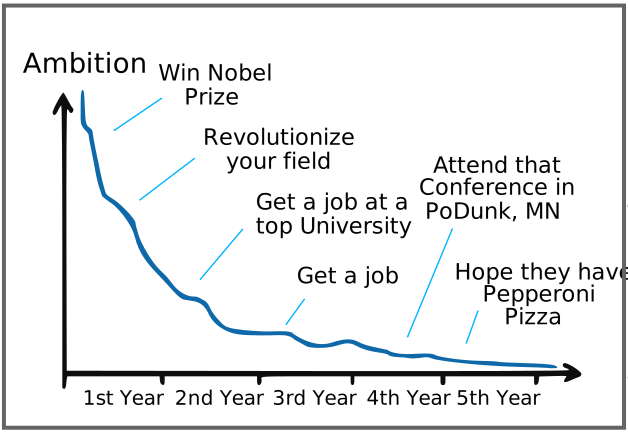
\includegraphics[height=5cm]{bilder/ambition.png}
%\end{figure}

\eject

Wir hoffen, dass alles Wichtige angesprochen wird. Falls ihr noch Fragen, Anregungen oder Kritik habt, könnt ihr euch jederzeit an uns wenden.

Falls ihr euch jetzt fragt, wer oder was die Fachschaft eigentlich ist und was wir außer dem Ersti-Info noch alles machen, dann könnt ihr dies im Kapitel Fachschaft MathPhysInfo nachlesen. \\\\
\noindent Viel Spaß und Erfolg im Studium,\\\\

eure Fachschaft MathPhysInfo


\begin{figure}[b]
\centering
\includegraphics[height=5cm]{bilder/Humor.png}
\end{figure}

%%%%%%%%%%%%%%%%%%%%%%%%%%%%%%%%%%%%%%%%%%%%%%%%%%%%%%%%%%%%%%%%%%%%%%%%%%%%%
\chapter{Vorkurs}
% !TEX ROOT = ../ersti.tex
\section{Vorkurs Informatik}
Da im Informatikstudium in den ersten beiden Semestern verhältnismäßig viele Mathe-Module belegt werden, ist der Mathe-Vorkurs auch allen zukünftigen Infostudierenden zu empfehlen. Er widmet sich einer Einführung in die universitäre Mathematik.
Parallel zu den Mathevorträgen zum Thema „Folgen“, „Gruppen“ und „Kombinatorik“ finden ab dem Mittwoch der zweiten Woche für die Info-Studis Informatik-Vorträge statt. Wo genau ihr diese und alle anderen Veranstaltungen findet, guckt ihr am besten im Internet\footnote{\url{mathphys.info/vorkurs/plan\#info}}.%


\subsection{Programmiervorkurs}
Der Programmiervorkurs richtet sich an alle diejenigen von euch, die noch keinerlei Kenntnisse im Bereich des Programmierens haben und sich im allgemeinen Umgang mit dem Computer unsicher fühlen. Der Kurs findet vom 23. bis 27. September im Mathematikon statt und ist auch für Mathematikerinnen zu empfehlen.

Die Kenntnisse werden in der „Einführung in die praktische Informatik“ (\gls{IPI}, erstes Semester) bzw. spätestens in der „Einführung in die Numerik“ (\gls{Num0}) hilfreich sein. Davon abgesehen ist es nützlich, erste Erfahrungen mit UNIX-artigen Betriebssystemen („Linux“) zu machen, da sie im naturwissenschaftlichen Bereich weit verbreitet sind.

Für den Programmiervorkurs ist aufgrund der begrenzten Plätze im Computer-Pool eine vorherige Anmeldung erforderlich!

% !TEX ROOT = ../ersti.tex
\section{Vorkurs Mathematik}
Der Vorkurs für die Studienanfänger der Mathematik und Informatik wird von der Fachschaft MathPhysInfo organisiert. Er soll helfen, euch den Einstieg in das Studium zu erleichtern. Dazu gibt es vormittags fachliche Vorträge und Übungen und nachmittags alles, was nicht direkt mit Mathe zu tun hat: wichtige Infos zu wechselnden Themen und ein umfangreiches Kennenlern- und Spaßprogramm.
Die Veranstaltungen finden an unterschiedlichen Orten statt, die auf dem Plan im Internet \marginQRsmall{http://mathphys.info/vorkurs/plan\#mathe} unter \url{mathphys.info/vorkurs/plan\#mathe} abzulesen sind. Die Begrüßungsveranstaltung findet am Montag, den 02.10. von um 9 Uhr im Gebäude \gls{INF} 252 (Chemie) in großen Hörsaal statt. Die Informationsvorträge finden täglich 14 bis 15 Uhr im Mathematikon (\gls{INF} 205) im Hörsaal statt.

% !TEX ROOT = ../ersti.tex
\section{Vorkurs Physik}
Der Vorkurs der Physik besteht aus einem Mathematik-Vorkurs der Fakultät für Physik, gelesen von \dozentvorkurs. Seit Einführung des Bachelor wird auch ein Kurs zu Schlüsselkompetenzen angeboten, der zum Bachelor-Programm gehört, jedoch nicht verpflichtend ist. Ihr könnt also bereits durch den Vorkurs eure ersten Credit-Points erhalten. Treffpunkt ist am 25.09.2017 um 9 Uhr im Hörsaal 1 der \Gls{Physik}, \Gls{INF} 308. Die genauen Inhalte des Vorkurses legt der Dozent je nach Kenntnisstand der Hörerschaft fest, wobei das zugehörige Skript\footnote{\url{http://www.thphys.uni-heidelberg.de/~hefft/vk1/}} einen guten Anhaltspunkt bietet.

Einen genauen Plan der Vorkursveranstaltungen und Orte findet man im Internet \marginQR{http://mathphys.info/vorkurs/plan\#physik} unter \url{mathphys.info/vorkurs/plan\#physik}.

Das Rahmenprogramm, welches ihr (ab der zweiten Woche) gemeinsam mit den Mathematikerinnen und Informatikerinnen habt, wird von der Fachschaft MathPhys organisiert und durchgeführt.
% In der ersten Woche findet ein Spiel statt, bei dem ihr die Stadt kennenlernen könnt.
% Mit "der ersten Woche" ist die 2. Woche gemeint!

Den Vorkurs gibt es inzwischen auch als gebundenes Buch (siehe Buchliste). Geht ruhig mal in der ersten Vorkurswoche in die Universitätsbibliothek und leiht es euch sozusagen als Begleitbuch aus. (Vom Kauf möchten wir dennoch abraten.)

% !TEX ROOT = ../ersti.tex
\section{Rahmenprogramm}
\subsection{Wanderungen}
An den Wochenenden -- Sonntag 18.10. und Sonntag 25.10. -- haben wir vor jeweils eine kleine Wanderung unternehmen. Die erste Tour führt auf den Heiligenberg, die zweite auf den Königstuhl -- die beiden Hausberge (Hügel) Heidelbergs. Im Anschluss an die erste Tour werden wir an der Thing-Stätte\footnote{alle Infos hierzu während der Wanderung erfragen} grillen, im Anschluss an die zweite Tour im Schlossgarten picknicken. Bringt euch für das Picknick alles Wichtige selber mit.\\

\noindent\emph{In der Regel treffen wir uns jeweils um 11 Uhr am Bismarckplatz. Corona-bedingt kann es zu Änderungen kommen, die wir euch dann mitteilen.}

\vfill


\eject

\subsection{Spieleabende}
Das Abendprogramm wird spontan entschieden, meist handelt es sich um Gesellschaftsspiele -- bringt auf jeden Fall eigene Spiele mit, was auch immer ihr unter Spielen versteht.

Bisher sind Gesellschaftsspiele super angekommen -- da lernt man sich kennen -- Alternativvorschläge sind natürlich trotzdem immer gern gesehen. Falls euch etwas einfällt, meldet euch doch einfach, schließlich wird der Abend ja für euch veranstaltet.

Auch hier kann es zu Änderungen kommen, wir versuchen euch eine digitale Möglichkeit anzubieten. Nähere Infos kommen noch.

\subsection{Brunch}
Am Samstag den 17. Oktober bereiten wir euch einen wunderschönen, leckeren Brunch im \gls{Mathematikon}, der das beste Frühstück wird, das ihr in euren ersten zwei Wochen bekommen werdet. Bringt bitte euer eigenes Geschirr/Besteck mit, damit wir Plastikquatsch sparen.
Es kann sein, dass diese nicht stattfindet, wir informieren euch rechtzeitig.

\vspace{4cm}

\begin{figure}[h]
\centering
\includegraphics[width=.7\linewidth]{bilder/su_doku.png}
\end{figure}


%%%%%%%%%%%%%%%%%%%%%%%%%%%%%%%%%%%%%%%%%%%%%%%%%%%%%%%%%%%%%%%%%%%%%%%%%%%%%
\chapter{Studiengänge}
\section{Bachelor Allgemein}
Der Bachelor ist in den ersten Semestern sehr stark von Pflichtvorlesungen
geprägt, die kaum Wahlmöglichkeiten lassen. Gerade die ersten zwei Semester
sind in der Regel mit den Grundvorlesungen gut gefüllt. Ab dem dritten Semester
ist es dann aber meist möglich, euren Interessen nachzugehen.
Ein Bachelor lässt sich in drei bis vier Bereiche einteilen: Pflichtbereich,
Wahlpflichtbereich und Übergreifende Kompetenzen. Im Bachelor Physik kommt noch
der Wahlbereich hinzu, in der Informatik ein Anwendungsgebiet.
Der Pflichtbereich dient dazu, euch die Grundlagen eures Fachs beizubringen und
euch mit der fachlichen Methodik vertraut zu machen.  Im Wahlfpflichtbereich
vertieft ihr dann eure Kenntnisse und spezialisiert euch oft auf ein Gebiet. Im
Bereich Übergreifende Kompetenzen geht es um Soft- und Social Skills, aber auch
um fachlich übergreifendes Wissen.  Im Wahlpflichtbereich könnt ihr
schließlich all das einbringen, was euch Spaß macht und nicht durch einen der
anderen Bereiche abgedeckt ist.

Die verschiedenen Veranstaltungen, die ihr während eures Studiums besucht, sind
in sogenannte Module gegliedert. Nach Definition ist ein Modul eine „thematisch
und zeitlich abgeschlossene Lehr- und Lerneinheit“. Ihr müsst euch allerdings
nicht lange mit dieser doch etwas umständlichen Formulierung befassen. Für euch
ist ein Modul nämlich nichts anderes als eine Vorlesung, die meist mit einer
schriftlichen Prüfung abgeschlossen wird, oder ein Seminar, in dem die Prüfung
aus einem Vortrag zu einem der Seminarthemen. Hin und wieder können euch auch
Module begegnen, die aus mehreren Veranstaltungen bestehen. Dann müsst ihr zum
Abschließen des Moduls eben nicht nur eine Prüfung bestehen oder einen Vortrag
halten, sondern eben alle\footnote{rechtlich heißt es zwar „ein Modul, eine
Prüfung“, aber man kann da Ausnahmen machen.} Verstaltungen des Moduls bestehen.

Um den Stoff einer Vorlesung über das Semester hin zu vertiefen, gibt es in
fast allen Vorlesungen jede Woche einen Übungszettel mit Aufgaben zum aktuellen
Thema. Diese Zettel sind einerseits gut, um den Vorlesungsstoff aufzuarbeiten
und anzuwenden, andererseits braucht ihr auf den Zetteln in der Regel 50\% der
Punkte, um überhaupt zur Klausur zugelassen zu werden. Wie genau das dann
funktioniert, wird euch in den einzelnen Vorlesungen am Anfang jedes Semesters
ausführlich erklärt.

Für bestandene Module bekommt ihr dann Leistungspunkte (LP)\footnote{manchmal
auch Credit Points (CP) genannt}, von denen ihr in eurem Studium insgesamt 180
sammeln müsst (mit einigen Bedingungen verknüpft), um euren Bachelor zu
bekommen. Die Anzahl der Punkte, die ein Modul gibt, berechnet sich aus dem
„Workload“ einer Vorlesung. Das ist der Arbeitsaufwand, den eine Vorlesung und
die dazugehörige Übung mit sich bringt. Zum einen Teil ist das also Zeit, die
ihr in der Vorlesung und in den Übungen sitzt, aber auch die Zeit, die ihr für
das Vor- und Nachbereiten der Vorlesung und für das Rechnen des zugehörigen
Zettel braucht. Dabei entspricht ein LP in etwa 30 Stunden Arbeit im Semester,
also gute zwei Stunden pro Woche. Da es natürlich stark von euch abhängt, wie
lange ihr für das alles braucht und wie viel Zeit ihr wirklich investieren
wollt, kann das nur eine grobe Abschätzung sein, ist aber eine gute
Orientierung, wenn ihr überlegt, wie viel ihr euch im Semester aufbürden wollt.

\section{Bachelor Angewandte Informatik}
\sidebar{
    \centering
    \includegraphics[width=3cm]{bilder/cant_sleep_1.png}\\\vspace{13mm}
    \includegraphics[width=3cm]{bilder/cant_sleep_2.png}\\\vspace{13mm}
    \includegraphics[width=3cm]{bilder/cant_sleep_3.png}\\\vspace{13mm}
    \includegraphics[width=3cm]{bilder/cant_sleep_4.png}
}

\subsection{Die ersten Semester}

Im ersten Semester hört ihr die Informatikvorlesungen „Einführung in die Praktische Informatik“ (\gls{IPI}) und „Einführung in die Technische Informatik“ (\gls{ITE}) sowie eine Mathematikvorlesung. Weiterhin ist der „Programmierkurs“ (\gls{IPK}) Pflicht, in dem grundlegende Fertigkeiten in C++ vermittelt werden sollen.

In IPI sollt ihr Programmieren und andere Grundfertigkeiten lernen. Ihr sollt einen Überblick über verschiedene Grundkonzepte der Informatik und Grundkenntnisse in einer oder mehrerer Programmiersprachen bekommen.

ITE soll euch Kenntnisse über den grundsätzlichen Aufbau und die Funktionsweise von Rechnern vermitteln. Ihr lernt Schritt für Schritt, angefangen bei Logik und einfachen Schaltungen, wie ein Prozessor und letztendlich ein ganzer Computer funktioniert.


\subsection{\dots{}Später dann}

In den späteren Vorlesungen werden einzelne Themengebiete eröffnet und vertieft, die Namen der Vorlesungen sprechen zum größten Teil für sich, zum Beispiel „Datenbanken“ (\gls{IDB1}) oder „Betriebssysteme und Netzwerke“ (\gls{BeNe} bzw. IBN).

Außerdem müsst ihr noch ein Proseminar, ein Seminar sowie ein An\-fän\-ger-- und ein Fortgeschrittenen--Praktikum (\gls{AP} und \gls{FP}) machen. Diese unterscheiden sich von Vorlesungen da von der Modulbeschreibung kein Inhaltliches Thema vorgegeben wird sondern lediglich die Veranstaltungsform.

Im Seminar und Proseminar müsst ihr euch zu einem Thema, das zu Beginn zugeteilt wird, genau informieren und dann einen Vortrag halten in dem ihr den weiteren Seminarteilnehmern das Thema erklärt. Natürlich beschäftigt sich ein Seminar immer mit einem zusammenhängenden Themenbereich. Während bei einem Proseminar theoretisch mehr auf die Art der Präsentation geachtet wird, ist es bei dem Seminar vor allem wichtig einen inhaltlich guten Vortrag zu halten. Diese Trennung ist aber meistens gar nicht so klar.

Bei den Praktika bekommt ihr ein Softwareprojekt das ihr, in einer Gruppe von zwei bis drei Personen, innerhalb eines Semesters schreiben sollt. Dabei habt ihr meist viel Freiheit wie ihr euch die Zeit und die Arbeit einteilt, da ihr lediglich zum Semesterende fertig sein müsst. Das AP und FP unterscheiden sich in der Regel nur in ihrer Komplexität.

\subsection{Mathe und so\dots}

Das Informatikstudium in Heidelberg beinhaltet einen in Vergleich zu anderen Universitäten hohen Anteil an Mathematik. Ihr könnt von Anfang an entscheiden, welche Art der Mathematikausbildung ihr erhalten möchtet. Ihr habt die Wahl zwischen mehreren Varianten.

In der ersten Variante hört ihr die Vorlesungen „Lineare Algebra 1“ (\gls{LA}, im 1. Semester) und „Analysis 1“ (\gls{Ana}, im 3. Semester). Alternativ könnt ihr als Ersatz für die LA 1 und die Ana 1 im ersten und zweiten Semester die Veranstaltungen „Mathematik für Informatiker 1“ (\gls{MafIn} bzw. IMI, entspricht etwa LA 1) und „Mathematik für Informatiker 2“ (ersetzt Ana 1) hören. Diese Vorlesungen soll den Informatikstudis speziell die Mathematikkenntnisse vermitteln, die sie in ihrem späteren Studium brauchen werden. Diese Veranstaltung bemüht sich solide Mathematikgrundlagen zu vermitteln und versucht einen Bezug zur Informatik herzustellen. Welche Vorlesung ihr hören solltet, wird im \autoref{mafin} diskutiert.

Hinzu kommen noch die Vorlesung „Einführung in die Numerik“ (\gls{Num0}) und eins der drei Module „Analysis 2“, „Mathematische Logik“ oder „Einführung in die Wahrscheinlichkeitstheorie und Statistik“ (\gls{WTheo0}). Dazu dürft ihr noch bis zu einem Mathematikmodul belegen, das ist aber freiwillig und ihr könntet genauso gut ein Informatikmodul stattdessen belegen,

Die Mathematikmodule unterscheiden sich stark von der Schulmathematik, unterschätzt den Aufwand für die Vorlesungen nicht! Wenn ihr schon wisst, dass ihr euer Informatikstudium mathematisch ausrichten und weitere Mathematikmodule hören wollt und euch vielleicht später sogar im wissenschaftlichen Rechnen spezialisieren möchtet, ist die Variante mit LA 1 und Ana 1 empfehlenswert.

\subsection{Programmieren. Und dann\dots}

\sidebar{
    \centering
    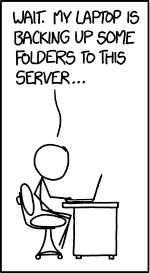
\includegraphics[width=3cm]{bilder/backing_up_1.png}\\\vspace{5mm}
    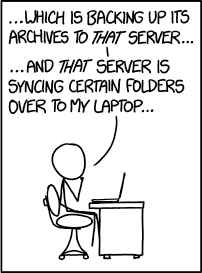
\includegraphics[width=3cm]{bilder/backing_up_2.png}\\\vspace{5mm}
    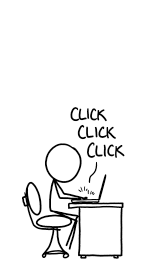
\includegraphics[width=3cm]{bilder/backing_up_3.png}\\\vspace{5mm}
    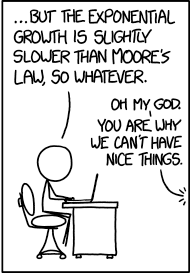
\includegraphics[width=3cm]{bilder/backing_up_4.png}
}

Programmieren ist eine wichtige Fertigkeit. Und die werdet ihr nur teilweise an der Uni lernen. Im IPK und in der IPI wird versucht, euch die Konzepte näher zu bringen und in den Übungsaufgaben werdet ihr selber kleinere Sachen programmieren müssen.

Es gibt eine enorme Anzahl an Programmiersprachen und die meisten haben ihre Daseinsberechtigung: um praktische Probleme zu lösen, akademisches Interesse oder auch Unterhaltung. Es gibt diverse Paradigmen, nach denen Programmiersprachen konzipiert sind und an der Uni werdet ihr nur die wenigsten kennen lernen. Auch solltet ihr das System kennen, auf dem ihr arbeitet: solide Kenntnisse von unixoiden Systemen, wie Linux und OSX, sind immer Gold wert.

Die Uni hilft aber durchaus: Die IPI vermittelt unter anderem grobe Programmierkenntnisse, es gibt den richtigen „Programmierkurs“ IPK, der auch Pflicht ist und zu Num0 gibt es praktische Übungen, in denen ebenfalls programmiert wird. Eigeninitiative ist aber dennoch wichtig, mit interessanten Projekten macht das aber auch enorm viel Spaß.


\subsection{Anwendungsgebiet}

Neben dem ganzen Informatik-Kram habt ihr noch ein Anwendungsgebiet. Das ist nicht (wie es sich vielleicht anhört) eine Informatik-Anwendung, sondern einfach ein anderes Fach, in dem ihr einige Veranstaltungen (24 \gls{LP}) hören müsst.

Im Modulhandbuch sind zwar nur einige wenige Fächer als mögliches Anwendungsgebiet aufgelistet, aber das heißt nicht, dass ihr euch nichts anderes anrechnen lassen könnt.

Wenn ihr euch also für andere Fächer mehr interessiert, dann könnt ihr in Absprache mit dem Prüfungsausschuss mit Sicherheit auch dieses Fach hören.

In den meisten Fächern sind die Module, die ihr hören sollt bereits vorgeschrieben. Für gewöhnlich sind dies die Grundmodule des jeweiligen Faches, oft habt ihr jedoch trotzdem einige Wahlmöglichkeiten.


\subsection{Orientierungsprüfung}

Auch in Informatik gibt es eine sog. Orientierungsprüfung. Die besteht darin, dass ihr bis spätestens zum Ende des 3. Semesters die Vorlesung „Einführung in die Praktische Informatik“ bestanden haben müsst.


\subsection{Prüfungen: wie und wieso?}

Zum Thema Prüfungen und Prüfungswiederholungen: Um in den Vorlesungen Leistungspunkte (meisten mit \gls{LP} oder \gls{CP} abgekürzt) zu bekommen, sprich das Modul abzuschließen, müsst ihr am Ende in den meisten Fällen eine schriftliche Prüfung bestehen. Die genauen Modalitäten, um überhaupt für die Prüfung zugelassen zu werden, legen die DozentInnen jeweils am Anfang des Semesters fest. Informiert euch unbedingt genau, worin die bestehen! Meist müsst ihr am Ende nur im Mittel 50 oder 60 Prozent der Punkte auf den Übungszetteln erreichen, manchmal ist aber auch gefordert, dass jeder Übungszettel bearbeitet wurde.

Ihr solltet euch auch bei jeder Veranstaltung genau darüber informieren, was genau \emph{eine} Prüfung beinhaltet (z.\,B.\ Bestehen von einer von zwei Klausuren). Insbesondere der letzte Teil ist wichtig, denn ihr könnt Prüfungen grundsätzlich zweimal versuchen. Je nach Veranstaltung und Dozent/in \emph{können} zwei Klausuren als eine Prüfung zählen, müssen aber nicht -- dann würde jede geschriebene Klausur als ein Prüfungsversuch gelten. Wenn ihr aus Gründen, die ihr nicht zu verantworten habt (wie krank sein), nicht an einer \emph{Prüfung} teilnehmen konntet, bekommt ihr entsprechend einen Ausweichtermin. Aber keine Panik -- auch wenn ihr in einer Vorlesung zum zweiten Mal die Prüfung nicht bestanden haben solltet, seid ihr noch nicht exmatrikuliert: In bis zu vier Fällen dürft ihr auf Antrag Prüfungen auch ein zweites Mal wiederholen, dies gilt aber nicht für die Orientierungsprüfung und für die Bachelorarbeit.

Denkt dran: Eine Klausuranmeldung ist eine Anmeldung zu einer Prüfung. Wenn ihr euch sicher seid, sie nicht zu bestehen, überlegt euch lieber zweimal, ob ihr euch anmeldet. Das Schöne an eurem Studiengang ist, dass die Noten der Grundpflichtmodule (IPI, IPK, ITE, LA 1 und Ana 1) nicht in eure Abschlussnote zählen, das heißt, dass auch wenn die ersten Semester mit der ganzen Mathematik vielleicht etwas hart sind, eure Abschlussnote darunter nicht unbedingt zu leiden hat.

\marginpar{
	\centering
	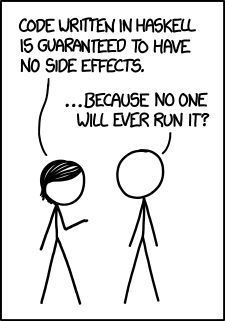
\includegraphics[width=3.5cm]{bilder/haskell.png}
}

\vspace{-\parskip}

\section{Mathematik 100\%}

\subsection{Das erste und zweite Semester}

In den ersten zwei oder drei Semestern hört ihr eure Grundvorlesungen und einige Einführungsvorlesungen. Die Grundvorlesungen sind die „Lineare Algebra“ 1 und 2 (\gls{LA}), in denen ihr hauptsächlich Abbildungen zwischen Vektorräumen betrachtet, und „Analysis“ 1 und 2, sowie „Höhere Analysis“ (\gls{Ana}). Dort behandelt ihr Grenzwerte mit allem, was folgt, das heißt Differential- und Integralrechnung.

Auf der Webseite der Fakultät findet ihr nochmal eine Auflistung\footnote{\url{https://www.mathematik.uni-heidelberg.de/modellstudienplaene.html}} wie euer Studium aufgebaut ist. Auch das sind nur Vorschläge, wie ihr euer Studium im Endeffekt einteilt, bleibt natürlich euch überlassen.

\subsubsection{Orientierungsprüfungen}

Orientierungsprüfungen sind Prüfungen, die bis Ende des dritten Semesters bestanden sein müssen. In der Mathe sind das Ana 1 und LA 1 für den 100\%-Bachelor, bzw. LA 1 für 50\%-Bachelor. Diese Vorlesungen müssen also im ersten Semester gehört werden. Sollte man im ersten Anlauf, das heißt in der ersten Klausur und in der Nachklausur nicht bestehen, ist das noch lange kein Weltuntergang. Ihr seid damit nicht die Ersten und nicht die Letzten an der Uni und sicher auch nicht die Einzigen in eurem Semester. Es fallen in manchen Jahren 50\%, mal mehr, mal weniger, durch diese Klausuren durch. Macht euch deshalb also keinen Kopf! Ihr habt dann im WS darauf noch einen Versuch, bestehend aus Klausur und Nachklausur. Der muss dann aber klappen, da euch sonst die Exmatrikulation droht.

\subsubsection{Einführungsvorlesungen}

Die Einführungsvorlesungen bestehen aus der „Einführung in die praktische Informatik“ (\gls{IPI}), „Einführung in die Numerik“ (\gls{Num0}) und „Einführung in die Wahrscheinlichkeitstheorie und Statistik“ (\gls{WTheo0}). In allen Vorlesungen müsst ihr Übungszettel lösen, die dazu dienen, den Stoff zu vertiefen. Ihr habt dann zu jeder Vorlesung Übungsgruppen und Tutorinnen, die nicht nur eure Zettel korrigieren und sie mit euch besprechen, sondern vor allem dazu da sind, euch zu helfen. Tutorinnen werden dafür bezahlt, eure Fragen zu beantworten, egal wie dumm sie euch in dem Moment vorkommen, und machen das auch gerne. Auch die anderen Studis verstehen meist nicht mehr als ihr, sehr wahrscheinlich haben sie ähnliche Fragen. Sucht euch am besten am Anfang eine Gruppe von Kommilitoninnen, mit denen ihr gut rechnen und überlegen könnt, damit ihr die Zettel nicht alleine bearbeiten müsst. Abgeben sollt ihr sie auch nicht alleine, sondern im Allgemeinen zu zweit.

Zusätzlich kann im zweiten Semester ein Proseminar besucht werden. Das Proseminar setzt eine aktive Teilnahme voraus und wird mit einem mündlichen Vortrag abgeschlossen, eventuell mit zusätzlicher schriftlicher Ausarbeitung. Der Vortrag ist eine sehr gute Möglichkeit \LaTeX\ zu lernen. \LaTeX\ ist ein Programm, um PDF-Dokumente zu schreiben, ihr werdet es in eurem Mathestudium noch häufig brauchen und wie heißt es so schön: Früh übt sich, wer ein Meister werden will \textit{(Schiller)}.

\subsubsection{Ist Mathe wirklich richtig für mich?}

In den ersten beiden Semestern kann es passieren, dass eure Noten nicht so gut sind, wie ihr das vielleicht gerne hättet oder aber gewohnt seid. Das ist aber noch lange kein Weltuntergang und auch noch kein Grund, das Studium abzubrechen, wenn ihr Spaß an Mathematik habt. Mathematik an der Uni ist etwas ganz anderes als die Mathematik, die man aus der Schule kennt. Es wird auch gerne die Tatsache unterschätzt, dass man plötzlich in einer ganz neuen Situation ist, eine für die meisten fremde Stadt, neue Leute, ein ganz anderes System als die Schule. Man muss sich erstmal an die geänderten äußeren Umstände gewöhnen und das braucht Zeit. Auch die Klausuren sind nicht so schlimm, wie es einem am Anfang vorkommen mag. Ihr habt im Regelfall eine zweite Chance, wenn ihr durch die erste durchfallt. Sollte auch der zweite Anlauf nicht klappen, dann könnt ihr die Vorlesung im nächsten Jahr noch einmal hören. Es ist also nichts verloren. Verzweifelt nicht zu schnell an der noch sehr ungewohnten Uni-Mathe, ihr werdet euch schnell daran gewöhnen. Ebenfalls wird aus LA 1 und 2 sowie Ana 1 und 2 auch nur die jeweils bessere Lineare-Algebra- und Analysis-Note in eurem Bachelor berücksichtigt.

Wenn ihr sonst über irgendetwas stolpert, gibt es immer noch die Fachschaft, die euch gerne weiterhilft. Ihr könnt entweder persönlich bei uns vorbei kommen oder eine Mail schreiben. Wir versuchen dann, euch zu helfen, wo es nur geht.

\subsection{Alle weiteren Semester}

Der weitere Verlauf des Studiums kann von jeder ganz individuell gestaltet werden. Man kann sich dabei nach einem der Stundenpläne, die auf der Homepage der Fakultät\footnote{\url{https://www.mathematik.uni-heidelberg.de/modellstudienplaene.html}} zu finden sind, richten. Bei der Frage, welche Vorlesungen und Veranstaltungen ihr belegen müsst und könnt, helfen euch Modulhandbuch, Prüfungsordnung und Homepage der Fakultät.

\subsection{Prüfungsordnung}

In der Prüfungsordnung (PO) findet ihr alle wichtigen Informationen darüber, welche Veranstaltungen gehört werden müssen, welche Prüfungen wann und wie abgelegt werden müssen und wie euer Studium sonst geregelt ist. In der Prüfungsordnung könnt ihr nachschlagen, welche Pflicht- und Wahlpflichtveranstaltungen es gibt und wie viele und welche Wahlpflichtveranstaltungen gehört werden müssen (Anlage 1 und 2).  Im Modulhandbuch findet ihr kurze Beschreibungen der Veranstaltungen und welche Vorkenntnisse für sie empfohlen werden. Neben Pflicht- und Wahlpflichtmodulen gibt es noch das Anwendungsgebiet und fachübergreifende Kompetenzen. Über letztere braucht ihr euch keine großen Sorgen zu machen, die hat man meist schneller als man denkt. Möglichkeiten sind hier Praktika, Auslandssemester, Sprachkurse, die das Zentrale Sprachlabor der Universität Heidelberg anbietet, Vorlesungen anderer Fächer und so weiter. 8 der 20 Leistungspunkte für fachübergreifende Kompetenzen sind bereits in andere Veranstaltungen integriert. In Anlage 3 der PO findet ihr mehr Informationen darüber, wie und wann ihr diese Leistungspunkte erwerbt.

\subsection{Anwendungsgebiet}

Zusätzlich zum puren Mathematik-Studium habt ihr das Anwendungsgebiet, was ein Fach eurer Wahl sein kann. In der Prüfungsordnung gibt es aber nur für die Fächer Informatik, Physik, Astronomie, Biologie, Chemie, Wirtschaftswissenschaften und Philosophie eine feste Regelung. Nach Rücksprache mit dem Prüfungsausschuss können jedoch auch andere Fächer angerechnet werden. Habt ihr zum Beispiel ein Studium vorher abgebrochen, kann das oft als Anwendungsgebiet angerechnet werden. Die meisten der oben genannten Fächer fangen laut Musterstudium in eurem dritten Semester an, die interessanten Informatikvorlesungen sind dagegen im Sommersemester. Niemand wird euch daran hindern, euer Anwendungsgebiet schon im ersten Semester zu beginnen, unterschätzt jedoch die Arbeitsbelastung des Grundstudiums nicht.

\subsection{Am Ende Bachelor?}

Ganz am Ende erwarten euch dann noch ein weiteres Seminar, welches häufig als Grundlage für die Bachelorarbeit verwendet wird, und zuletzt die Bachelorarbeit und das zugehörige Bachelorseminar, in dem ihr in der Regel die Arbeit präsentiert.


% !TEX ROOT = ../ersti.tex
\section{Bachelor Physik}

\subsection{Erstes Semester}

Das erste Semester ist, verglichen mit späteren Semestern, sehr stark durchstrukturiert, was euch den Wechsel von der Schule an die Uni erleichtert, jedoch auch nicht besonders viele Freiheiten lässt.  Allgemein werdet ihr bis ins vierte Semester im Pflichtprogramm je eine „Experimentalphysik“ (\gls{Ex}) und eine „Theoretische Physik“ (\gls{Theo})\footnote{Die Abkürzung „Theo“ kann zu Verwirrungen mit Informatikern führen, da diese das als „Theoretische Informatik“ verstehen.} Vorlesung besuchen, wobei im fünften Semester noch die Ex 5 folgt. Zusätzlich dazu hört ihr an Mathe im ersten Semester die „Lineare Algebra 1“ (\gls{LA}) und wenn ihr wollt auch die „Analysis 1“ (\gls{Ana}); aber zur Mathe später mehr.

Das ganze Semester über werdet ihr jede Woche in jeder Vorlesung, die ihr hört, einen Übungszettel bekommen, den ihr dann auf die nächste Woche lösen sollt. Diese dienen zum Einüben des in den Vorlesungen behandelten Stoffes und zugleich häufig als Klausurzulassung. Man benötigt meistens insgesamt 50 - 60 \% der Gesamtpunktzahl auf allen Zetteln, aber wenn es nur um ein paar Punkte geht, sind die Tutoren meistens kulant. Wenn euer Tutor den Eindruck hat, ihr verschwendet nicht nur einen Prüfungsversuch mit der Klausur, lässt er euch meistens zu. Macht euch darum aber erstmal keinen Kopf, wenn man am Ball bleibt, ist das überhaupt kein Problem, ihr müsst sie ja nicht alle alleine lösen.

\subsection{Orientierungsprüfung}

Die Orientierungsprüfung ist eine Prüfung, die ihr bis zum Ende des 3. Semesters bestehen müsst, um weiterhin Physik studieren zu dürfen. Im Bachelor Physik ist dies die ganz normale Klausur in der Ex 1. Dort werden meist sehr schulnahe physikalische Grundlagen der Mechanik behandelt. Macht euch also keine Sorgen. Das schafft ihr!

\subsection{Basiskurs}

Der Basiskurs beginnt, wie ihr wahrscheinlich schon wisst, in der letzten Vorkurswoche und soll euch den Einstieg in das Studium erleichtern. Dabei werden euch sogenannte Schlüsselkompetenzen beigebracht, die euch unter anderem in Zeitmanagement, Literatursuche und das Textsatzsytem \LaTeX{} einführen. Auch wenn ihr vermutlich schon einiges davon kennt, ist es doch ganz nett, nochmal alles kompakt zu sehen und vor allem dabei neue Menschen und vielleicht auch spätere „Zettelpartnerinnen“ kennenlernen zu können. Leider ist die Qualität des Kurses oft stark abhängig von eurer Tutorin. Ihr müsst also für euch bestimmen, wie viel ihr aus diesem Kurs mitnehmt. Bedenkt, die Tutorin bekommt Geld für diesen Kurs, ihr dürft also auch etwas von ihr erwarten. 

\subsection{Analysis vs. Höhere Mathematik für Physiker}
Ihr habt zwei Möglichkeiten, die für das Studium benötigte Analysis zu erlernen.
In der ersten Variante hört ihr im zweiten Semester die Vorlesung „Höhere Mathematik für Physiker 2“\footnote{Es gibt keine „Höhere Mathematik für Physiker 1“, weil die Vorlesungen parallel zur Ana 2 und Ana 3 laufen.} (\gls{HoMa}) und im dritten Semester „Höhere Mathematik für Physiker 3“. Alternativ dazu könnt ihr im zweiten Semester Ana 2 und im dritten Semester Ana 3 hören. Falls ihr euch dafür entscheidet, bietet es sich an, zusätzlich im ersten Semester die Vorlesung Ana 1 zu hören. Diese Problematik wird im \autoref{mathephysik} weiter diskutiert.

\subsection{Weiteres Studium}

Euer weiteres Studium sieht, wie oben kurz angedeutet, so aus, dass ihr immer ein Grundgerüst an Vorlesungen habt und euch darum herum andere Vorlesungen und Seminare selbst auswählen könnt. Die Experimentalphysikvorlesungen sind bis zum fünften Semester und die theoretischen bis zum vierten Semester Pflicht. Hinzu kommen im zweiten und dritten Semester entweder die HöMa 2 und 3, oder die Ana 2 und 3. Ansonsten seid ihr jedoch bis auf ein Pflichtseminar, das ihr aus einem relativ großen Topf an Seminaren auswählen könnt und den Pflichtpraktika frei alles zu hören, was euch so in den Sinn kommt. Ihr müsst einzig darauf achten, dass ihr in den einzelnen Bereichen ausreichend „Punkte sammelt“: Im Wahlpflichtbereich sind das 14 \gls{LP}, bei den Übergreifenden Kompetenzen 19 \gls{LP} und im Wahlbereich bis zu 17 \gls{LP}. Nutzt frühzeitig die Gelegenheit Veranstaltungen zu besuchen, die euch interessieren, dann macht das Studium gleich doppelt so viel Spaß!

\begin{figure}
	\centering
	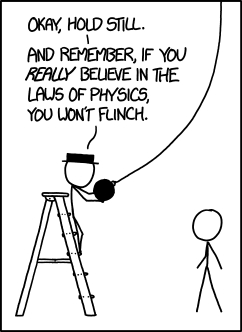
\includegraphics[width=.5\linewidth]{bilder/laws_of_physics.png}
\end{figure}

\subsection{Wahlbereich, Wahlpflichtbereich und Übergreifende Kompetenzen}

Im Laufe Eures Bachelorstudiums müsst ihr ggf. ein oder zwei Wahlfächer belegen, welche ihr aus einem recht weit gefächerten Angebot wählen könnt. Diese Wahlfächer müssen auch nicht zwingendermaßen aus Bereichen der Physik kommen, sondern können z.B. Mathe, Chemie oder Philosophie sein. Was ihr alles für Möglichkeiten habt, könnt ihr genauer in der Prüfungsordnung nachlesen und selbst Fächer, die dort nicht aufgezählt sind, lassen sich möglicherweise nach Absprache mit dem Prüfungsausschuss auch anrechnen lassen.\\

Der Wahlpflichtbereich besteht, im Gegensatz zum Wahlbereich und den Übergreifenden Kompetenzen, aus vertiefenden oder weiterführenden Physikveranstaltungen. Schaut doch einfach in das Vorlesungsverzeichnis im LSF und sucht euch interessante Vorlesungen oder auch Seminare aus. Besonders Seminare können viel Spaß machen, da diese zwar oftmals viel selbstständiges Arbeiten verlangen, aber oft auch forschungsnäher sind als Vorlesungen. Zudem findet ihr auch Anregungen dazu in der Prüfungsordnung und im Modulhandbuch.\\

Der Bereich Übergreifende Kompetenzen soll euch ein wenig dazu bewegen fachunabhängige Kompetenzen zu erlernen. Darunter fallen der mathematische Vorkurs, der Basiskurs, sowie alle als „Überfachliche Kompetenzen“ gekennzeichneten Module der Mathematik, Informatik und den Naturwissenschaften. Außerdem lassen sich oft nach Rücksprache mit dem Prüfungssekretariat auch weitere Veranstaltungen anrechnen lassen, wie zum Beispiel Sprachkurse, Programmierkurse, usw.\\

Allgemein gilt: Versucht, möglichst früh Dinge aus Gebieten, die euch wirklich interessieren, zu hören; denn das sind die Fächer die euch auch wirklich Spaß machen und ihr erlangt ein möglichst breites, und vor allem tiefes Wissen, welches euch bei eurer Bachelorarbeit und vermutlich auch sonst zugutekommt.

\subsection{Prüfungen und Noten}

Es wird euch sicher freuen zu hören, dass eine nicht bestandene Klausur nicht gleich das Ende für euer Studium bedeutet. Im Grunde ist die Wiederholungsregelung sogar recht studifreundlich; so habt ihr in jedem Modul zwei Versuche, wobei in der Regel ein Versuch aus einer Klausur und, wenn nötig, der dazugehörenden Nachklausur besteht. Darüber hinaus habt ihr für euer Studium noch zwei sogenannte Joker, die euch jeweils einen dritten Versuch geben, falls die zwei regulären nicht reichen sollen (dies gilt nicht für eure Orientierungsprüfung, welche die Prüfung in der Ex 1 darstellt). Darüber hinaus ist für euch recht interessant, dass es die Möglichkeit gibt, zwei Noten aus unterschiedlichen Bereichen der tendenziell schlechteren Pflichtmodule zu streichen. Macht euch also nicht zu viele Gedanken darüber, wenn eure Noten zunächst nicht ganz so gut sind. Auch könnt ihr jederzeit zusätzlich gehörte Module in den Zusatzqualifikationenbereich verschieben, wenn ihr diese nicht benötigt, euch entsteht also kein Nachteil dadurch, dass ihr mehr hört, als ihr müsst.\\

Sonst ist noch zu erwähnen, dass ihr, um in Heidelberg in den Master zugelassen zu werden, eine Bachelornote von 2,9 oder besser braucht. Das war bisher, so wurde uns versichert, aber noch nie ein Problem, für Heidelberger Studis, der Notenschnitt lag im Bachelor bei etwa 1,7. %Gilt das immer noch?

\subsection{Prüfungsordnung und Modulhandbuch}

Immer dann, wenn sich euch Fragen zu eurem Studium stellen oder ihr euch einfach über den weiteren Studienverlauf informieren wollt, sind die ersten Anlaufstellen die Prüfungsordnung und das Modulhandbuch. In der Prüfungsordnung ist formal geregelt, wie der Studienablauf, die Prüfungen und die Anrechenbarkeit von Modulen aussehen. Das Modulhandbuch wiederum ist im Großen und Ganzen eine Auflistung der in der Physik (und benachbarten Gebieten) angebotenen Veranstaltungen. Zurzeit findet ihr beide Dokumente auf der Hauptseite des Bachelors Physik. Leider ist das Modulhandbuch oft nicht ganz aktuell, falls euch Verbesserungen auffallen, meldet euch einfach bei uns.\\

Ansonsten könnt ihr auch gerne zu uns in die Fachschaft auf eine Tasse Kaffee oder Tee vorbeikommen. In vielen Fällen können wir euch auch weiterhelfen.

\begin{figure*}[h]
    \centering{
    \includegraphics[width=\textwidth]{bilder/purity.png}
}
\end{figure*}

% !TEX ROOT = ../ersti.tex

\section{Der 50\%-Bachelor (Lehramt)} % Dereinst "Lehramt allgemein"
\label{lehramt_allg}

Lehramtsstudiengang, Staatsexamen, Referendariat -- so ging es vor 2015 zurück an die Schule. Die ersten beiden Schritte haben sich nun verändert, denn die Umstellung der Studiengänge in Deutschland auf das zweistufige Bachelor-Master-System macht auch vor dem Lehramt in Baden-Württemberg nicht halt. Und daher heißt es jetzt: Doppel-Fachbachelor, Master of Education, Referendariat. Andernorts heißt es manchmal auch: Bachelor of Education, Master of Education, Referendariat. Das zweite Konzept versucht, das alte Lehramtsstudium soweit wie möglich zu erhalten, während in Heidelberg mit dem heiEDUCATION-Konzept eine Umstellung auf das Erste vorgenommen wird -- mit dem Nebeneffekt, dass es künftig auch möglich sein wird, Informatik, Mathematik und Physik als 50\%-Bachelorstudiengang zu studieren.

\subsection{Praktische Tipps für Lehramtsstudierende}
In einem Lehramtsstudium wird es sicherlich auch vorkommen, dass ihr Veranstaltungen in der Altstadt besuchen werdet, vor allem wenn sich euer Zweitfach in der Altstadt befindet. Deshalb solltet ihr beim Zusammenstellen eures Stundenplans darauf achten, genügend Zeit einzuplanen, um rechtzeitig in der Altstadt (oder im Feld) anzukommen.

Es gibt prinzipiell zwei Möglichkeiten um zwischen dem Neuenheimer Feld und der Altstadt zu pendeln. Zum einen könntet ihr mit dem Bus Nr. 31/32  fahren zum anderen mit dem Fahrrad. In beiden Fällen ist es zu empfehlen, mit einer halben Stunde von Hörsaal zu Hörsaal zurechnen. Allerdings ist das Fahrrad eindeutig das zuverlässigere Verkehrsmittel. Mehr dazu findet ihr unter dem Abschnitt Verkehrsmittel in Heidelberg. 
Ein weiterer Tipp ist, dass ihr euch genügend Zeit zum Zettelrechnen in den Stundenplan einplant, da man in jeder Mathematik-, Informatik- und Physikvorlesung Zettel erhält. Gemeinsam rechnen sich die Zettel deutlich besser. 

Außerdem wird es vorkommen, dass sich gerade bei fakultätsfremden Fächern einzelne Veranstaltungen überschneiden. Genauso kann es vorkommen, dass der Arbeitsaufwand der vorgesehenen Module der beiden Fächer in einem Semester kaum zu leisten ist. Dann solltet ihr keine Scheu haben, den Stundenplan nicht vollständig nach dem Studienverlaufsplan zu gestalten. Sollten dabei Probleme auftauchen, könnt ihr euch Hilfe bei den jeweiligen Fachstudienberaterinnnen suchen.


\subsection{heiEDUCATION}

Das Konzept heiEDUCATION ist von Universität und Pädagogischer Hochschule (PH) Heidelberg gemeinsam entwickelt, um „Heidelberg zu einem Ort exzellenter Lehrerbildung auszubauen“\footnote{\url{https://hse-heidelberg.de/ueber-uns/heieducation}}. Exzellente Lehrerbildung bedeutet dabei folgendes:

Lehramtsstudierende absolvieren zunächst parallel zwei 50\%-Ba\-che\-lor\-stu\-di\-en\-gän\-ge an der Universität Heidelberg. Diese Studiengänge haben fast keinen Lehramtsbezug, lediglich vereinzelte Veranstaltungen für Fachdidaktik und Bildungswissenschaften können belegt werden. Vorgesehen ist, dass man im 6. Semester in einem der beiden Fächer eine Bachelorarbeit schreibt. Während diesem Studium lernt ihr also alle nötigen fachlichen Kompetenzen für das Lehramt.

Anschließend kann man wahlweise auf den „Master of Education“ oder einen Fachmaster in einem der beiden Fächer wechseln. Der „Master of Education“ wird von der Universität und der PH gemeinsam angeboten und soll die notwendigen Kompetenzen für das Unterrichten vermitteln. Diese sogenannte „Polyvalenz“ hat den Vorteil, dass Lehramtsstudierende bis zum 6. Semester Zeit für die Entscheidung zwischen Fach- und Lehramtsausbildung haben, und die 50\%-Bachelorstudiengänge eine interessante Option für Studierende bieten, die an zwei Fächern großes Interesse haben.

Da dieses neue Konzept von denen, die die Umstellung zu verantworten haben, reichlich positiv gesehen wird, sollen an dieser Stelle einige skeptische Worte nicht fehlen:

Die Idee, sich nach einem Bachelor noch entscheiden zu können, hört sich in der Theorie sehr schön an. In der Praxis ist es sehr fachabhängig, wie gut das funktioniert. In einigen Fächern ist die Zulassung zum Fachmaster nur unter Auflagen (d.h. ihr müsst einige Module des 100\% Bachelors im Master  nachholen) möglich. Falls ihr euch also für einen Fachmaster entscheidet seid euch dessen vorher bewusst. 
Ein weiterer Nachteil des 50-50 Bachelors ist, dass das Praxissemester erst sehr spät im Studium verankert ist (momentan im 2. oder 3. Mastersemester). Vorher erhaltet ihr nur im Rahmen des Orientierungspraktikums einen Einblick in den Schulalltag. Auch werdet ihr in euren ersten Semestern kaum auf eure spätere Berufspraxis vorbereitet. Sicherlich ist ein tiefes Verständnis von Inhalten auch jenseits des Schulstoffes wichtig, um später an Schulen gut unterrichten zu können. Doch die tatsächliche Planung von Unterricht, der Schritt vom eigenen Verständnis von Inhalten hin zur Fähigkeit, anderen das Verständnis von Inhalten zu ermöglichen, geschieht in diesem Konzept erst spät. Daher der Appell an all diejenigen, die sich am liebsten schon morgen vor eine Schulklasse stellen und unterrichten würden: Habt Geduld, beißt euch durch und genießt die beiden Praktikas, die ihr im Bachelor habt!

\subsection{Bachelor of Everything\dots}

\dots oder zumindest mal in zwei Fächern gleichzeitig: Einer der Vorteile dessen, wie in Heidelberg das Lehramt umgestellt wurde, ist die hinzugewonnene Möglichkeit, zwei Fächer zu einem Bachelorstudiengang zu kombinieren („Doppelbachelor“) und sich damit für beide Fach-Mas\-ter\-stu\-di\-en\-gän\-ge zu qualifizieren. Zum einen hat man so weitere zwei bis drei Jahre Zeit, sich zwischen den Gebieten zu entscheiden. Zum anderen kann man diesen Studiengang wählen, wenn man zum Ziel hat, an den Grenzflächen zweier Wissenschaften zu arbeiten. Physikalische Chemie, Wissenschaftliches Rechnen und Mathematische Physik sind hier gute Beispiele.

Es muss allerdings darauf hingewiesen werden, dass man sich die größere fachliche Breite auf Kosten der Spezialisierung in den Fächern aneignet. Das kann je nach Fach bedeuten, dass man im Fachmaster später noch Grundlagen aufholen muss, um dieselbe fachliche Tiefe zu erreichen wie die 100\%-Bachelor-Studierenden. Dazu kommt, dass man nur eine Bachelorarbeit schreibt, für die man zwischen den Fächern wählen muss. Teilweise ist an diese Wahl die Zulassung für den Fach-Master geknüpft, teils treffen Fächer Einschränkungen auf bestimmte Fächerkombinationen. Es ist für Studierende des Doppelbachelors daher besonders wichtig, schon frühzeitig sich über die formalen Regelungen in ihren Fächern zu informieren. Dies könnte beispielsweise eine überblicksartige Lektüre der Prüfungsordnungen sein. Auch die Hinweise für die Fächer Informatik, Mathematik und Physik in den folgenden Abschnitten sind vermutlich hilfreich, doch es können dort natürlich nicht alle möglichen Fächerkombinationen diskutiert werden.


%TODO: \subsection{Immatrikulation für das Lehramtsstudium}
% -- davon habe ich keine Ahnung...
%
% Früher stand da mal:
% \subsection{Immatrikulation für das Lehramtsstudium}
%
% Grundsätzlich immatrikuliert man sich im Staatsexamensstudiengang Lehramt
% immer in mindestens zwei Hauptfächern. Gegebenenfalls kann nach der
% Zwischenprüfung in den Hauptfächern noch ein drittes Fach -- ein sogenanntes
% Erweiterungsfach -- hinzukommen.
%
% Aber Vorsicht! Manche Fächer können nicht auf Lehramt studiert werden, andere
% Fächer nur in bestimmten Kombinationen. Obwohl das Studierendensekretariat darauf
% achten sollte, kommt es immer wieder vor, dass Leute mit „falschen“
% Kombinationen immatrikuliert werden. Seht auf jeden Fall nochmal selber nach:
% Welche Fächerkombinationen in Baden-Württemberg auf Lehramt studiert werden
% können, entnehmt ihr einer Tabelle des Kultusministeriums, die ihr bei
% verschiedenen Beratungsstellen (meist auch online auf deren Webseite) einsehen
% könnt: Es gibt für jedes Fach eine eigene Lehramtsberatung sowie eine zentrale
% Beratung für Lehramtsstudierende durch das Oberschulamt; für
% rechtsverbindliche Auskünfte sollte man sich an letztere wenden.
%
% \emph{Achtung:} In anderen Bundesländern gelten andere Regelungen!
%
%
% Zur Immatrikulation für einen Lehramtsstudiengang muss eine Bescheinigung über
% die Ableistung eines sogenannten Orientierungspraktikums vorgelegt werden.
% Sofern diese noch nicht vorliegt, kann sie aber für eine begrenzte Zeit noch
% nachgereicht werden. Die konkrete Frist orientiert sich meist an den sonstigen
% Fristen der Immatrikulation, lest hierzu am besten auf der Seite des
% Studierendensekretariats nach oder ruft dort an (06221 -- 54\,54\,54).

\subsection{Lehramtsoption}
Aber Vorsicht! Manche Fächer kann man auf 50\% studieren, sie sind aber nicht auf Lehramt studierbar. Somit sollte man bei seiner Fächerwahl darauf achten, dass beide Fächer auf Lehramt studierbar sind. Dies findet man zum Beispiel auf dieser Seite\footnote{\url{http://www.uni-heidelberg.de/studium/interesse/faecher/index.html}} heraus. Die Lehramts\-option wird durch ein „LO“ gekennzeichnet. Fächer ohne ein „LO“ sind nicht auf Lehramt studierbar.

\emph{Achtung:} In anderen Bundesländern gelten andere Regelungen!

Sollten noch Fragen offen bleiben, kann man sich in der Seminarstraße 2 durch eine allgemeine Lehramtsberaterin beraten lassen. 



\subsection{Modularisierung}
Die 50\%-Bachelorstudiengänge sind modularisiert, d.h. die Lerninhalte werden in kleinen, abgeschlossenen Einheiten, sogenannten Modulen, vermittelt. Ein Modul umfasst beispielsweise wöchentlich zwei Vorlesungen und eine Übung mit Übungszetteln über ein Semester oder ein Praktikum. Auch die Bachelorarbeit ist ein Modul. Oftmals werden Module sowohl von Studierenden des 100\%- und des 50\%-Bachelorstudienganges belegt. Alle Module werden mit Leistungspunkten (\gls{LP}) versehen, die den Arbeitsaufwand messen sollen. Dabei entspricht 1 \gls{LP} ca. 25-30 Stunden Arbeit. Für einen Bachelor müssen insgesamt 180 \gls{LP} gesammelt werden. Die Gesamtnote des Bachelorabschlusses ergibt sich aus den nach \gls{LP} gewichteten Noten der Module.

\subsection{Bildungswissenschaften und \\Fachdidaktik}
Der Master of Education ist ein gemeinsamer Masterstudiengang von Universität und Pädagogischer Hochschule (PH). Hierbei ist die Heidelberg School of  Education (HSE) zu erwähnen. Sie ist die gemeinsame wissenschaftliche Einrichtung der Universität und der Pädagogischen Hochschule. Sie begleitet die Reform des Lehramtsstudiums und die Einführung des Master of Education. Außerdem ist sie das Zentrum der kooperativen forschungsorientierten Lehramtsausbildung am Standort Heidelberg. 

Die HSE bietet für Studierende gemeinsame Lehrveranstaltungen der Universität und PH Heidelberg für Master-Studierende, genauso wie Zusatzqualifikationen für Bachelor-, Master-Studierende und Lehrerinnen zu den Themen Informations- und Medienkompetenz und Mehrsprachigkeit im Fachunterricht an. 


% TODO: Weitere Informationsangebote schaffen und kommunizieren

%%%%%%%%%%%%%%%%%%%%%%%%%%%%%%%%%%%%%%%
% KEEP THIS!!
%
% Sobald bekannt ist, wie der Master of Education aussehen wird, sollte es hier
% einen Abschnitt darüber geben. Insbesondere ist auf das Praxissemester
% einzugehen. Das wurde früher(TM) mal so beschrieben:
%
% \subsection{Praxissemester}
%
% Gemäß der Lehramtsprüfungsordnung müssen Lehramtsstudierende ein
% Schulpraxissemester absolvieren oder eine vergleichbare Schulpraxis (z.B.
% Assistant Teacher im Ausland) nachweisen. Das Praxissemester soll -- so das
% Kultusministerium -- schon früh den Bezug zur Schulpraxis herstellen. (Dass
% für die Einführung aber auch Kostengründe gesprochen haben, ist kaum zu
% leugnen. Schließlich wird das Schulpraxissemester nicht bezahlt, im Gegensatz
% zu dem halben Jahr Referendariat, welches dadurch ersetzt wird.) Das
% Praxissemester soll in der Regel nach dem dritten oder vierten
% Studiensemester, also gegen oder nach Ende des Grundstudiums absolviert
% werden. Empfehlenswert ist häufig das fünfte Fachsemester, wie es auch in den
% Studienordnungen der meisten Fächer vorgeschlagen wird. Letztlich könnt ihr
% aber den Termin frei wählen. Das Praxissemester dauert 13 Wochen – es beginnt
% zum Schuljahresbeginn im September und endet mit Beginn der Weihnachtsferien.
% Während des Praxissemesters besucht man nachmittags Kurse beim Staatlichen
% Seminar für Didaktik und Lehrerbildung, wo man etwas über Pädagogik und
% Fachdidaktik lernen soll.
%
% Ihr solltet bereits ein einführenden Vorlesung in Bildungswissenschaft sowie
% pro Fach eine Fachdidaktikveranstaltung besucht haben, bevor ihr in der Regel
% im 5. Semester ins Schulpraxissemester geht. Im Frühjahr, bis das kommende
% Semester startet, habt ihr eventuell die Möglichkeit Blockveranstaltungen zu
% belegen.
%
% Die Vergabe der Praktikumsplätze wird über das Internet geregelt -- nähere
% Infos dazu findet man auf der Homepage der jeweiligen Fakultät.
%%%%%%%%%%%%%%%%%%%%%%%%%%%%%%%%%%%%%%%


\subsection{Übersicht} %TODO: Punktezahlen überprüfen! %TODO: die Tabelle muss evtl. angepasst werden (Zeilenumbrüche)
Hier nochmal eine Übersicht über die Leistungspunkte, die im Lehramt, bzw. Doppelbachelor erbracht werden müssen:

\begin{table}[htb]

	\begin{tabular*}{\linewidth}{lr}
		\toprule
		Bereich & \gls{LP}\\
		\midrule
		Fach A, Fachstudium & 74\\
		Fach A, Fachdidaktik & \phantom{0}2\\
		\addlinespace
		Fach B, Fachstudium & 74\\
		Fach B, Fachdidaktik & \phantom{0}2\\
		\addlinespace
		Bildungswissenschaften&\\
		oder Fachwissenschaften* & 16\\
		\addlinespace
		Bachelorarbeit (in einem der Fächer) & 12\\
		\bottomrule
	\end{tabular*}
\vspace{-4mm}

\end{table}
Dabei sollten im mit * gekennzeichneten Teil Module in den Bildungswissenschaften gewählt werden, wenn ein Übergang in den Master of Education angestrebt wird, andernfalls können je nach Fach diese Leistungspunkte durch fachwissenschaftliche Module erbracht werden.

Die Bildungswissenschaften sind dabei aufgeteilt in: Pä\-da\-go\-gische Psychologie, Schulpädagogik, einem Seminar aus dem Themenbereich „Grundfragen der Bildung“ und  zwei Berufsorientierende Praxisphasen. Zu finden sind diese im Vorlesungsverzeichnis (LSF) unter folgendem Pfad:
Fakultät für Verhaltens- und Empirische Kulturwissenschaften > Erziehungs\-wissenschaft\,/\.  Bildungs\,wissenschaft > Bildungswissenschaftliche Studienanteile in der Lehramtsoption.


Zu den Berufsorientierenden Praxisphasen gehören BOP1 und BOP2. BOP1 entspricht dem Orientierungspraktikum nach Rahmenverordnung-KM und wird an einer Schule in Baden-Württemberg für drei Wochen in Vollzeit ausgeführt, während BOP2 an einer gleichen oder anderen Schulart, an einer anderen Bildungseinrichtung oder auch im Ausland für zwei Wochen ausgeführt wird. BOP2 kann dabei studienbegleitend erfolgen.

Neben BOP1 und BOP2 gehören auch Vor- und Nachbereitung zu den Berufsorientierenden Praxisphasen. Die sogenannte „Kick-Off Praxisphase“ besteht aus dem Vorbereitungs-Workshop und geht einen Tag. Nach dem BOP1 findet ein Nachbereitungs-Workshop BOP1 statt, der ebenfalls einen Tag lang geht. Nach dem BOP2 findet eine Nachbereitung BOP2 statt.

Für die Organisation der Praktika und Workshops solltet ihr folgende Punkte beachten: 

Am Besten informiert ihr euch rechtzeitig vor Beginn des Semesters, in welchem ihr mit den Praktika und den Workshops starten möchtet, über die Anmeldefristen und Termine im LSF. Zudem müsst ihr den Kick-Off Workshop besuchen, bevor ihr mit einem der beiden Praktika beginnt. Sechs Monate vor Beginn des BOP1 ist dann die Bewerbung über die Online-Plattform des Ministeriums bei den Schulen möglich. Gleichzeitig könnt ihr euch im LSF für die Vorbereitungs- und die Nachbereitungsworkshops anmelden. Hier gelten die Anmeldefristen des  Institut der Bildungswissenschaften (IBW).

Eine kleine Anmerkung hierzu: Im Staatsexamensstudiengang war es erforderlich, ein berufsorientierendes Praktikum vor dem Studium zu absolvieren. Das hat sich nun mit BOP1 und BOP2 geändert. Es erfolgt vor dem Studium kein gesondertes Praktikum mehr. Und auch BOP1 und BOP2 können nicht vor dem Studium durchgeführt werden.
     %\newpage %%%%%
%\Large\mathphyssubsubsec{Lehramt Informatik}\normalfont\small
%\section{50\%-Bachelor Informatik (Lehramt)}
\newpage\mathphyssecnobar{50\%-Bachelor Informatik (Lehramt)}
\sidebar{
	\centering
	\includegraphics[width=3.5cm]{bilder/xkcd_responsible_behaviour_1.png}\\\vspace{10mm}
	\includegraphics[width=3.5cm]{bilder/xkcd_responsible_behaviour_2.png}\\\vspace{10mm}
	\includegraphics[width=3.5cm]{bilder/xkcd_responsible_behaviour_3.png}\\\vspace{10mm}
	\includegraphics[width=3.1cm]{bilder/xkcd_responsible_behaviour_4.png}
}

\subsection{Fächerkombinationen}
Der 50\%-Bachelor Angewandte Informatik ist mit allen anderen 50\%-Studiengängen kombinierbar. Dabei wird zwischen zwei Fällen unterscheiden. Zum einen der Fall, dass ihr im anderen Fach eine Mathematik-Vorlesung hört, dann könnt ihr statt der in der Informatik vorgesehenen Mathematik-Vorlesung auch ein anderes Informatik-Modul belegen. Dafür müsst ihr allerdings einen Antrag beim Prüfungsausschuss\footnote{\url{https://www.mathinf.uni-heidelberg.de/pruefausschuss.html}} stellen. 

Im anderen Fall habt ihr keine Mathematik-Vorlesung im anderen Hauptfach, dann müsst ihr eine Mathematik-Vorlesung in Informatik belegen. Mehr Informationen dazu findet ihr auch unter dem nächsten Punkt „Studienverlaufsplan“.

\subsection{Studienverlaufsplan}
Im ersten Semester müsst ihr die Vorlesung \hyperref[info1]{„Einführung in die Praktische Informatik“ (Info 1)}hören, da es sich dabei um die Orientierungsprüfung in Informatik handelt. Zudem ist es empfehlenswert den Programmierkurs zu belegen.

Im zweiten Semester ist es vorteilhaft Algorithmen und Datenstrukturen (AlDa) zu besuchen, da diese Vorlesung Grundlage für weitere Vorlesungen sein kann. 

Im dritten Semester wird empfohlen die Mathematik-Veranstaltung, egal ob in Informatik oder im anderen Hauptfach, zu belegen. Diese Veranstaltung kann beispielsweise „Mathematik für Informatiker 1“(MafIn 1) sein.

Ihr merkt schon, wir empfehlen ganz schön viel, da, wie bereits im allgemeinen Teil zum Lehramt gesagt, euch beim Zusammenstellen des Stundenplans ein Tauschen der Veranstaltungen nicht verwehrt bleibt. Dabei empfehlen wir im Stundenplan zwei Informatik-Veranstaltungen pro Semester zu besuchen. Dabei kann im Wintersemester zu den oben bereits genannten Veranstaltungen folgende Pflichtmodule gehört werden: 

 „Einführung in die Technische Informatik“ (ITE oder Technische Info)\footnote{dafür hat leider noch niemand eine schön Abkürzung gefunden}
 
„Software Engineering“ (ISW)

Im Sommersemester müssen folgende Module belegt werden:

„Einführung in die Theoretische Informatik“\footnote{„Theo“ kann zu Verwirrungen mit Physikern führen, da diese das als „Theoretische Physik“ verstehen}. Bei diesem Modul ist es sinnvoll die Mathematik-Vorlesung schon gehört zu haben.
 
 
„Betriebssysteme und Netzwerke“ (BeNe)

„Datenbanken 1“ (IDB1)

Außerdem muss ein Seminar besucht werden, diese werden jedes Semester angeboten. 

Studiert ihr den 50\%-Bachelor mit Lehramtsoption, dann müsst ihr noch ein Proseminar im Bereich Informatik und Gesellschaft belegen. Des Weiteren müsst ihr Fachdidaktik1 Teil 2 belegen. 

Studiert ihr den 50\%-Bachelor ohne Lehramtsoption, dann müsst ihr ein Proseminar und ein Anfängerpraktikum, welche 6 Leistungspunkte „Fächerübergreifende Kompetenzen“ (FÜK) beinhalten, belegen. 

\subsection{Hinweise zu Klausuren}
In Informatik solltet ihr euch bei jeder Veranstaltung genau darüber informieren, was ihr benötigt, um zur Prüfung zugelassen zu werden (z.B. 60\% auf den Übungszetteln) und was genau \emph{eine} Prüfung beinhaltet (z.\,B.\ das Bestehen von einer von zwei Klausuren). Insbesondere der letzte Teil ist wichtig, denn man kann Prüfungen grundsätzlich zweimal schreiben. Je nach Veranstaltung und Dozent/in \emph{können} zwei Klausuren als eine Prüfung zählen, müssen aber nicht -- dann würde jede geschriebene Klausur als ein Prüfungsversuch gelten. Wenn ihr aus Gründen, die ihr nicht selbst verantworten könnt (wie Krankheit), nicht an einer \emph{Prüfung} teilnehmen könnt, erhöht sich entsprechend die Anzahl der Versuche. Wenn ihr alle \emph{Klausur}termine verpasst habt, könnt ihr die Klausur auch durch eine mündliche Prüfung ersetzen. Sollte der Fall auftreten, wendet ihr euch am besten an den/die Dozent/in. 

\subsection{Bachelor-Arbeit}
Die Bachelor-Arbeit wird im 50\%-Bachelor im ersten Hauptfach geschrieben. Falls du also beispielweise Englisch als erstes Hauptfach und Informatik als zweites Hauptfach hast, deine Bachelor-Arbeit aber in Informatik schreiben willst, musst du dich vor der Anmeldung zur Bachelor-Arbeit umschreiben, quasi deine Fächer tauschen. 

\newpage
\section{Mathematik 50\% (Lehramt)}

\begin{figure*}[b]
\centering
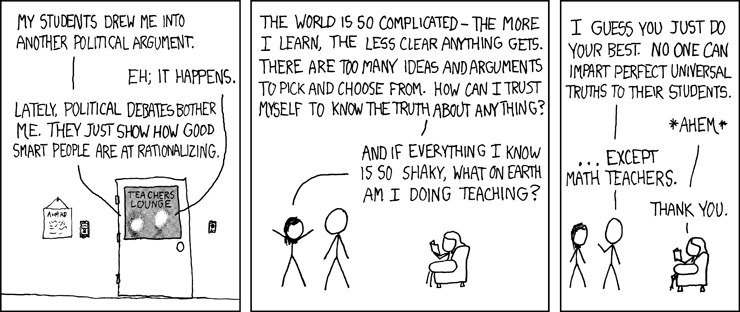
\includegraphics[width=\textwidth]{bilder/certainty.jpg}
\end{figure*}

\subsection{Die ersten Semester}

In der Mathematik startet man mit den Grundvorlesungen \vl{Analysis 1} und \vl{2} und \vl{Lineare Algebra 1} und \vl{2}; jede dieser vier Vorlesungen gibt jeweils 8~\gls{LP}. Die Vorlesungen \gls{Ana}~1 und \gls{LA}~1 finden im Wintersemester, \gls{Ana}~2 und \gls{LA}~2 finden im Sommersemester statt. 

Je nach der Wahl des zweiten Fachs können die ersten beiden Semester damit sehr voll sein. Viele Lehramtsstudierende konzentrieren sich deshalb entweder auf Mathematik und hören nur wenige Vorlesungen aus dem zweiten Fach oder entscheiden sich für eines der beiden Module, also entweder den \vl{Analysis} oder \vl{Lineare Algebra}-Zyklus. Wichtig ist allerdings, dass \gls{LA}~1 die Orientierungsprüfung ist, die ihr bis zum Ende des dritten Semester bestanden haben müsst, sonst dürft ihr nicht weiter studieren.

Solltet ihr aber feststellen, dass euch vier Vorlesungen im ersten Semester zu viel sind, dann ist das kein Weltuntergang. Ihr solltet euch dann entweder ganz auf Mathematik oder nur auf eines der beiden Module \vl{Lineare Algebra} oder \vl{Analysis} konzentrieren. Das kann natürlich dazu führen, dass sich euer Studium um ein oder zwei Semester verlängert. Auch in anderen Bachelor-Studiengängen, zum Beispiel im Mathematik Bachelor 100\%, ist die durchschnittliche Studienzeit höher als die Regelstudienzeit. Wenn ihr länger als die Regelstudienzeit studiert, kann es sein, dass ihr für die zusätzlichen Semester kein BAföG mehr bekommt. Aber auch da gibt es Ausnahmen. Ihr solltet euch, falls ihr Vorlesungen in spätere Semester schiebt, frühzeitig bei den zuständigen Stellen informieren.

\subsection{Wahlpflichtbereich und Seminare}

Nachdem ihr die Grundvorlesungen absolviert habt, könnt ihr euch aussuchen, in welcher Reihenfolge ihr die Vorlesungen aus dem Wahlpflichtbereich hören wollt. Das sind
\begin{itemize}
  \item \vl{Algebra 1}
  \item \vl{Funktionentheorie 1} (\gls{FunkTheo})
  \item \vl{Einführung in die Wahrscheinlichkeitstheorie und Statistik} (\gls{WTheo0})
  \item \vl{Einführung in die Numerik} (\gls{Num0})
\end{itemize}
alle wieder jeweils zu 8~\gls{LP}. 

Im Bachelor müsst ihr mindestens drei der vier zur Wahl stehenden Vorlesungen hören. Dabei müsst ihr beachten, dass ihr am Ende des Master of Education alle vier Wahlpflicht-Vorlesungen bestanden haben müsst. Das heißt, ihr könnt im Bachelor alle vier Wahlpflicht-Vorlesungen hören oder ihr besucht im Bachelor drei Wahlpflichtvorlesungen und eine Veranstaltung aus dem Angebot der Fakultät. Dann belegt ihr die euch noch fehlende Wahlpflicht-Vorlesung im Master. Bei eurer Wahl der Veranstaltung aus dem Angebot der Fakultät ist das Modulhandbuch zum 50\%-Bachelor zu beachten. Falls ihr euch ein Seminar auswählt, solltet ihr auf die Leistungspunkte achten. Da im Allgemeinen ein Seminar nur mit 6 \gls{LP} eingeht, kann es sein, dass die Dozentin beispielsweise eine schriftliche Ausarbeitung oder ähnliches als „Extra“-Leistung für die zusätzlichen 2 \gls{LP} fordert. Hier solltet ihr einfach die Dozentinnen frühzeitig ansprechen.

Außerdem müsst ihr im Bachelor noch jeweils ein \vl{Proseminar} und ein \vl{Seminar} machen; die bringen jeweils 6~\gls{LP}.

\subsection{Fachübergreifende Kompetenzen}

Als fachübergreifende Kompetenzen (FÜK) müsst ihr bildungswissenschaftliche Veranstaltungen belegen, da diese Zulassungsvoraussetzung für den Master of Education sind. Welche genau das sind, findet ihr im Artikel über das allgemeine Lehramt. Damit bleiben euch keine Leistungspunkte im Bereich der FÜK mehr übrig. Beachtet, dass pro Fach bis zu 2 \gls{LP} der insgesamt 20 FÜK-\gls{LP} bereits in den Pflichtvorlesungen euer beiden Studienfächer integriert sind. In \vl{Proseminar} und \vl{Seminar} im Mathematikanteil sind bereits 2 \gls{LP} für Fachdidaktik integriert. Diese zählen sozusagen bildungswissenschaftlich.

\subsection{Bachelor-Arbeit}

Als letztes bleibt noch die Entscheidung zu fällen, in welchem Fach ihr eure Bachelor-Arbeit schreiben wollt. Diese Entscheidung bestimmt, welches euer erstes Hauptfach ist und ob ihr dann mit einem Bachelor of Science oder einen Bachelor of Arts abschließt. In der Mathematik ist es per se leider nur mit bestimmten Fachkombinationen möglich, überhaupt eine Bachelorarbeit in Mathe zu schreiben. Für andere Kombinationen müsst ihr bei der Fakultät einen Antrag stellen, eine Ausnahme sollte aber bei entsprechender Motivation gut machbar sein.

Solltet ihr nach dem Doppelbachelor doch einen Fach-Master machen wollen, ist in den meisten Fächern dann auch die Bachelorarbeit in diesem Fach Zulassungsvoraussetzung für den Fach-Master.
%\newpage\Large\mathphyssubsubsec{Lehramt Physik}\small
\section{50\%-Bachelor Physik (Lehramt)} % oder: physik-Lehramt?

Der 50\%-Bachelorstudiengang Physik ersetzt ab dem Wintersemester 15/16 den Physik-Lehramtsstudiengang. Er hat einerseits die Aufgabe, die notwendigen fachlichen Kompetenzen für den Physikunterricht beizubringen und den Übergang zum Master of Education zu ermöglichen. Andererseits soll ein Übergang in den Physik-Masterstudiengang möglich sein. Es ist unausweichlich, dass der so entstehende Studiengang für keinen der beiden Wege die optimale Lösung darstellt. Dennoch versucht der Studiengang, diese Bedingungen irgendwie umzusetzen. Wie, wird im Folgenden vor diesem Hintergrund beschrieben.

\subsection{Fächerkombinationen}

Gemäß Prüfungsordnung darf der 50\%-Bachelor Physik mit allen anderen 50\%-Studiengängen an der Universität Heidelberg, die für einen Master of Education qualifizieren, kombiniert werden. Eine explizite Liste findet sich in Anlage 8 der Prüfungsordnung für den Physik-Bachelor (gemeinsame Prüfungsordnung für 100\%- und 50\%-Bachelor). Unabhängig von der Fächerkombination darf am Ende dieses Studiums die Bachelorarbeit in Physik geschrieben werden. Allerdings ist die Kombination mit Mathematik zu empfehlen, da nur so die notwendigen mathematischen Grundlagen erworben werden können, siehe dazu Abschnitt „Mathematische Grundlagen“.

\subsection{Arbeitspensum}

Wie erwähnt muss der 50\%-Bachelor Physik für den Physik-Master qualifizieren. Dies heißt, dass die grundlegenden Vorlesungen „Experimentalphysik“ 1-5 (\gls{Ex}) und „Theoretische Physik“ 1-4 (\gls{Theo})\footnote{Die Abkürzung „Theo“ kann zu Verwirrungen mit Informatikern führen, da diese das als „Theoretische Informatik“ verstehen.} verpflichtend vorgeschrieben und in den ersten fünf, bzw. vier Semestern gehört werden müssen. Dies führt besonders in den ersten beiden Semestern zu einem hohen Arbeitspensum: Ist das zweite Fach beispielsweise Mathematik, so müssten im ersten Semester die Vorlesungen Ex 1, Theo 1, „Analysis 1“ (\gls{Ana}) und „Lineare Algebra 1“ (\gls{LA}) gehört werden. Zum Vergleich: Für den 100\%-Bachelor Physik sieht die Fakultät 3 Vorlesungen dieses Umfangs pro Semester als angemessen an.

Im alten Lehramtsstudiengang wurde daher die Empfehlung ausgesprochen, die Vorlesungen der Theoretischen Physik um ein Jahr nach hinten zu schieben -- Theo 4 war damals aber nicht verpflichtend, sodass dies nicht zur Überschreitung der Regelstudienzeit von 6 Semestern führte. Für Studierende, die nicht auf BAföG (das nach der Regelstudienzeit gewöhnlich nicht mehr gezahlt wird) angewiesen sind, kann es auch weiterhin eine Option sein, Vorlesungen aus den ersten beiden Semestern aufzuschieben. Zu beachten ist allerdings, dass die in der Vorlesung Theo 1 behandelten Mathematischen Methoden in den Experimentalphysikvorlesungen verwendet werden. Zudem beträgt die Höchststudiendauer 9 Semester, nach denen man (außer nach Härtefallantrag) automatisch exmatrikuliert wird.

Die Semester 3-6 sind vom Arbeitsaufwand etwas geringer und außerdem hat man sich da dann schon an das Lernen an der Universität gewöhnt. Dabei ist stets der Großteil der Arbeit auf die Vorlesungszeit konzentriert, während in der vorlesungsfreien Zeit (abgesehen von Praktika) nicht viel geschieht.

Ziel dieses Abschnittes ist es sicherlich nicht, euch zu verunsichern oder gar Angst zu machen. Es ist durchaus problemlos möglich, die Vorlesungen wie vorgesehen zu absolvieren und mit guten Noten zu bestehen. Dies erfordert aber über das Semester hinweg disziplinierte Arbeit an den Übungszetteln für alle vier Vorlesungen. Die Erfahrung zeigt, dass es Studierende gibt, die mit diesem Arbeitspensum überlastet sind und dazu übergehen Übungsaufgaben abzuschreiben und so ins Hintertreffen geraten. Für ebenjene sei die Option aufgezeigt, dass es möglich ist, beispielsweise die Vorlesung Ana 1, oder möglicherweise Theo 1 um ein Jahr zu verschieben um so in der Lage zu sein, sich auf die verbleibenden drei Vorlesungen zu konzentrieren. Wir als Fachschaft, wie auch andere Anlaufstellen, stehen gerne als Ansprechpartner bereit, um bei derartigen Fragestellungen von unseren Erfahrungen zu berichten und Ratschläge zu geben.

\subsection{Mathematische Grundlagen}

„Mathematik ist die Sprache der Physik“ -- heißt es so schön und ist in der Tat korrekt. Man könnte sogar weiter gehen und sagen, dass die Menschheit nur deshalb begonnen hat, Mathematik zu betreiben, weil sich damit die Natur beschreiben lässt. Dies heißt aber auch, dass alle, die Physik betreiben -- sei es an Schulen, Universitäten oder in der Wirtschaft -- ein Grundverständnis für Mathematik benötigen. Für diejenigen unter euch, die Mathematik als zweites Fach gewählt haben, ist das Folgende nicht relevant, da die dort vorgesehenen Mathematik-Vorlesungen sicher mehr als nur ein Grundverständnis für Mathematik beibringen. Für alle anderen ist es aber vor gewisser Wichtigkeit.

Vieles der Mathematik, die in den ersten Semestern gebraucht wird, wird in den Physik-Vorlesungen behandelt. Grund dafür ist, dass die Fakultät für Mathematik und Informatik die Inhalte ihrer Vorlesungen natürlich an ihren eigenen Zielen und nicht denen des Physik-Studienganges ausrichtet. So beinhaltet beispielsweise die Vorlesung Theo 1 einen großen Mathematik-Teil, in dem beispielsweise die Lösung von Differentialgleichungen behandelt wird.

Allerdings sind nicht ohne Grund für den 100\%-Bachelorstudiengang Physik die Vorlesungen LA 1 sowie wahlweise „Höhere Mathematik für Physiker“ 2 und 3 (\gls{HoMa}) oder Ana 2 und 3 vorgeschrieben. Wichtige mathematische Konzepte wie Fouriertransformation werden in HöMa und Ex zeitgleich behandelt und die theoretische Beschreibung der Quantenmechanik ist ohne Kenntnis über Eigenvektoren aus LA 1 nicht zu verstehen. Das Beste wäre also, wenn all jene, die nicht Mathematik als zweites Fach gewählt haben, zumindest LA 1 vor Theo 4 hören (oder ein Buch lesen) würden. Besser sogar LA 1 und HöMa 2 und 3 oder Ana 2 und 3. Diese Vorlesungen sind im Modellstudienplan allerdings nicht vorgesehen, wodurch dies quasi freiwillige Zusatzarbeit wäre. Wie schon erwähnt könnte man auch hier in Erwägung ziehen, gewisse Vorlesungen aufzuschieben, um die notwendigen Mathematikkenntnisse vorher zu erlangen.


\subsection{Interdisziplinäres Modul}

Um denjenigen, die das Ziel haben, mit einem Fachmaster nach dem 50\%-Bachelorstudiengang fortzufahren, die Pflicht zu nehmen, Module in den Bildungswissenschaften zu absolvieren, sieht der 50\%-Bachelor Physik vor, dass man die Entscheidung zwischen Fachmaster und Master of Education schon im 5. Semester trifft. In 5.\,\&\,6. Semester kann man nämlich zwischen besagten Modulen in den Bildungswissenschaften auf der einen Seite (Lehramtsoption) und Praktika und Seminar auf der anderen Seite (interdisziplinäre Option) wählen. Ersteres ist notwendig für die Zulassung zum Master of Education, zweites zielt auf einen Fach-Master ab. Genauer ist dies in Anlage 9 Der Prüfungsordnung beschrieben.


\subsection{Zulassung zum Master Physik}

Dies Zulassungsordnung des Masterstudiengang Physik ist sehr freundlich gegenüber Studierenden. Es wird als Voraussetzung lediglich ein Anteil von 50\% Physik-relevanter Inhalte im Bachelorstudium gefordert. Dies ist gewährleistet, wenn man die Bachelorarbeit in Physik schreibt und die zuvor beschriebene interdisziplinäre Option wählt. Einer Zulassung zum Physik-Master steht damit nichts im Wege.

\subsection{Prüfungsordnung}

Die Prüfungsordnung (PO) ist wie das Modulhandbuch ein Dokument, welches ihr prinzipiell alle zumindest einmal lesen solltet. Darin ist festgelegt, wie das Studium grundsätzlich abzulaufen hat, von Prüfungsmodalitäten, über Punktevergabe etc. Zu finden ist die PO auf der Universitätsseite, unter der Kategorie 'Im Studium' bzw. einfach unter dem Link\footnote{\url{https://www.uni-heidelberg.de/md/studium/download/a14-01-1-10.pdf}}.

% !TEX ROOT = ../ersti.tex
\section{Beratung und Informationen zum Lehramt}
\label{lehramtkontakte}
%\newpage\subsection{\Large Beratung und Informationen zum Lehramt}%FIXME

Zum Studium mit Berufsziel Lehrerin in der gestuften Bachelor-Master-Struktur informieren die Heidelberg School of Education (HSE) mit ihren Informationsveranstaltungen und die Zentrale Studienberatung/Career Service (ZSB).
\begin{itemize}
\item \textbf{Service Portal für Studierende} \newline
    Seminarstraße 2, im Erdgeschoss (am Haupteingang links)
    Öffnungszeiten: Mo - Do 10 - 16 Uhr, Fr 10 - 14 Uhr; \newline
    Termin für ein Beratungsgespräch: Tel.: 0 62 21 / 54 - 54 54, E-Mail: studium@uni-heidelberg.de \newline
    Allgemeine Informationen\footnote{\url{https://www.uni-heidelberg.de/studium/interesse/abschluesse/lehramt.html}}

\item Wer sich für den Master of Education interessiert, kann sich hier über die fachspezifischen Zugangs- und Zulassungsvoraussetzungen informieren: \newline
    Teilstudiengang Mathematik\footnote{\url{https://www.uni-heidelberg.de/studium/interesse/abschluesse/mathematik_masterofeducation.html}} \newline
    Teilstudiengang Physik\footnote{\url{https://www.uni-heidelberg.de/studium/interesse/abschluesse/physik_masterofeducation.html}} \newline
    Teilstudiengang Informatik\footnote{\url{https://www.uni-heidelberg.de/studium/interesse/abschluesse/angewand_informatik_masterofeducation.html}}

\item Auskünfte zu den Staatsprüfungen gibt es beim \textbf{Landeslehrerprüfungsamt} (LLPA) Baden-Württemberg, Außenstelle Karlsruhe\footnote{\url{http://www.llpa-bw.de/,Lde/Startseite/Aussenstellen+des+LLPA/beim+Regierungspraesidium+Karlsruhe}} \newline
    Hausanschrift: Hebelstraße 2, 76133 Karlsruhe, Postanschrift: 76247 Karlsruhe \newline
    Frau Zimmer-Kraft (Leiterin): Tel. 0721/926-4500, hannelore.zimmer-kraft@rpk.bwl.de \newline
    Prüfungsberatung (Staatsexamen) findet \beratungpaedagogik, in der Zentralen Universitätsverwaltung (ZUV), Seminarstraße 2, 1. OG, Raum 161 statt.

\item Der AK Lehramt des StuRa \footnote{\url{http://www.stura.uni-heidelberg.de/arbeitskreise/ak-lehramt.html}}, dieser gibt auch den Newsletter "Lehrerzimmer" über aktuelle Entwicklungen beim Lehramt und die Arbeit des Arbeitskreis heraus, außerdem haben sie einen Hitchhikers-Guide für das Lehramtsstudium erarbeitet \footnote{\url{https://www.stura.uni-heidelberg.de/fileadmin/Dokumente/AKs/Lehramt/LehramtsGuideHeidelberg.pdf}, der Physik-Abschnitt ist jedoch nicht aktuell.}. Der AK freut sich immer über neue Mitstreiterinnen bei ihren regelmäßigen Treffen.  \newline AK Lehramt des StuRa, c/o~StuRa-Büro, Albert-Ueberle-Straße~3-5; Tel:~0\,62\,21/54\,24\,56

\item Die Mitglieder der Studienkommissionen sind insbesondere in Angelegenheiten im Zusammenhang mit den Modulhandbüchern und Prüfungsordnungen gute Ansprechpartnerinnen.

\item Bei allen Lehramtsfragen, bei denen ihr nicht wisst, an wen ihr sie stellen sollt, oder die sich aufs Lehramt beziehen und bisher niemand beantworten konnte, könnt ihr diese der Online Lehramtsberatung der HSE \footnote{\url{https://onlineberatunglehramt.hse-heidelberg.de/}} stellen. Sie beantworten euch alle Fragen zur Lehramtsoption im Bachelor, zur Zulassung zum Master und zum Master of Education. Hier erhaltet ihr eine schnelle Auskunft, an wen ihr euch bei Schwierigkeiten wenden könnt.


%\item Noch mehr Infos gibt es im Café mit Lehramtsberatung im Erziehungswissenschaftlichen Seminar, Do 14 bis 18 Uhr, anschließend von 18 bis 20 Uhr Vorträge, Filme und Infos für Lehramtsstudierende.
\end{itemize}


%~ \begin{figure}[h]
%~ \centering{
    %~ \includegraphics[width=3.5cm]{bilder/newton_1.png}
    %~ \hspace{0.55cm}
    %~ \includegraphics[width=3.5cm]{bilder/newton_2.png}
    %~ \hspace{0.55cm}
    %~ \includegraphics[width=3.5cm]{bilder/newton_3.png}
%~ }
%~ \end{figure}


%%%%%%%%%%%%%%%%%%%%%%%%%%%%%%%%%%%%%%%%%%%%%%%%%%%%%%%%%%%%%%%%%%%%%%%%%%%%
\chapter{Studieren -- wie geht das?}
\section{Lehrveranstaltungen an der Uni}
Im Gegensatz zur Schule gibt es an der Uni eine Reihe verschiedenartiger Veranstaltungen, in denen der Lehrstoff vermittelt werden soll. Im wesentlichen sind das: Vorlesungen, Übungen, Seminare und Praktika. Ihr habt im ersten Semester nur mit den ersten beiden zu tun. Diejenigen unter Euch, die Physik studieren, werden ab dem zweiten Semester auch Praktika machen. Proseminare werden in Mathe ab dem zweiten Semester angeboten. Beides braucht Euch also jetzt noch nicht zu beunruhigen.

Theoretisch sollte in den Vorlesungen eine Dozentin oder ein Dozent ein abgestecktes Teilgebiet der Mathematik bzw. Physik vermitteln.

Die Praxis sieht jedoch oft anders aus. In der Physik werden in atemberaubenden Tempo erstaunliche Phänomene vorgeführt und zur Erklärung noch erstaunlichere Formeln herangezogen, oft unterstützt durch erstaunlichste Versuche (die mitunter zur Multi-Media-Show geraten).

In Mathe bedecken die Profs in ebenfalls atemberaubendem Tempo gleichmäßig die Tafel mit ebenfalls erstaunlichen Zeichen die, kaum definiert, bereits in abenteuerliche Beweise verwickelt werden. Diese wiederum ermuntern dann einige unterforderte Studis dazu, Quervergleiche zum Lebesgueschen Lemma und ebenfalls verwirrenden Korollaren vorzuschlagen.

Es gibt zwei Wege, um trotz oft unbefriedigender Vorlesungspraxis an Lehrstoff zu kommen, d.h. etwas zu verstehen und nicht gleich am Anfang den Faden zu verlieren. Der eine ist, Fragen zu stellen, auch wenn das häufig Überwindung kostet. Es ist dabei gar nicht so wichtig, ob mit einer Frage etwas sofort klar wird, es ist schon gut, dass durch eine Frage den anderen und sich selbst Gelegenheit gegeben wird, die eigenen Gedanken zu ordnen (und nicht nur mitschreiben zu müssen). Außerdem wird nur so den DozentInnen gezeigt, dass es überhaupt Fragen gibt und nicht alles selbstverständlich ist. Dabei ist zu sagen, dass man sich mit Fragen nicht unbedingt eine Blöße gibt, denn manche scheinbar „blöde“ Frage hat schon viele DozentInnen aus dem Konzept geworfen.

Die andere Methode folgt dem Motto: „Gemeinsam macht stark“ . Wenn ihr Euch in Arbeitsgruppen zusammensetzt, könnt ihr Vieles klären, was Euch alleine völlig unerklärlich schien. Für das Lösen der Übungsaufgaben (siehe unten) ist es sowieso unerlässlich zusammenzuarbeiten, denn nur so könnt ihr damit klar kommen.

Mit dem Wort „Übungen“ wird eigentlich zweierlei bezeichnet: Einerseits die wöchentlich ausgegebenen Übungsaufgaben, die ihr für Eure Scheine braucht (siehe dort), andererseits die Übungsgruppen, in denen die Aufgaben besprochen und Probleme aus den Vorlesungen geklärt werden sollen. Auch hier gibt es wieder Unterschiede zwischen Mathe/Informatik und Physik: In Physik werden die Übungen in der Regel mindestens von Promovierten, oft auch von Habilitierten (also Profs) gehalten, die jedoch der Studiertätigkeit ziemlich entwachsen sind. Dementsprechend akademisch geht es häufig zu, viele halten eigene Privatvorlesungen. Und auch hier gilt es, so viele Fragen wie möglich zu stellen. Im ersten Semester werdet ihr neben dem fakultativen Basiskurs je zwei Semesterwochenstunden Übungen in Experimentalphysik und Theoretischer Physik haben. Manchmal werden vor Klausuren auch noch Sonderstunden angeboten, was ihr allerdings mit Eurem Tutor ausmachen müsst.

In Mathe und Informatik werden die Übungsgruppen von Studierenden höherer Semester, sogenannten Hiwis, gehalten. In den Übungsgruppen ist es am leichtesten, Probleme und Verständnisfragen zu klären. Leider werden aber oft nur die Aufgaben „heruntergerechnet“, man passt nicht mehr auf und versteht trotzdem nicht mehr von der Aufgabe als vorher. Sollte dies der Fall sein, fragt penetrant nach dem Sinn der Aufgabenstellung, nach ihrem Zusammenhang mit der Vorlesung oder was Euch sonst noch durch den Kopf geht. Nur so habt ihr eine Chance, dass ihr auch etwas aus der nervenzermürbenden Rechnerei lernt. Es kann z.B. ein Überblick gegeben werden, wozu man einen Satz später braucht oder auch mal ein Satz aus der Vorlesung ausführlich erklärt werden. Manchmal wird auch zum Beginn jeder Übung die letzte Vorlesung von einem der Teilnehmer zusammengefasst. Das gibt demjenigen die Gelegenheit, die Vorlesung intensiver nachzubereiten, und den anderen, nochmal eine einfachere Darstellung des Stoffes zu bekommen - und zwar von jemandem, der die gleichen Probleme wie man selbst hat und eine andere Sichtweise als die Profs.

Natürlich ist es auch möglich, alle Veranstaltungen (bis auf die Abgabe der scheinpflichtigen Übungsblätter) sausen zu lassen und nur aus Büchern zu lernen. Manchmal, bei sehr schlechten Vorlesungen, ist dies sogar die einzige sinnvolle Möglichkeit etwas zu lernen und seine Zeit sinnvoll zu nutzen. Hier muss jedeR seinen/ihren eigenen Stil entwickeln. Sprecht Euch aber in jedem Fall mit dem/der ÜbungsleiterIn ab, wenn ihr dort regelmäßig fehlen wollt, denn manchmal ist die Anwesenheit und das unfreiwillige Vorrechnen notwendige Voraussetzung für die Scheinvergabe.

\section{Vorlesungen}
\subsection{Einführung in die Praktische Informatik}
\label{info1}
Die Einführung in die Praktische Informatik (Info-I) ist für alle Informatik- und Mathe-Bachelors verpflichtend. Einstieg bilden einige Grundstrukturen und Abläufe in der Informatik, die im Verlauf dann angewendet werden müssen um gegebene Probleme zu lösen. Das passiert dann meist mit einem C++-Programm, wobei aber auch das Denken in informatischen Strukturen immer mitschwingt. Idealerweise hat man am Ende genug Herangehensweisen angehäuft um Aufgaben vor dem geisten Auge zu modellieren und später in richtigen Code umsetzen zu können. Vor allem MathematikerInnen sollten die Vorlesung nicht auf die leichte Schulter nehmen, auch wenn der geringe Aufwand dazu verleitet. Spätestens mit der „Numerik 0“ muss wieder programmiert werden -- sich darum drücken kann man also nicht. Auch für LehrämtlerInnen kann es interessant sein, die Vorlesung zu hören, um sich später den Einstieg in die Numerik zu vereinfachen.

\subsection{Analysis I}
\label{ana1}

Die Analysis I (Ana I) muss von den MathematikerInnen gehört werden, jedoch sind auch PhysikerInnen und InformatikerInnen nicht unbedingt schlecht beraten. Hier lernt ihr richtige, fundierte Mathematik in all ihrer Schönheit und Abstraktion (was sehr abstrakt sein kann). Diese Vorlesung hat mit dem Matheunterricht aus der Schule ähnlich viel gemeinsam wie mit dem Sportunterricht.

Ihr lernt das formell richtige Argumentieren und Beweisen und erhaltet einen Einblick darin, was das Gebäude der Mathematik eigentlich ausmacht und wie dieses aufgebaut ist. Inhaltlich beginnt sie mit der Konstruktion der reellen Zahlen, führt über Folgen und Reihen zur Stetigkeit von (reellen) Funktionen und schließlich zur Differential- und Integralrechnung. Der Arbeitsaufwand für die Vorlesung schwankt (je nach Prof) zwischen lächerlich und immens, auch hier sind zehn oder mehr Stunden für einen Zettel nicht unbedingt Seltenheit (Es lohnt sich Zettelgruppen zu bilden und gemeinsam zu rechnen). Was das unglaublich frustrierende und hilflose Gefühl betrifft, man würde nichts verstehen und wäre völlig falsch in seinem Studiengang, keine Angst, das haben alle. Wenig härtet so gut gegen Frust ab wie eine erbarmungslose Mathevorlesung im ersten Semester. Aber lasst Euch davon nicht täuschen, dass Begriffe, die ihr meint aus der Schule zu kennen, unnötig umständlich eingeführt werden. Es hat alles durchaus seine mathematische Berechtigung und schafft ein Fundament, auf das ihr später aufbauen werdet. Sich ein sauberes, formelles Vorgehen und Denken anzugewöhnen ist unabdingbar.

\subsection{Lineare Algebra I}
\label{la1}
Die Lineare Algebra I (LA I) hören MathematikerInnen, PhysikerInnen und (eventuell.) InformatikerInnen zusammen, bereitet Euch also auf eine sehr große Vorlesung vor. Neben den vielen Grundlagen die euch hier vermittelt werden,  handelt es sich inhaltlich um die Vektorrechnung, wie ihr sie bereits aus der Schule kennt. Diese wird jedoch viel allgemeiner und abstrakter als bisher eingeführt, was am Anfang etwas umständlich erscheint, später die Vorteile jedoch offenbar werden und „Sie sehen, dass das wieder eine Matrix wird und wir das selbe wie immer können“ (Prof. Wingberg). Im weiteren Verlauf kommen auf der Vektorrechnung aufbauend noch lineare Operatoren und Innenprodukträume hinzu, die euch Begriffe und Sätze wie Determinanten, Eigenwerte oder den Spektralsatz näher bringen. Die Inhalte werden euch euer ganzes Studium nicht mehr verlassen, da praktisch alle höheren Vorlesungen auf das mächtige Werkzeug der Linearen Algebra zurückgreifen.

\subsection{Höhere Mathematik für Physiker}
\label{mathephysik}

Die Mathematikausbildung für Physikerinnen sieht vor, dass ihr die Lineare Algebra 1 (\gls{LA}) im ersten Semester hört. Laut Modulhandbuch könnt ihr euch dann vor dem zweiten Semester entscheiden, ob ihr mit Analysis 2 und 3 (\gls{Ana}, was auch die Mathematikerinnen hören) oder mit Höhere Mathematik für Physiker (\gls{HoMa}) 2 und 3 weitermacht.

\subsubsection{Was spricht für HöMa?}
Die Vorlesung ist extra auf euch als Physikerinnen zugeschnitten und legt ihren Schwerpunkt auf die Vorlesungen Ana 1-3 in strafferer Form. Während Mathematikvorlesungen einer gewissen Freiheit unterliegen und es durchaus vorkommen kann, dass die Dozentin einen Schwerpunkt auf ihr Forschungsgebiet legt, hört ihr in HöMa größtenteils nur jene Dinge, die in der Physik auch verwendet werden. Außerdem kommen Beispiele gerne aus der Physik und liegen euch deshalb vielleicht näher. Trotzdem handelt es sich nicht um eine Schmalspurversion, sondern um eine vollwertige Mathematikvorlesung, die auch für zukünftige Theoretikerinnen nicht ungeeignet ist.

\subsubsection{Was spricht für die Analysis (Ana)?}
Die Analysis bietet als eine für Mathematikerinnen konzipierte Veranstaltung eine präzisere Formulierung der Definitionen, Sätze und insbesondere Beweise. Somit wird es möglich die mathematischen Hintergründe in der Physik besser zu durchdringen und weitergehende Verbindungen der Gebiete zu erkennen. Dieses tiefere Verständnis kann unter anderem in der theoretischen Physik oder auch in weiterführenden Matheveranstaltungen von Vorteil sein und lässt euch insgesamt mehr Freiheiten im weiteren Studienverlauf, besonders bezüglich der Mathematik. Zudem ist je nach Dozentin und Forschungsbereich auch eine gewisse Schwerpunktlegung (vor allem in der Ana 3) möglich.\\

Auf den ersten Blick mag es verwundern, dass ihr in die Ana 2 einsteigen sollt, ohne die erste Vorlesung dazu gehört zu haben. Dies ist theoretisch zumindest möglich, jedoch vermutlich mit ein wenig Mehraufwand verbunden. Trotzdem können mathematisch Ambitionierte natürlich auch die Ana 1 im ersten Semester hören, da diese eine schöne Einführung in den Themenbereich Analysis und die damit verbundenen Methoden darstellt. Das kann euch vor allem in weiterführenden Vorlesungen weiterhelfen; auch wird es eine große Erleichterung für die Ana 2 sein, wenn ihr schon ein wenig mehr mit der Materie und der Dozentin vertraut seit. Andererseits werdet ihr mit dem Kursprogramm auch so schon stark ausgelastet sein. Wenn ihr es mit vier Vorlesungen versuchen wollt, solltet ihr euch nach zwei bis drei Wochen entschieden haben, ob ihr das im ersten Semester durchhaltet oder nicht, da es für den Übungsbetrieb ziemlich blöd ist, wenn in der Mitte des Semesters viele Leute aussteigen.

% !TEX ROOT = ../ersti.tex
\subsection{Experimentalphysik 1: \\Mechanik und Wärmelehre}
\label{ex1}
Die Experimentalphysik 1 (\gls{Ex}) ist eigentlich eine sehr angenehme Vorlesung, um ins erste Semester zu starten, zumindest sofern ihr in der Schule irgendwann mal Physik hattet. Echte Verständnishürden stellen sich gerade im Mechanikteil im Allgemeinen nicht. Im Großen und Ganzen stellt sie einen Schnelldurchlauf durch die Entwicklung der Mechanik dar, von den Anfängen (diese liegen, je nach Prof, zwischen den alten Griechen und Newtons Axiomen) bis zu etwas ausgefeilteren Sachen, die sich aber alle noch im Rahmen des Schulstoffs bewegen sollten. Was diese Vorlesung dennoch von der Schule unterscheidet ist die \emph{Art} der Präsentation, größtenteils frontaler Vortrag, gespickt mit vielen Experimenten (Manchmal durchaus eine Art „Knoff-Hoff-Show“) und sehr viel schneller und mathematischer als ihr das von eurer Lehrerin gewohnt seit. Trotzdem ist dies die Vorlesung mit dem wahrscheinlich größten Unterhaltungswert eurer ganzen Universitätskarriere.

\begin{figure*}[b]
    \centering
    \begin{subfigure}[b]{.18\textwidth}
    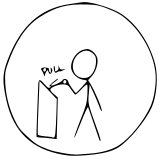
\includegraphics[width=\linewidth]{bilder/the_difference_1.png}	    
    \end{subfigure}
    \begin{subfigure}[b]{.18\textwidth}
    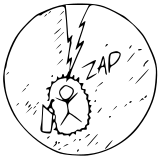
\includegraphics[width=\linewidth]{bilder/the_difference_2.png}
    \end{subfigure}
    \begin{subfigure}[b]{.18\textwidth}
    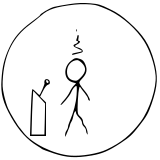
\includegraphics[width=\linewidth]{bilder/the_difference_3.png}
    \end{subfigure}
    \begin{subfigure}[b]{.18\textwidth}
    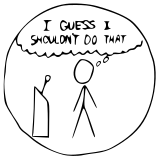
\includegraphics[width=\linewidth]{bilder/the_difference_4A.png}
    \end{subfigure}
    \begin{subfigure}[b]{.18\textwidth}
    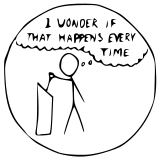
\includegraphics[width=\linewidth]{bilder/the_difference_4B.png}
    \end{subfigure}
\end{figure*}


\subsection{Theoretische Physik I - Mechanik und Mathem. Methoden}
\label{theo1}

Die Theoretische Physik I (Theo-I) beschäftigt sich mit der Newton'schen Mechanik und nützlichem mathematischen Werkzeug.

Hier werdet ihr im ersten Semester einige Zusammenhänge und Techniken einfach „vorgesetzt“ bekommen ohne sie völlig zu verstehen. Der genaue Grund, warum man das, was man da tut, eigentlich darf, wird im Normalfall erst in einer der späteren Mathevorlesungen klar, daran sollte man nicht verzweifeln. Dieses Vorgehen ist in der Physik nicht ungewöhnlich, was einer der Angriffspunkte von Witzen der Mathematiker über Physiker ist\dots

Ihr erhaltet hier aber nicht nur die mathematischen Techniken, die ihr in Eurem Studium brauchen werdet (und von denen ihr in vielen Fällen noch nie was gehört habt), sondern Euch wird auch eine theoretische Beschreibung der Mechanik vorgestellt. Diese unterscheidet sich im ersten Semester, bis auf einige seltsame Symbole und unglaubliche Umständlichkeit noch nicht sehr von der in der Ex-I, ab dem zweiten Semester tun sich zwischen den Sichtweisen jedoch Abgründe auf und ihr werdet verstehen, warum man auf diese Umständlichkeit bestanden hat.

Der Anspruch dieser Vorlesung an Verständnis und Wissen ist deutlich größer als in der Ex-I, womit ihr auch einen erheblich höheren Aufwand für die Bewältigung der Arbeitszettel einplanen könnt, je nach eigenem Interesse, Wissen und Perfektionismus sind zehn Stunden durchaus eine realistische Einschätzung für einen Zettel. Die Übungsgruppenleiter sind hier vor allem ältere Studierende, was den Vorteil hat, dass diese sich noch an ihre eigenen Probleme in ihrer Theo-I erinnern können und Euch das ganze verständlicher erklären können als der Theo-Prof es kann.

\phantom{mathphyssecnobar}
\newpage

\newpage


\begin{figure*}[t]
    \centering
    \begin{subfigure}[b]{.18\textwidth}
    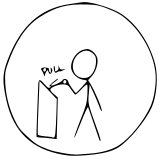
\includegraphics[width=\linewidth]{bilder/the_difference_1.png}	    
    \end{subfigure}
    \begin{subfigure}[b]{.18\textwidth}
    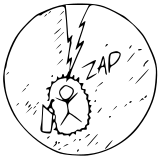
\includegraphics[width=\linewidth]{bilder/the_difference_2.png}
    \end{subfigure}
    \begin{subfigure}[b]{.18\textwidth}
    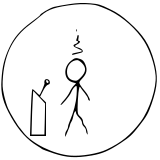
\includegraphics[width=\linewidth]{bilder/the_difference_3.png}
    \end{subfigure}
    \begin{subfigure}[b]{.18\textwidth}
    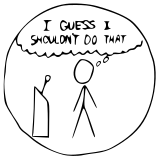
\includegraphics[width=\linewidth]{bilder/the_difference_4A.png}
    \end{subfigure}
    \begin{subfigure}[b]{.18\textwidth}
    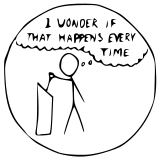
\includegraphics[width=\linewidth]{bilder/the_difference_4B.png}
    \end{subfigure}
\end{figure*}

\section{Durchgefallen -- Was tun?}

In eurem Studium wird es aller Voraussicht nach hin und wieder vorkommen, dass ihr durch die eine oder andere Klausur durchfallt. Das ist an und für sich auch kein großes Problem. Zuerst einmal ist es aber wichtig, zu wissen, was es eigentlich heißt, „durchgefallen“ zu sein.

Die meisten Leute setzen „durchgefallen“ mit „die Klausur nicht bestanden haben“ gleich. Das ist nicht ganz falsch, aber auch nicht ganz richtig. Ihr müsst nämlich zwischen Klausur und Prüfungsleistung\footnote{ Der Unterschied zwischen Prüfungsleistung und Prüfungsversuch besteht primär sprachlich, beide bezeichnen meistens Klausur und Nachklausur als Einheit.} unterscheiden. In fast allen Grundvorlesungen werden eine Klausur und eine Nachklausur geschrieben, die zusammen als ein Prüfungsversuch zählen. Erst wenn ihr Klausur \emph{und} Nachklausur nicht bestanden habt, habt ihr die entsprechende Prüfungsleistung nicht bestanden. Ihr habt dann die Möglichkeit, die Prüfungsleistung zu wiederholen. Dazu hört ihr das Modul dann einfach nochmal, und habt dann ein weiteres Mal Klausur und Nachklausur vor euch. Besteht ihr beide nicht, könnt ihr einen Härtefallantrag stellen, und versuchen, vor dem Prüfungsausschuss zu begründen, warum ihr vier Klausuren nicht bestanden habt. In der Physik habt ihr zusätzlich in zwei Modulen einen dritten Prüfungsversuch.\footnote{Das nennt sich dann in der Physik „Jokerregelung“} Wie genau das geregelt ist, steht an entsprechender Stelle im Modulhandbuch. In der Informatik habt ihr die Chance in zusätzlich vier Modulen einen dritten Prüfungsversuch durchzuführen.

\subsection{Orientierungsprüfung}
Eine Ausnahme von dieser Regelung stellt die sogenannte Orientierungsprüfung dar. Diese Prüfung soll feststellen, ob ihr überhaupt geeignet seid, das Fach, das ihr studiert, zu studieren. Diese Prüfung müsst ihr, im Gegensatz zu allen anderen Prüfungen, bis spätestens zum Ende des dritten Semesters erbracht haben, und die Jokerregelung gilt hier nicht.

\subsection{Muss ich nochmal Zettel rechnen?}
Das kommt auf die Dozentin deiner Veranstaltung an. Es gibt einige, die finden, dass man die Zettel nicht nochmal rechnen muss, einige wollen, dass du die Zulassung noch mal neu erwirbst. So oder so ist es unglaublich hilfreich, die Zettel trotzdem noch mal zu rechnen. Zwei mal die gleiche Veranstaltung bei zwei verschiedenen Professorinnen ist eben doch ein Unterschied, und dass du Nachholbedarf hast, hast du ja schon gezeigt ;)

%\section{Was sind diese „Übungsgruppen“?}
\newpage\mathphyssecnobar{Was sind diese „Übungsgruppen“?}

%\subsection{Übungszettel}
\noindent In den meisten Vorlesungen müsst ihr, um zur Klausur zugelassen zu werden, Übungszettel rechnen. Das bedeutet, jede Woche werden irgendwo\footnote{Wo, wird in der ersten Vorlesung bekannt gegeben} Übungsaufgaben hochgeladen, die ihr euch ausdrucken und dann rechnen sollt. Weil das erfahrungsgemäß nicht so einfach ist, und meistens viele viele Fragen auftreten, gibt es Übungsgruppen.

\subsection{Übungsgruppen}
In fast allen Vorlesungen werden vorlesungsbegleitend sogenannte „Übungsgruppen“ angeboten. Diese Übungsgruppen sind dazu da, euch bei euren Problemen mit der Vorlesung zu helfen und die Zettel nachzubesprechen. Dazu seid Ihr natürlich nicht auf euch allein gestellt, sondern euch wird einE TutorIn zur Seite gestellt, die Euch bei allen Fragen, die auftreten, kompetente Hilfe bietet. Hier unterscheiden sich die Mathe/Informatik und die Physik: In der Physik werden die Übungsgruppen meistens mindestens von Masterstudenten, häufig auch von Doktoranden oder gar Profs gehalten. Dementsprechend studierendenfern sind diese oftmals, aber natürlich gibt es auch Tutoren, die geradezu geniale Übungsgruppen halten. Grundsätzlich gilt es aber, so viele Fragen wie möglich zu stellen, auch um dem Tutor Feedback zu eurem Kenntnisstand zu geben. In der Mathe werden die Übungsgruppen in den meisten Fällen von Studierenden höherer Semester gehalten, es ist durchaus nicht unüblich, einen Tutor zu haben, der die Vorlesung selber erst vor zwei Semestern gehört hat.

\subsection{Was bringt mir das?}
Die Übungszettel und die dazugehörigen Übungsgruppen sind erfahrungsgemäß der Ort, an dem euch der Stoff der Vorlesung nahe gebracht wird und ihr anfangt zu verstehen, was eigentlich in der Vorlesung vor sich geht. Eigentlich ist die Übungsgruppe also dazu da, die Vorlesung mit euch nachzuarbeiten, an den Stellen, an denen nicht klar ist was passiert, Hilfe zu bieten, mit euch die Zettel zu besprechen und einfach nochmal eine andere Darstellung zu liefern. Leider kommt es viel zu oft vor, dass in der Übung nur die Aufgaben „runtergerechnet“ werden, man irgendwann nicht mehr aufpasst und am Ende auch nicht mehr weiß, als vorher. Wenn das passiert, fragt penetrant nach dem Sinn der Aufgabenstellung, nach dem Zusammenhang mit der Vorlesung oder nach was euch sonst noch so durch den Kopf geht. Das ist eure einzige Chance, noch etwas aus der Rechnerei zu lernen.

\subsection{Anmeldung}
Ganz häufig stellen sich anfangende Studierende die Frage, ob sie sich zu den Übungen anmelden müssen. Die Antwort ist meistens „ja“. In der Physik nutzt man dazu das physikinterne Übungsgruppensystem\footnote{\url{https://uebungen.physik.uni-heidelberg.de/uebungen/}} Das System ist leider nicht besonders leistungsfähig. Da kann es schon mal vorkommen, dass es zu Zeiten, in denen die Übungsgruppenanmeldung großer Vorlesungen freigeschaltet werden, abkackt. Das ist aber auch kein Drama, und insbesondere kein Grund, das Rektorat zu alarmieren\footnote{Wann das wohl passiert ist…}, denn nach einigen Minuten hat sich das System dann auch wieder gefangen. Die Mathe geht wie immer ihren eigenen Weg, und hat mit dem Müsli\footnote{Mathematisches Übungsgruppen- und ScheinListenInterface:\\ \url{https://www.mathi.uni-heidelberg.de/muesli/}} ihr eigenes System. Das ist deutlich leistungsfähiger, deutlich besser und viel schöner, aber man kann als Physiker ja nicht alles haben. Die Informatik wiederum nutzt in 90\% aller Fälle das Moodle\footnote{\url{https://elearning2.uni-heidelberg.de/}}, das E-Learning-System der Uni Heidelberg. 90\% aller Nutzer sind sich einig, dass dieses System ganz doll Grütze ist, aber davon hat sich die Informatik noch nie beeinflussen lassen.

\section{Praktika}

In der Physik werdet ihr früher oder später Praktika absolvieren. Dabei geht es darum, dass ihr eure ganzen erworbenen Kenntnisse aus den Ex-Vorlesungen endlich anwendet, um eigene „Forschung“ zu betreiben.

\subsection{Wann ist das?}
In den Semesterferien zwischen dem zweiten und dem dritten Semester geht der Praktikums-Spaß mit dem AP 1\footnote{AP == AnfängerPraktikum} los. In eurem dritten Semester, den Semesterferien zwischen drittem und viertem Semester und im vierten Semester absolviert ihr die beiden Teile des AP 2. Ihr könnt euch dabei selber einteilen, welchen Teil ihr wann macht. Erfahrungsgemäß ist AP 2.1 etwas mehr und etwas komplizierter, daher ist es empfehlenswert, diesen Teil in den Semesterferien zu machen.

Sobald ihr eure Anfängerpraktika hinter euch habt, dürft ihr mit dem FP \footnote{FP == FortgeschrittenenPraktikum} anfangen. Auch hier gibt es wieder zwei Teile und ihr müsst aus beiden Teilen mindestens 3 Versuche machen, insgesamt stehen 8 Versuche auf dem Plan. Zu einem davon müsst ihr dann auch noch einen Vortrag halten, und zu einem müsst ihr eine ganz besonders ausführliche Auswertung schreiben. Das FP wird aber nicht mehr -- wie die AP -- als Blockveranstaltung angeboten, sondern ihr dürft euch eure Versuche selber so legen, wie es euch gerade passt -- vorrausgesetzt der Versuch wird dann, wann ihr wollt, angeboten.

\subsection{Und wie geht das?}
Das grundlegende Konzept der Praktika ist, dass ihr selber einige Ergebnisse aus Ex 1-5 reproduziert. Sei es jetzt die Erdbeschleunigung über Pendelschwingungen oder die Boltzmannkonstante aus Brown'scher Bewegung, ihr messt selber, wertet eure Ergebnisse selber aus und müsst selbst bewerten, ob das, was ihr gemacht habt, signifikant ist.

Dabei gehen fast alle Versuche nach dem gleichen Schema vor: Ihr bekommt ein Skript, in dem die Theorie des Versuchs, die Durchführung und die Auswertung ausführlich beschrieben sind. Ihr schreibt dann mithilfe dieses Skripts eine Einleitung zu eurem Versuch, in der ihr in eigenen Worten formuliert, was ihr eigentlich tun werdet. Am Tag des Versuchs selber werdet ihr von eurem Betreuer dann abgefragt, ob ihr Bescheid wisst, was zu tun ist. Danach messt ihr alle wichtigen Größen für diesen Versuch selber an den entsprechenden Apparaturen. Ist das geschehen, schreibt ihr eine Auswertung, in der ihr die gemessenen Größen auswertet und das eigentliche Resultat produziert.

\section{Seminare}

In eurem Studium werdet ihr früher oder später über Seminare und Proseminare stolpern, in der Mathe und Info früher und mehr als in der Physik. Seminare dienen dazu, dass ihr euch selbst ein Thema erarbeitet und dann lernt, dieses vorzustellen.

Seminare fangen immer mit der Seminarvorbesprechung an. Alle Studentinnen, die an dem Thema des Seminars interessiert sind, treffen sich dort. Es werden die verschiedenen Vortragsthemen von der Seminarbetreuerin vorgestellt. Im Anschluss werden diese an die verschiedenen Teilnehmerinnen verteilt.

Sobald ihr also euer Thema habt, habt ihr (je nach Thema) zwei Wochen bis ein Semester Zeit, um euch vorzubereiten. Ihr lest also das entsprechende Kapitel in dem Buch oder dem Paper, nach dem das Seminar gehalten wird, oder beschäftigt euch sonst mit dem Thema. Im Unterschied zu Vorlesungen arbeitet ihr euch selber in das Thema ein, müsst euch Zusammenhänge selber überlegen und seid dann selbst gefordert, denn ihr müsst das zuvor Gelernte selber an die Tafel und in einen Votrag bringen.

Falls ihr irgendwo in eurer Vorbereitung über Dinge stolpert, die ihr nicht versteht, oder falls irgendwo Fragen auftauchen, die ihr selber nicht beantwortet bekommt, könnt ihr euren Seminarbetreuerin fragen, denn genau das ist ihr Job.

\subsection{Wie komme ich an ein Seminar?}

Die Suche beginnt für Physikerinnen in der Vorlesungsfreien Zeit, für Mathematikerinnen und Informatikerinnen bereits während dem alten Semester \-- zum Teil in der Klausurenphase. Die Seminarvorbesprechungen in der Physik finden in der ersten Woche des neuen Semesters statt. In der Mathe und Informatik liegen diese zum Teil auch in der letzten Woche des alten Semesters, daher müsst ihr euch rechtzeitig über das Seminarangebot des nächsten Semesters informieren.

Zunächst schaut ihr ins LSF. Dort stehen bis zum Anfang des Semesters alle angebotenen Seminare. Um früher Informationen über die Vorbesprechungen zu bekommen ist es in der Mathe und Info nötig zusätzlich an folgenden Orten zu suchen:

\begin{itemize}
	\item an Aushängen im Erdgeschoss des Mathematikons
	\item im Müsli
	\item auf Webseiten der Dozenten, die das gewünschte Fachgebiet abdecken.
\end{itemize}

Nachdem ihr wisst, wann diese stattfindet, geht ihr in die Vorbesprechung. Dort wählt ihr ein Thema aus und bekommt einen Termin für den Vortrag.

\subsection{Proseminar oder Seminar?}
Für viele Leute ist ein Seminar das erste Mal, dass sie an der Tafel stehen.  Weil in Seminaren der Inhalt doch stark im Vordergrund steht, gibt es in der Mathe und Informatik zusätzlich zu Seminaren auch noch sogenannte Proseminare. Der Unterschied ist der folgende: Seminare sind dazu da, euch ein bestimmtes Thema, das für eine Vorlesung zu speziell wäre und zu wenig Leute interessiert, nahe zu bringen. Diese Themen sind meistens relativ komplex und ihr müsst euch selber mit dem Inhalt beschäftigen, selber Gedanken machen und quasi selber „Mathe“ (oder ähnliches) produzieren. Der Fokus liegt also klar auf der Mathe bzw. Informatik und wenig auf eurem Vortrag. In Proseminaren hingegen sollte der Fokus auf dem Vortrag, und weniger auf dem Inhalt liegen. Der ist natürlich auch wichtig, und man sollte nicht erwarten, dass ein Proseminar inhaltlich einfach wird, aber meistens sind auch schwere Proseminare weniger anspruchsvoll als leichte Seminare. Nach eurem Vortrag wird dieser daher deutlich ausführlicher analysiert und nachbesprochen, als es bei einem Seminar der Fall wäre.

\subsection{Und wozu mache ich das?}
Für ein Seminar gibt es drei Gründe.

Der erste, und wohl offensichtlichste ist, dass es im Bachelor Pflicht ist.

Der zweite und wohl ebenso offensichtliche ist, dass Seminare die Möglichkeit bieten, Themengebiete kennen zu lernen, die in den Grundvorlesungen nicht vorkommen oder nur angeschnitten werden, oder sich in bestimmten Bereichen zu vertiefen.

Der dritte und nicht ganz so offensichtliche Grund ist, dass die meisten Profs Seminare nutzen um die Studentinnen kennenzulernen, die bei ihnen Bachelorarbeiten schreiben wollen. In der reinen Mathe geht das sogar so weit, dass es relativ unmöglich ist, eine Bachelorarbeit zu bekommen, ohne vorher ein Seminar gehört zu haben. Die angewandte Mathe sieht das nicht ganz so eng, aber auch da ist ein Seminar oder eine Vorlesung bei der entsprechenden Professorin empfehlenswert. In der Physik haben Seminare keinen so großen Stellenwert wie in der Mathe und Info, in den meisten Fällen hören Bachelorstudentinnen genau eines -- ihr Pflichtseminar. 

\section{Lehrbücher}

Bücher sind in erster Linie eine Geschmackssache. Die meisten Bücher, die hier aufgelistet werden, behandeln Elemente des Stoffes, der für die ersten zwei Semester gebraucht wird. Das richtige Buch für sich selbst zu finden, geht aber nur durch Ausprobieren! Jedem Lerntyp liegen unterschiedliche Herangehensweisen und damit auch unterschiedliche Bücher. Hier für sich selbst den richtigen Weg zu finden, kann durchaus seine Zeit dauern -- macht euch deshalb nicht verrückt wegen der Büchersuche, die Physik und Mathe ist letztendlich in allen Werken die Gleiche.

Es ist jedoch durchaus empfehlenswert, in einer ruhigen Minute mal ein Thema in verschiedenen Büchern nachzulesen. Dabei lernt man nicht nur viel über die eigene bevorzugte Herangehensweise, die unterschiedlichen Blickwinkel können auch dazu beitragen, ein Thema umfassender (oder überhaupt erst) zu verstehen.

Neben der Möglichkeit, sich in der Universitätsbibliothek Bücher auszuleihen, darf hier auch ein Hinweis auf den Lesesaal nicht fehlen: Im Erdgeschoss der UB befindet sich ein großer Bereich mit Arbeitsplätzen, in dem ein großer Teil der Lehrbücher als Ansichtsexemplare ausliegen. Dort kann man sich die verschiedenen Bücher in Ruhe genauer ansehen, außerdem wird dieser Bereich von manchen Studierenden auch als Lernumgebung sehr geschätzt, da dort absolute Ruhe und eine sehr konzentrierte Lernatmosphäre herrscht und man alle nötigen und unnötigen Nachschlagewerke direkt vor Ort hat. Ähnliches gilt übrigens auch für die Präsenzbibliotheken der Fakultäten (s.u.).

Falls ihr vorhabt, ein Buch zu kaufen, dann lasst Euch Zeit dafür und leiht euch die Bücher lieber erst einmal aus (alle hier vorgestellten Bücher sind im Bestand der Leihbibliothek). Beim ersten Durchblättern eines Buches kann man meistens nicht feststellen, ob einem die Art und Weise der Stoffvermittlung liegt. Das führt häufig im ersten Semester dazu, dass in Extremfällen kleine dreistellige Beträge für Fachliteratur ausgegeben werden, die anfangs als absolut notwendig erscheint und sich dann nach einiger Zeit doch als mehr oder weniger nutzlos erweist, weil einem die spezielle Herangehensweise des Buches zufällig nicht liegt\dots

Für viele Vorlesungen haben die Dozierenden ein Skript erstellt, was häufig eine gute Hilfe bei der Nachbereitung des Stoffes ist. Einige dieser Skripte werden auch gedruckt und im Laufe des Semesters in den Vorlesungen ausgeteilt. Anschließend sind sie im Fachschaftsraum kostenlos erhältlich -- kommt einfach bei uns vorbei und fragt nach, ob das auch bei euren Vorlesungen der Fall ist.

Weiterhin solltet ihr auf jeden Fall die Skriptensammlung\footnote{\url{http://mathphys.fsk.uni-heidelberg.de/w/hauptseite/skripte/}} der Fachschaft im Netz durchstöbern. Unter „Skriptensammlung (PDFs)“ findet ihr unsere Links zu Vorlesungsskripten (dort finden sich passende Skripte zu fast jeder Vorlesung).

\subsubsection{Analysis}
\begin{description}
\item[Forster]{
		Die ersten zwei Bände behandeln recht knapp und kompakt den Stoff der ersten zwei Semester des Analysis-Kurses. Der dritte Band ist ebenfalls knapp geschrieben, allerdings sehr umfangreich, so dass meist nicht einmal die Hälfte des Buches im dritten Semester behandelt werden kann. Ein Standardbuch, da es auch sehr preisgünstig ist. Aber zum erstmaligen Lernen nur bedingt geeignet, dagegen zur Prüfungsvorbereitung relativ gut geeignet (Viele Übungsaufgaben mit Lösungen in einem Extra-Band).}

\item[Königsberger]{
		Ein gut strukturiertes Standardbuch. Es wird nicht nur der Stoff der ersten beiden Semester behandelt, sondern darüber hinaus auch einige damit zusammenhängende oder weiterführende Themen. Es ist deutlich ausführlicher geschrieben als Forster und ist so nicht nur hervorragend zur Prüfungsvorbereitung geeignet, sondern auch begleitend zur Vorlesung.}

\item[Amann, Escher]{
		Ein sehr umfangreiches Buch, welches extrem in die Tiefe geht und eine schöne Querverbindung zur linearen Algebra schlägt. Wer dieses Buch durchgearbeitet bekommt, hat wohl alles Wissenswerte gut genug verstanden. Allerdings ist es ziemlich kompliziert und damit für die meisten Studis als erstes Buch nicht geeignet.}
\end{description}


\subsubsection*{Lineare Algebra}
\begin{description}
\item[Fischer]{
		Ein Standardwerk, das durch seinen günstigen Preis und seine kompakte Darstellung zum wohl meistgelesenen LA-Buch geworden ist. Es ist empfehlenswert, wenn man sich nicht von der etwas abstrakten Darstellung abschrecken lässt. Es bringt den vollständigen Stoff der ersten zwei Semester in einem Band (natürlich profabhängig). Zur Prüfungsvorbereitung ist es relativ gut geeignet. Wem die Mathematik zum Studienbeginn sowieso schon zu abstrakt ist, dem sei eher der Beutelspacher empfohlen. Man sollte die älteren Auflagen (alles vor 10.) meiden, da sie unübersichtlich sind.}

\item[Beutelspacher]{
		Die wohl zugänglichste Einführung in die Lineare Algebra. Der Autor verzichtet weitestgehend auf Formeln und versucht, die Ideen möglichst intuitiv und sprachlich zu vermitteln. Daher ist es für Studis, denen die mathematische Vorgehensweise im Studium zu abstrakt ist, sehr zu empfehlen. Problematisch ist allerdings, dass gerade diese Fähigkeit zum Abstrahieren eines der wichtigsten Ziele des ersten Semesters ist. Außerdem ist der Stoffumfang nicht sehr groß, wer also mal die ersten Hürden der Mathematik überwunden hat, sollte das Buch wechseln.}

\item[Bosch]{
		Ein gutes Lehrbuch, welches in Heidelberg oft begleitend zur Vorlesung verwendet wird. Es führt zuweilen relativ abstrakt in die Lineare Algebra ein und legt bereits dort Grundlagen für die weitergehenden Algebra-Vorlesungen, die man in anderen LA-Büchern nur zum Teil findet.}
\end{description}

\subsubsection{Experimentalphysik}

\begin{description}
\item[Demtröder]{
		Ein insgesamt vierbändiges Werk. Die Erklärungen sind gut und tiefgehend, dafür ist das Buch stellenweise sehr theoretisch. Beim ersten Lesen empfiehlt es sich, einige Paragraphen zu überspringen. Zum Lernen und zur Prüfungsvorbereitung ist es sehr empfehlenswert, doch muss man bei speziellen Themen und komplizierteren Formeln aufpassen, da selbst die dritte Auflage noch stark von Fehlern durchsetzt ist. Inzwischen hat sich das Buch trotzdem zu einer Art Standardwerk entwickelt, besonders in den höheren Experimentalphysikvorlesungen eignet sich das Buch bei vielen Profs sehr gut für die Vorlesungsnachbereitung.}

\item[Feynman]{
		Diese Bücher sind wunderschön zu lesen, da sie weniger aus Formeln, sondern hauptsächlich aus Erklärungen bestehen. Manche finden sie einfach genial, andere halten es nur für Gelaber. Es ist aber das einzige Buch, das wirklich versucht, Verständnis zu vermitteln (und nicht nur Wissen). Zum Nachschlagen ist dieses Buch denkbar ungeeignet -- für die verzweifelten Studierenden, die gerade dabei sind, den Spaß am Studium zu verlieren finden sich hier aber zahlreiche Passagen, die sehr anschaulich und auf eine unnachahmliche Art und Weise Physik vermitteln und so die Freude am Studium wiederbeleben können.}

\item[Tipler]{
		Das Buch enthält den Stoff der ersten drei Semester. Die Erklärungen sind sehr ausführlich, das Buch eignet sich daher hervorragend zum Lernen und zur Prüfungsvorbereitung. Es wird viel Wert auf Verständnis und Aufgaben gelegt und es ist einfach nett, im Tipler zu lesen. Allerdings werden die Themen nicht immer in der nötigen Tiefe behandelt. Es ist ein Buch zum Lernen, nicht zum Nachschlagen. Super ist der Aufgabenteil, zu dem es ein Lösungsheft mit ausführlichen Beschreibungen gibt. (Den Tipler könnt ihr euch auch im FS-Raum ansehen.)}
\end{description}

\subsubsection*{Theoretische Physik}

Bei Büchern der theoretischen Physik muss man leider immer damit rechnen, dass sie einen recht abstrakten Blick auf die Welt haben und didaktisch nicht dermaßen hervorragend sind, wie man sich das oft wünscht. Löbliche Ausnahmen sollen hier vorgestellt werden.

\begin{description}
\item[Fließbach]{
		Eines der einfacheren Bücher, allerdings auch nicht so umfangreich und auch nur bedingt für das erste Semester geeignet, da die Newton'sche Mechanik nur sehr knapp behandelt wird. Wer mit der theoretischen Physik Schwierigkeiten hat, findet hier ab dem zweiten Semester ein gutes Buch. Dazu passend gibt auch ein Arbeitsbuch, in dem alles noch mal zusammengefasst und an Aufgaben erläutert wird.}

\item[Nolting]{
		Mehrbändige Theo-Reihe, die vor allem beim Lösen von Übungsaufgaben und bei der Klausurvorbereitung hilfreich ist. Sehr gut und nachvollziehbar strukturiert und eignet sich deshalb auch zum Wiederholen. Entspricht bis auf die Reihenfolge von der Vorgehensweise auch den Heidelberger Theorievorlesungen.}

\item[Bartelmann]{
		Diese Komposition aus Heidelberger Gefilden deckt alle für das Studium relevanten Bereiche der Theoretischen Physik in einem Band ab. Geschrieben von Dozenten, die für gute Lehre bekannt sind wird das Buch von vielen Studierenden als gut lesbar empfunden. Ist in den Bibliotheken dermaßen vorhanden, dass sich sogar eine Kopie in die Altstadt verirrt hat.}
\end{description}


\subsubsection{Mathematische Methoden}

Eine Vorlesung, die ihr zwar nicht mehr hört, doch trotzdem sind die Themen für Physiker wichtig, da hier die Mathematik auf Gebrauchsniveau gehievt wird.

\begin{description}
\item[Boas: Mathematical Methods in the Physical Science]{
		In diesem Buch wird die Mathematik so gebracht, wie sie in der Physik gebraucht wird. Es ist wohl das beste Buch zu diesem Thema. In der Boas werden zahlreiche für Physiker wichtige Vorgehensweisen anschaulich erklärt und in vielen Beispielen ausführlich vorgerechnet. Außerdem enthält das Buch Aufgaben mit Lösungen. Vor dem Englisch braucht ihr keine Angst zu haben, denn mathematical english ist immer sehr viel einfacher als normal english. Sehr zu empfehlen, sowohl als Nachschlagewerk als auch um verschiedene generelle Schwierigkeiten zu beheben.}

\item[Lang, Pucker: Mathematische Methoden in der Physik]{
		Dieses Buch wird zur Zeit von den DozentInnen empfohlen und ist in etwa äquivalent zur Boas -- nur auf Deutsch und etwas günstiger in der Anschaffung. Teilweise etwas weniger ausführlich.}

\item[Otto: Rechenmethoden für Studierende der Physik im ersten Jahr]{
		In diesem Buch ist die Mathe, die man in den ersten beiden Semestern eines Physikstudiums braucht, anschaulich und ausführlich erklärt. Dabei wird bewusst auf mathematische Beweise verzichtet und mehr auf die physikalische Interpretation eingegangen. Sehr gut geeignet für Studis, die sich am Anfang in Theo ein wenig von der Mathe überrumpelt fühlen.}
\end{description}

\subsubsection*{Nachschlagewerke}

Als eine kommentierte Formelsammlung können folgende Bücher dienen:

\begin{description}
\item[Bronstein/Semendjajew]{
		Eines der Bücher, die man als Physiker von jedem Prof empfohlen bekommt -- zu Recht. Da das Buch nur die Formeln und Beispiele enthält und keine Beweise, ist es für Mathematiker nicht so interessant, trotzdem aber nützlich, wenn man irgendetwas berechnen muss. Der Bronstein hat sich bei" PhysikerInnen zu einer Art Bibel entwickelt (jeder hat es, jeder benutzt es) da hierin jede Menge Integrale, Taylorreihenentwicklungen, usw. aufgelistet werden.}

\item[Stöcker: Taschenbuch der Physik]{
		Experimentell orientiertes, sehr kompaktes Nachschlagewerk mit teilweise sehr guten und einprägsamen Erklärungen für die stabile Studi- Jackentasche. Auch praktisch zum Lernen in Bus und Straßenbahn.}
\end{description}


%%%%%%%%%%%%%%%%%%%%%%%%%%%%%%%%%%%%%%%%%%%%%%%%%%%%%%%%%%%%%%%%%%%%%%%%%%%%%
\chapter{An der Uni \dots}
\section{Kummerkasten}
\label{kummerkasten}

Dank des KummerKasten\footnote{\url{http://kummerkasten.uni-hd.de}} kannst du den Dozentinnen einfach und anonym eine Nachricht zukommen lassen, und so bereits während der Vorlesung Rückmeldung geben. Dabei kann es sich um technische Probleme (Mikrofonanlage zu leise), inhaltliche Aspekte (Vorlesungstempo zu gering) aber selbstverständlich auch Lob handeln. Alles was nicht die Dozentinnen direkt betrifft, was sie nicht beantworten können oder beleidigend ist, wird dabei durch die Fachschaft zurückgehalten. Inhaltliche Fragen solltet ihr an eure Tutorin richten; gibt es Probleme mit dem Übungsbetrieb wendet euch an die Obertutorin. Im Zweifelsfall könnt ihr der Fachschaft eine E-Mail\footnote{\email{fachschaft@mathphys.stura.uni-heidelberg.de}} schreiben, da auch wir dir über den KummerKasten nicht antworten können.

% !TEX ROOT = ../ersti.tex
\section{EDV}

\subsection{Universitätsrechenzentrum (URZ)}
\label{urz}
Computer sind die Triebfeder unseres Zeitalters und auch im Studium kommt ihr nicht um sie herum. Das beginnt zum Beispiel schon damit, dass die meisten Übungszettel nur online erscheinen und selbst ausgedruckt werden müssen. Später möchtet ihr eure Bachelor- oder Masterarbeit bzw.\ eure Examensarbeit sicher nicht handschriftlich anfertigen sondern lieber in \LaTeX \footnote{„Latech“ gesprochen. LibreOffice -- oder noch schlimmer -- Word helfen nicht weiter, weil man Formeln nur sehr umständlich eingeben kann. Außerdem schafft es \LaTeX{} Blocktexte ohne größere Freiräume und mit weniger Bindestrichen zu setzen, wie man z.\,B.\ an diesem Ersti-Info sehen kann. Wenn ihr \LaTeX{} lernen möchtet, haltet in den nächsten Semestern nach einem entsprechenden Kurs Ausschau oder nutzt eins der vielen Onlinetutorials.} setzen. Das \gls{URZ} bietet eine ganze Menge von Services an, die hier kurz erläutert werden sollen.

\subsection*{Multifunktionaler Studierendenausweis (Campus Card)}
\label{campuscard}
Wie an den meisten Unis ist der Studierendenausweis auch in Heidelberg voll modern und also multifunktional. Neben der Ausweisfunktion wird er zum Ausleihen von Büchern in der Universitätsbibliothek und als „Geldkarte“ zum Bezahlen sowohl in der Mensa als auch an Kopierern und an einigen Waschstationen des Studentenwerks benutzt. Um diese Funktion nutzen zu können, muss man Geld auf den Ausweis laden, dafür stehen in den Mensen Automaten zur Verfügung. Zusätzlich gilt der Ausweis im \gls{VRN} werktags ab 19 Uhr und an Wochenenden ohne Zeitbegrenzung auch als Fahrausweis (siehe auch \autopageref{verkehrsmittel}).

Auf dem RFID-Chip der Karte ist nur die ID für die Bezahlfunktion des Studentenwerks gespeichert und daher auch die einzige Information, die sich ohne Sichtverbindung auslesen lässt. Sofern euer Geldbeutel dünn genug ist und die Campus Card nicht durch Kleingeld, Bankkarten o.ä. abgeschirmt wird, lässt sich sogar durch auflegen des Geldbeutel bezahlen -- allerdings sind die Lesegeräte nicht besonders stark und auch nicht besonders schnell, sodass ihr das am besten dann ausprobiert, wenn nicht so viel Betrieb ist. Alle anderen Informationen wie euer Name, die Matrikelnummer usw. sind lediglich aufgedruckt. Wichtig ist vor allem, dass euer Studierendenausweis auch validiert ist, sonst ist er nämlich nicht gültig. Diese Validierung müsst ihr jedes Semester nach eurer Rückmeldung durchführen, vergesst das nicht!

\subsection*{Account}
Damit ihr überhaupt Zugang zum URZ bekommt, benötigt ihr Nutzername und Passwort. Euer Nutzername („Uni-ID“) ist auf eurem multifunktionalen Studentenausweis aufgedruckt. Um dann den Account nutzen zu können, muss die Uni-ID auf der Seite \url{http://freischalten.uni-hd.de} freigeschaltet werden. Hier könnt ihr auch euer Passwort und eure Uni-E-Mail-Adresse auswählen. Die Freischaltung kann man auch direkt beim Infoservice im URZ erledigen.

\subsection*{E-Mail}
Mit der Freischaltung erhaltet ihr automatisch eine E-Mail-Adresse die auf \emph{@stud.uni-heidelberg.de} endet und mit momentan 1000 MB Speicherplatz nicht so schlecht ausgestattet ist. Größter Vorteil ist ihre Werbefreiheit und sehr gute Verfügbarkeit. \textbf{Achtung:} Solltet ihr die Adresse trotz allem nicht verwenden wollen, ändert \emph{unbedingt} eure Stammdaten im LSF\footnote{\url{https://lsf.uni-heidelberg.de}} und lasst euch die E-Mail-Adresse weiterleiten. Viele wichtige E-Mails wie die Rückmelde"=Erinnerung, Nachrichten von euren TutorInnen oder Rundmails der Vorlesungen gehen dort ein.

\sidebar{
    \centering{
        \includegraphics[width=3cm]{bilder/new_car_1.png}\\\vspace{20mm}
        \includegraphics[width=3cm]{bilder/new_car_2.png}\\\vspace{20mm}
        \includegraphics[width=3cm]{bilder/new_car_3.png}\\\vspace{20mm}
        \includegraphics[width=3cm]{bilder/new_car_4.png}
    }
}

\subsection*{Drucken}

Zum Drucken kann man seine Dokumente auf einen speziellen Druck-Server\footnote{\url{http://drucker.uni-hd.de}} laden und dann an (fast) jedem der über den Campus verstreut aufgestellten Kopiergeräte ausdrucken. Das zum Drucken benötigte Gut\-ha\-ben wird über die CampusCard abgerechnet, die man in den Mensen und in der \gls{UB} aufladen kann. Für größere Aufträge gibt es einen Druckerraum im Keller des \gls{URZ}, der von der Firma Ricoh betrieben wird. Darüber hinaus bietet das URZ einen Poster-Druckservice\footnote{\url{http://www.urz.uni-heidelberg.de/service-katalog/druckservice/poster-service}} und einen 3D-Druckservice\footnote{\url{http://www.urz.uni-heidelberg.de/service-katalog/druckservice/3d-druckservice.html}} an.

\subsection*{CIP-Pools -- oder -- Internet ohne Notebook}
Rechnerräume gibt es im \gls{KIP} und im \gls{PI} im 1. Stock, im Keller der Bibliothek im \gls{Mathematikon} und natürlich im \gls{URZ}, in letzterem sogar mehrere. Für Veranstaltungen stehen im Mathematikon auch noch weitere CIP-Pools bereit, diese sind aber üblicherweise nicht frei zugänglich.

\subsection*{WLAN -- oder -- Internet mit Notebook}
\marginpar{
    \centering
    \vspace{1mm}
    \ifthenelse{\boolean{druckversion}}{
        
\includegraphics[width=3cm]{eduroam_sw.pdf}
    }{
        \includegraphics[width=3cm]{eduroam.pdf}
    }
}
Am einfachsten und komfortabelsten ist der WLAN-Zugang über das e\-du\-roam-Netz. Die Uni Heidelberg beteiligt sich an der eduroam-Initiative und bietet jedem Rechenzentrums-Nutzer einen entsprechenden Zugang. Damit könnt ihr nicht nur an vielen Stellen auf dem Campus kabellos ins Internet, sondern auch an mehreren hundert Hochschulen und Forschungseinrichtungen in über 60 Ländern – einfach so.

Wie man sein Notebook konfigurieren muss, um eduroam zu nutzen, ist auf den Webseiten des URZ\footnote{\url{http://www.urz.uni-heidelberg.de/zugang/eduroam/}} für die unterschiedlichsten Betriebssysteme sehr detailliert erklärt.

Neben eduroam bietet das URZ an einigen Stellen noch das Netzwerk „UNI-HEIDELBERG“, das man mit einem VPN-Zugang nutzen kann, sowie das unverschlüsselte „UNI-WEBACCESS“, bei dem man sich in einem Captive Portal authentifiziert. Näheres hierzu bietet auch die URZ-Seite.%\footnote{\url{http://www.urz.uni-heidelberg.de/netz/laptop/wlan.html}}.

Sollte euch der WLAN-Zugang nicht mehr ausreichen, gibt es an einigen Orten auch kabelgebundene Zugänge mit mehr Bandbreite. Wo ihr Empfang haben solltet und wo sich LAN-Buchsen befinden, erfahrt ihr auf den Seiten des \gls{URZ}\footnote{\url{http://www.urz.uni-heidelberg.de/netz/laptop/verbreitung.html}}. Wer jetzt schon feuchte Hände bekommt und sich die niegelnagel neue externe Platte mit Inhalten aus zweifelhaften Quellen vollladen möchte, sei auf die Benutzerordnung\footnote{\url{http://urz-benutzerordnung.uni-hd.de}} verwiesen. Nach zu viel Traffic dreht euch das \gls{URZ} den Hahn ab und schaltet ihn erst wieder frei, wenn ihr bestätigt, dass ihr keine bösen Dinge damit anstellt.

\subsection*{VPN}
Um auf manche Dienste zugreifen zu können, müsst ihr euch im internen Uni-Netz befinden. Weil das von zu Hause irgendwie schwer ist, braucht ihr einen VPN-Tunnel. Damit stellt euer Rechner über einen Internetzugang eine Verbindung zur Uni her und es ist so, als würdet ihr mit einem LAN-Kabel in der Uni sitzen. Eine ausführliche Anleitung findet ihr online\footnote{\url{http://www.urz.uni-heidelberg.de/service-katalog/index.html?p=netzwerkdienste/vpn/}}, die neben allgemeinen Informationen auch Anleitungen zur Installation des \emph{Cisco Anyconnect VPN Client}, enthält. Hier aber dennoch die Kurzfassung:

Unter Linux könnt ihr einfach den \emph{openconnect} verwenden. Hier könnt ihr z.B. unter Ubuntu, Debian oder Mint das Paket \emph{network-manager-openconnect-gnome} nutzen und dort \emph{vpnsrv0.urz.uni-heidelberg.de} als Gateway und \emph{Deutsche\_Telekom\_Root\_CA\_2.pem} als CA Certificate einstellen.

Unter Windows\ldots Benutzt einfach kein Windows. Falls doch, nutzt den Cisco AnyConnect Client. Es gibt auch Alternativen, diese findet ihr auch auf den Seiten des Rechenzentrums.

Alternativ könnt ihr euch auch aus der Ferne direkt auf den Uni-Rechnern anmelden und so die dort installierte Software nutzen („Terminalserver“, „Remote Desktop“). Eine ausführliche Anleitung findet ihr online\footnote{\url{http://www.urz.uni-heidelberg.de/service-katalog/serverdienste/}}.

\subsection*{LSF}
Das LSF\footnote{\url{https://lsf.uni-heidelberg.de/}} ist das Informationssystem der Uni. Hier findet ihr neben dem Vorlesungsverzeichnis und Informationen zu Gebäuden und Personen auch eure Bescheinigungen, beispielsweise für BAföG o.ä., euer Stammdatenblatt könnt ihr da auch ausdrucken. Das braucht ihr, um später nachweisen zu können, dass ihr auch wirklich studiert habt.

Für einige Funktionen braucht ihr eine TAN. Diese müsst ihr euch einmal als Liste ausdrucken. Das ist ein bisschen umständlich, sollte aber mit der Anleitung, die ihr bei eurer Einschreibung bekommen habt, kein Problem sein.

\marginpar{
    \centering{
        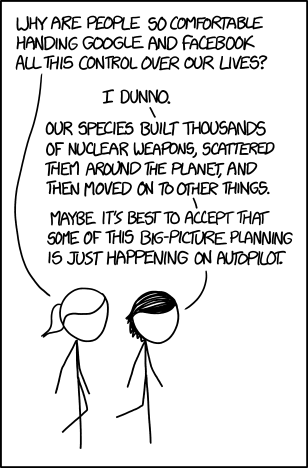
\includegraphics[width=3.5cm]{bilder/planning.png}}
}

\subsection*{Softwarelizenzen}

Über das URZ kann man als Studentin auch Lizenzen für verschiedene Programme und Betriebssysteme bekommen. Zum Beispiel Microsoft Office 365 Pro Plus. Die Uni ist Teil eines Abkommens von dem Land Baden-Württemberg mit Microsoft, wodurch alle Studentinnen sich das Office 365 Pro Plus Paket für \EUR{3.99} im Jahr holen können. Auch erwähnenswet ist Matlab, was für numerische Anwendungen ein praktisches Programm ist. Die gesamte aktuelle Liste findet ihr auf der URZ-Webseite \footnote{\url{https://public.urz.uni-heidelberg.de/service-katalog/index.html?p=software/lizenzen}}.

Außerdem gibt es diverse andere externe Dienstleister, die extra für Studentinnen besondere Konditionen anbieten. Zum Beispiel kann man bei GitHub als Studentin unbegrenzt viele private Repositories kostenlos anlegen. Häufig ist für so etwas die \emph{@stud.uni-heidelberg.de}-Adresse notwendig.

\section{Bibliotheken}
%\mathphyssecnobar{Bibliotheken}%FIXME
\begin{table*}[tb]
\centering

% Diese Tabelle wurde mühsam angeordnet. Bitte nicht umbrechen, sondern scrollen!
%~ \newcommand{\bibKIP}{}
\begin{tabular}{lll@{ -- }l@{\quad}r@{ -- }l@{ Uhr}}
\toprule
Name                                    & Adresse                                                                                                                       & \multicolumn{4}{l}{"Offnungszeiten}    \\
\midrule
\multirow{3}{*}{\gls{UB} (Ausleihe)}    & \multirow{1}{*}{\href{http://www.openstreetmap.org/?mlat=49.40966&mlon=8.70594&zoom=17&layers=M}{Plöck 107-109 (Altstadt)}}   & Mo & Fr                    & 9    & 19 \\[-0.7\defaultaddspace]
                                        & \multicolumn{1}{c}{und}                                                                                                                                                \\[-0.7\defaultaddspace]
                                        & \multirow{1}{*}{\href{http://www.openstreetmap.org/?mlat=49.41767&mlon=8.66836&zoom=17&layers=M}{INF 368, 3. Stock (Feld)}}   & \multicolumn{2}{l}{Sa}     & 9    & 13 \\
\cmidrule{1-6}
\multirow{5}{*}{\gls{UB} (Lesesaal)}    & \multirow{2}{*}{\href{http://www.openstreetmap.org/?mlat=49.40966&mlon=8.70594&zoom=17&layers=M}{Plöck 107-109 (Altstadt)}}   & Mo & Fr                    & 8:30 & 1 \\
                                        &                                                                                                                               & Sa & So                    & 9    & 1 \\[-0.7\defaultaddspace]
                                        & \multicolumn{1}{c}{}                                                                                                                                                \\[-0.7\defaultaddspace]
                                        & \multirow{2}{*}{\href{http://www.openstreetmap.org/?mlat=49.41767&mlon=8.66836&zoom=17&layers=M}{INF 368 (Feld)}}             & Mo & Fr                    & 8:30 & 22 \\
                                        &                                                                                                                               & Sa & So                    & 9    & 22 \\
\cmidrule{1-6}

\multirow{2}{*}{Mathematikon}           & \multirow{2}{*}{\href{http://www.openstreetmap.org/?mlat=49.41730&mlon=8.67580\#map=17/49.41730/8.67580}{INF 205}}            & Mo & Fr                    & 8    & 21 \\
                                        &                                                                                                                               & \multicolumn{2}{l}{Sa}     & 9    & 16 \\
\cmidrule{1-6}
\multirow{2}{*}{Physik}                 & \multirow{2}{*}{\href{http://www.openstreetmap.org/?mlat=49.41479&mlon=8.69686&zoom=17&layers=M}{Philosophenweg 16}}          & Mo & Do                    & 9    & 19 \\
                                        &                                                                                                                               & \multicolumn{2}{l}{Fr}     & 9    & 17 \\
\cmidrule{1-6}
\multirow{3}{*}{Stadtbücherei}          & \multirow{3}{*}{\href{http://www.openstreetmap.org/?mlat=49.40638&mlon=8.6866&zoom=17&layers=M}{Poststraße 15}}               & Di & Fr                    & 10   & 20 \\
                                        &                                                                                                                               & \multicolumn{2}{l}{Sa}     & 10   & 16 \\
                                        &                                                                                                                               & \multicolumn{4}{l}{Montags geschlossen!}\\
\cmidrule{1-6}
\multirow{2}{*}{Studibücherei}          & \multirow{2}{*}{\href{http://www.openstreetmap.org/?mlat=49.41082&mlon=8.70733&zoom=17&layers=M}{Schulgasse 6}}               & Mo & Do                    & 11   & 17 \\
                                        &                                                                                                                            & \multicolumn{2}{l}{Fr}     & 11   & 14 \\
\bottomrule
\end{tabular}

\end{table*}

Fachliteratur ist meistens unglaublich teuer. Um den totalen Ruin der Studierenden zu vermeiden, hat jede Universität Bibliotheken. In Heidelberg ist die \gls{UB} dreigeteilt, und zwar entsprechend der Dreiteilung der Universität. Die für euch wahrscheinlich interessanteste Literatur über Mathe, Informatik und Physik befindet sich in der Zweigstelle \gls{INF}~368, 3.~Stock.

Neben Physik-, Informatik- und Mathebüchern können hier auch medizinische Literatur und Bücher zu allen anderen Fakultäten, die im Neuenheimer Feld untergebracht sind, ausgeliehen werden. Im Hauptsitz der \gls{UB} an der Peterskirche, Plöck~107-109, und der Campus-Bibliothek in Bergheim hingegen findet sich die geisteswissenschaftliche Literatur sowie zahlreichen Jura- und VWL- Büchern. Bedingt durch diese Dreiteilung wurde in Heidelberg sehr früh ein Computersystem („\gls{HEIDI}“ \footnote{\url{http://katalog.ub.uni-heidelberg.de}}) in der UB eingeführt. Mit Hilfe von Heidi und eurer Uni-ID, die auf eurem Studiausweis steht, kann dort die gängige Fachliteratur ausgeliehen werden. Übers Internet lässt sich auch direkt nach Büchern suchen, außerdem können ausgeliehene Bücher online verlängert werden -- das kann einem durchaus den ein oder anderen Euro sparen, die Mahngebühren bei überzogenen Fristen sind nämlich empfindlich teuer. Zu Semesterbeginn finden in der UB Einführungskurse in Heidi statt, die jedoch nur bedingt sinnvoll sind, weil das System sehr übersichtlich und intuitiv aufgebaut ist und sich größtenteils selbsterklärend bedienen lässt.

So ist es bspw. möglich über die Suche festzustellen, ob ein Buch als E-Book aufrufbar ist. Der jeweilige Sucheintrag enthält dann links-unten einen \gls{Online-Ressource}-Hinweis. Auf der jeweiligen Seite des Buches findet sich dann links-oben ein Link \gls{online aufrufen}, der zu der E-Book-Version führt, nachdem du \gls{Universität Heidelberg} angewählt und dich mit deiner Uni-ID angemeldet hast.  

Wer weiterführende spezielle Fachliteratur sucht, muss sich an die Bereichsbibliotheken der einzelnen Fakultäten halten. Für Mathe- und Informatik-Literatur befindet sich die Bereichsbibliothek im Gebäude\-\gls{INF}~205 (im Erdgeschoss auf der Ostseite). Weitere Informationen und Öffnungszeiten finden sich auf der Webseite der Bereichsbibliothek\footnote{\url{https://www.mathinf.uni-heidelberg.de/bib}}. Spezielle Physikbücher stehen in der Physik-Bereichsbibliothek im Philosophenweg~16\footnote{\url{http://www.ub.uni-heidelberg.de/dezentral/bpa/standorte.html}}. Einziger Nachteil: Die zahlreichen Bücher und Spezialzeitschriften können hier nur zum Kopieren ausgeliehen werden. Wenn ein Buch in der UB ausgeliehen ist, dann lohnt es sich manchmal auch, zur Stadtbücherei in der Poststraße zu gehen. Sie wurde 1993 aufwendig umgebaut und besitzt seitdem ebenfalls ein „neues“ Computersystem. Zum Anmelden braucht man nur einen Personalausweis. Die Ausleihe ist seit dem Umbau allerdings nicht mehr kostenlos (\EUR{10}/Jahr).\\ Weitere Information kannst du auch direkt bei der Stadtbücherei einholen\footnote{\url{http://www.stadtbuecherei-heidelberg.bib-bw.de}}.

Vom Studierendenwerk gibt es zusätzlich noch die Studierendenbibliothek\footnote{\url{http://www.studentenwerk.uni-heidelberg.de/de/studibuecherei}}. Diese wie auch die Stadtbücherei eignen sich natürlich insbesondere auch dazu, neben der ganzen Studiererei einfach mal abzuschalten und zu schmökern.

\section{Arbeitsraum}
\label{sec:arbeitsraum}
Seit einigen Semestern gibt es einen betreuten studentischen Arbeitsraum in der Physik. Diesen haben wir vor allem für euch eingerichtet. Das Tolle daran ist, dass einige Tutorinnen eingestellt wurden, um euch bei Fragen und Problemen zur Verfügung zu stehen. Das läuft sehr gut und wir haben bisher viel positive Resonanz bekommen, besonders für die Tutorinnen. Das Konzept ist eine Art Bedarftutorium. Das heißt die Tutorinnen sind für eure Fragen da. Besonders Fragen und Probleme, die in den regulären Übungsgruppen keinen Platz haben, könnt ihr hier diskutieren. Oft verliert man nämlich im Übungszetteldschungel den Überblick, was wirklich wichtig ist. Genau dabei können einem aber ältere Studis helfen. Auch sollen sie dir helfen, deine Übungszettel besser zu lösen, indem sie dir hilfreiche Tipps geben. Klarerweise sollen sie dir keine Lösungen geben, sondern dich auf dem Weg dahin unterstützen.

Zu finden sind die Tutorinnen im \gls{KIP} im 2. Stock im Foyer vor den Seminarräumen bzw.\, aktuell online\footnote{\url{https://uebungen.physik.uni-heidelberg.de/arbeitsraum}}. Während der Vorlesungszeit sitzen dort montags bis freitags von 13 bis 19 Uhr bis zu zwei Tutorinnen, die ihr mit Hilfe eines großen Plakats erkennen könnt. Neben einer großen Auswahl Standardlehrbüchern gibt es dort auch eine Kaffeemaschine und einen Wasserkocher, wo ihr Kaffee und Tee zu günstigen Preisen bekommen könnt.

Falls du also mal an einem Zettel verzweifelst, komm einfach vorbei und lass dir helfen.

\newpage
\section{Was tun bei Problemen}
\label{dschungel}
Da seid ihr also: ordentlich immatrikuliert, auch schon eine Bleibe gefunden (zumindest vorläufig), möglicherweise bereits Bekanntschaft mit diversen Ämtern und Behörden geschlossen. Und nun kann es eigentlich losgehen mit dem „lustigen Studentinnenleben“. Oder?

Aber was ist das eigentlich, studieren? Wie wird das Studium im ersten Semester aussehen? Wie lernt man denn an der Uni, wenn einem niemand so richtig vorschreibt, was wann wie zu machen ist? Überall hört man von Studiengebühren -- betrifft mich das eigentlich? Und wie ist das mit dem BAfÖG? Wann muss ich meine ersten Prüfungen ablegen? Wie kann ich Studium und Job unter einen Hut bringen? Bleibt neben dem Studium überhaupt noch Zeit, etwas anderes zu machen?

Was im Weltall gilt, gilt auch in der geistigen Galaxie: Don't panic! Der Überblick, den ihr jetzt noch nicht habt, stellt sich noch ein. Vor allem seid ihr nicht allein. Ein Anliegen dieses Heftes ist es, euch die Anlaufstellen aufzuzeigen, wie z.\,B.\ die Zentrale Studienberatung, Sozial- und Rechtsberatung, oder die Psychosoziale Beratungsstelle des Studierendenwerks\footnote{Überblick über die einzelnen Beratungsangebote:\\\url{http://www.uni-heidelberg.de/studium/imstudium/beratung.html}}.

Worüber ihr euch klar werden solltet, ist, was ihr euch vom Studium erwartet. Fragt euch also: Warum studiere ich? Welches Berufsziel schwebt mir vor? Warum gerade dieses Fach? Ihr müsst diese Entscheidungen für euch selbst treffen und Prioritäten setzen -- der Stundenplan bietet keine Anleitung dazu, die eigenen Fähigkeiten und Erwartungen im Studium umzusetzen.\enlargethispage{\baselineskip}%FIXME

%\begin{minipage}{1.5\textwidth}
%\hspace{-5mm}
%        \includegraphics[width=6cm]{bilder/dschungelbuch_1.png}
%        \hspace{10mm}
%        \includegraphics[width=6cm]{bilder/dschungelbuch_2.png}\\\vspace{5mm}
%\end{minipage}

%\section{Die kleine BAföG-Liste}
\mathphyssecnobar{Die kleine BAföG-Liste}%FIXME

\paragraph{Soll ich BAföG beantragen?}
JA! Ob du anspruchsberechtigt bist, lässt sich nur schätzen. Vom BAföG sind 50\% Zuschuss, die andere Hälfte zinsloses Darlehen. Zurückzuzahlen muss man es frühestens drei Jahre nach Studienabschluss, aber nur ab einer bestimmten Einkommenshöhe. Rückzahlungsaufschub ist jederzeit ohne Nachteile möglich!

\paragraph{Wie viel gibt es und wie lange und ab wann?}
Maximal \EUR{648} (ohne Kind, abhängig von Miet(e)verhältnis, Einkommen der Eltern, eigenem Vermögen, Krankenversicherung, Geschwistern, etc.) Die Förderungsdauer richtet sich nach der Regelstudienzeit (Bachelor und konsekutiver Master = 6 + 4, aber es gibt fachspezifische Ausnahmen), Anspruchszeit zählt ab Immatrikulation und ist nicht aufsparbar! Die Auszahlung geschieht in der Regel erst, wenn Bescheid eingegangen ist, bei dringender Bedürftigkeit ist ggf. Vorschuss (in voller BAföG-Höhe, der hinterher verrechnet wird) möglich.

\paragraph{Wo und bis wann muss ich den Antrag stellen?}
Das geht beim BAföG-Amt des Studentenwerks im Marstallhof 3 je Mo.\ -- Fr.\ 8 – 18 Uhr. Kurzberatung im Neuenheimer Feld gibt es Mo.\ – Do.\ 10.00 -- 17.00 Uhr und Fr.\ 10.00 -- 15.00 Uhr. Das macht man am besten sobald man die Immatrikulationsbescheinigung hat, denn BAföG gibt es erst vom Antragsmonat an, wobei der frühestmögliche Termin der Semesteranfang ist.

\paragraph{Was muss ich beim Antrag beachten?}
Antrag so früh wie möglich stellen, weil es teilweise zu langen Bearbeitungszeiten kommen kann. Der Antrag sollte idealerweise vollständig sein, da so Rückfragen entfallen und der Antrag schneller bearbeitet werden kann. Ansonsten gilt: lieber schnell beantragen und Papiere nachreichen. Die Angaben sollten wahrheitsgemäß sein, denn das Amt kann die Finanzdaten prüfen.

\paragraph{BAföG und nun? Was sonst noch zu beachten wäre.}
Man muss nach dem vierten Fachsemester seine Studienleistungen bescheinigen lassen! Familiäre und persönliche wirtschaftliche Veränderungen immer sofort melden (Schwester/Bruder in Ausbildung/Arbeit, Arbeitslosigkeit, etc.) Es gibt auch Auslands-BAföG und viele sonstige Ausnahmen, zu denen man sich am besten beraten lässt! Es kann sich lohnen! Zuverdienst bis maximal \EUR{4\,880} Brutto im Jahr oder \EUR{450} im Monat (mit vielen Ausnahmen).\\[5mm]

\noindent Abschließend: Nutzt die Sprechstunde vom Sozialreferat des \gls{StuRa} (Mi.\ und Fr.\ 11 -- 13 Uhr). Die helfen Euch beim Antrag, erklären Ausnahmen, geben Tipps (um spätere Probleme zu vermeiden, bei denen sie natürlich auch helfen).

% !TEX ROOT = ../ersti.tex
\section{Studium im Ausland}
Man hört immer wieder von den tollen Erfahrungen und Möglichkeiten, die ein Studium im Ausland bietet. Die Leute schwärmen davon, wie schön es an der Uni so-und-so war. Aber wie kommt man überhaupt dahin?

In den Bachelor-Studienordnungen der Physik und der Mathe heißt es, „Bei der Anerkennung von Studienzeiten, Studien- und Prüfungsleistungen, die außerhalb Deutschlands erbracht wurden, sind die von Kultusministerkonferenz und Hochschulrektorenkonferenz gebilligten Äquivalenzvereinbarungen sowie Absprachen im Rahmen von Hochschulpartnerschaften zu beachten. Bei Zweifeln an der Gleichwertigkeit kann die Zentralstelle für ausländisches Bildungswesen gehört werden.“ Das ist nicht sonderlich hilfreich, wenn man sich nicht unbedingt durch Tonnen von Gesetzestext quälen will. Auf der Homepage der jeweiligen Fakultät findet ihr eine Liste von Unis, mit denen Austauschprogramme laufen (die also anerkannt werden), einige generelle Infos und ein paar Erfahrungsberichte, die ihr bei Interesse anschauen solltet. Die Gleichwertigkeit von Studienleistungen muss allerdings nicht von euch überprüft werden, die Beweispflicht liegt bei der Fakultät. Lasst euch also nicht beirren und hört im Zweifel die Veranstaltung im Ausland einfach, die sollen erst mal zeigen, dass das nicht das gleiche war.

Allerdings sollte ein Auslandssemester im Moment nicht euer erstes Problem sein -- während der ersten beiden Semester ist es ganz einfach fachlich nicht möglich. Bis zur Einführung der Bachelor- und Masterstudiengänge konnte man (wenigstens in der Mathe) an diesen Programmen nur nach abgeschlossenem Grundstudium teilnehmen, inzwischen wird der Zeitraum letztes Jahr Bachelor/erstes Jahr Master empfohlen. Das bedeutet, dass ihr nach dem zweiten Semester damit beginnen solltet, euch umzuschauen, insbesondere in Bezug auf Bewerbungsvoraussetzungen und -fristen.

AuslandsBAföG müsst ihr übrigens separat beantragen, die Zu\-stän\-dig\-keit dafür hängt vom jeweiligen Ausland ab, eine Liste der zuständigen Ämter findet man z.B. unter \url{AuslandsBAfoeG.de}. In Heidelberg kann man sich auch direkt an das Dezernat Internationale Beziehungen (früher Akademisches Auslandsamt, AAA)\footnote{\url{http://www.uni-heidelberg.de/studium/kontakt/auslandsamt/}} wenden, das ihr in der Seminarstraße 2 findet. Ihr müsst dann ins Zimmer 139.

\paragraph{Öffnungszeiten} Mo. -- Do. 10 -- 15 \qquad Fr. 10 -- 13

Sehr wichtig ist noch zu wissen, dass man Urlaubssemester beantragen kann, damit die Fachsemesterzahl (vorallem wichtig für alle, die Inlands-BAföG erhalten) nicht weiterläuft. Dafür läuft die Hochschulsemesterzahl weiter. Man kann sich dann die im Ausland erworbenen \gls{LP} (nach Absprache mit dem Prüfungssekreteriat) anrechnen lassen.

Für das Urlaubssemester ist die Studierendenadministration in der Seminarstraße 2 zuständig. Mehr Infos und das Formular zum Urlaubssemester findet ihr unter:
\url{https://www.uni-heidelberg.de/studium/imstudium/formalia/beurlaubung.html}


% !TEX ROOT = ../ersti.tex
\section{Weitere Angebote}

\subsection{Mathematik-Mentorinnenprogramm \\Upstream}
Das Interdisziplinäre Zentrum für Wissenschaftliches Rechnen (IWR) an der Uni Heidelberg bietet seit 2013 mit Upstream\footnote{\url{http://www.mathcomp.uni-heidelberg.de/programs/upstream}} ein Mentorinnenprogramm für Mathematik-interessierte Frauen. Upstream ist ein Netzwerk für junge Mathematikerinnen in allen Stufen der Ausbildung -- von Schülerinnen ab der 10. Klasse, Studentinnen, Doktorandinnen, Nachwuchswissenschaftlerinnen bis hin zu Professorinnen. In regelmäßigen Abständen organisieren wir Meet\,\&\,Greet-Treffen, Public Lectures, Diskussionsrunden und Workshops zu Themen, in denen Schlüsselqualifikationen und studiengangsspezifische Inhalte vermittelt werden. Dabei nehmen erfahrene Mathematikerinnen die Mentorinnenrolle ein. Sie stehen den Teilnehmerinnen zur Seite, beraten und beantworten Fragen rund um das Studium und das Berufsleben.

Wenn du Mitglied werden willst, schicke einfach etwa eine halbe Seite Motivationsschreiben per E-Mail an: upstream@iwr.uni-heidelberg.de. Die Aufnahme in das Programm ist nicht an Noten oder Wettbewerbserfolge geknüpft; Wir suchen vor allem begeisterte Mathematikerinnen auf allen Ebenen.

\subsection{Kooperationsabkommen mit der \\Universität Mannheim}
Zwischen der Universität Heidelberg und der Universität Mannheim gibt es ein Kooperationsabkommen, was Studierenden in Mathematik, Informatik und Physik ermöglicht, kostenlos als Gaststudentin Vorlesungen an Fakultät für Wirtschaftsmathematik und Wirtschaftsinformatik zu hören und sich hier in Heidelberg anrechnen lassen. 
Somit kann man das vielfältige Vorlesungsangebot nutzen und insbesondere Module wie Kryptographie, angewandte Algebra und Spieltheorie belegen, die so nicht in Heidelberg angeboten werden.

\subsection{Kooperation mit dem Theater und Orchester Heidelberg}
Seit einiger Zeit ist es geplant, mit dem Theater und Orchester Heidelberg eine Kooperation einzugehen, um eine Art Theaterflatrate anzubieten. Die Grundidee: Jede*r Studierende zahlt mit dem Semesterbeitrag einen geringfügigen Pauschalbetrag. Dafür wird ein bestimmtes Kontingent an Karten reserviert, auf das Studierende kostenfrei zugreifen können. 
Da der Testlauf erst mit Beginn des Wintersemesters am 01. Oktober startet, gibt es noch keine verbindliche Auskünfte. Sobald alles festgelegt ist, bekommti ihr alle relevanten Infos.


%%%%%%%%%%%%%%%%%%%%%%%%%%%%%%%%%%%%%%%%%%%%%%%%%%%%%%%%%%%%%%%%%%%%%%%%%%%%%
\chapter{\dots und in der Stadt}
% !TEX ROOT = ../ersti.tex
\section{Wohnen in Heidelberg}

Wie in jeder Unistadt, so ist es auch in Heidelberg schwer, zu Anfang des Semesters ein Zimmer zu finden, das bezahlbar ist und möglichst zentral liegt. Im Durchschnitt muss man in Heidelberg mit Lebenshaltungskosten von ca. \lebenshaltungskosten (inklusive Miete) pro Monat rechnen.

\begin{figure*}[b]
    \centering
    \begin{subfigure}{.3\textwidth}
    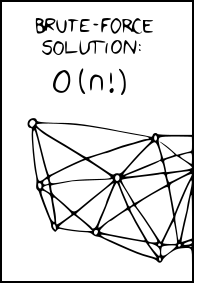
\includegraphics[height=4.5cm]{bilder/travelling_salesman_problem_1.png}
    \end{subfigure}
    \begin{subfigure}{.3\textwidth}
    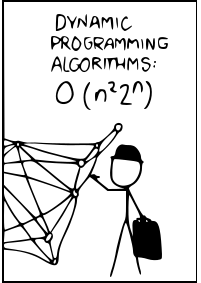
\includegraphics[height=4.5cm]{bilder/travelling_salesman_problem_2.png}
    \end{subfigure}
    \begin{subfigure}{.3\textwidth}
    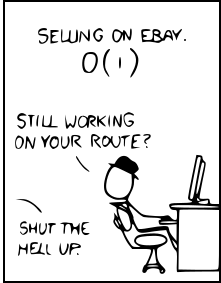
\includegraphics[height=4.5cm]{bilder/travelling_salesman_problem_3.png}
    \end{subfigure}
\end{figure*}

Am günstigsten wohnt man immer noch im Studentenwohnheim, dort muss man mit Mieten von ca. \studentenwohnheim pro Monat rechnen. Eine frühzeitige Bewerbung ist hier dringend notwendig. Auch WG-Zimmer sind teilweise recht günstig zu bekommen, in der Regel jedoch teurer als ein Zimmer im Wohnheim und oft nicht lange im Voraus zu reservieren.

Die Idee, eine eigene WG zu gründen, liegt meist sehr nahe, jedoch wird man schnell merken, dass das gar nicht so einfach ist. Oft werden Ehepaare ohne Kinder bevorzugt oder ein Zimmer entpuppt sich als Durchgangszimmer. Egal, für was ihr euch entscheidet: plant viel Zeit ein und lasst nicht locker!

Nun aber zur konkreten Zimmersuche: es gibt mehrere Möglichkeiten, ein Zimmer in Heidelberg zu finden. Das Studierendenwerk bietet mehrere Anlaufstellen: In der Altstadt das Info-Café International in der Triplex-Mensa direkt am Uniplatz, im Neuenheimer Feld im Infocenter der Zentralmensa. In den Mensen, aber auch in den einzelnen Instituten empfiehlt es sich, die schwarzen Bretter abzuklappern und nach privaten Aushängen Ausschau zu halten oder selbst Anfragen anzuhängen. Weitere gute Quellen für Zimmerangebote sind natürlich die regionalen Zeitungen. Das wären u.a. „Sperrmüll“, erscheint immer dienstags und freitags, und die Rhein-Neckar-Zeitung, mittwochs und samstags mit großem Immobilienteil. %Aufpassen müsst ihr bei Makler-Vermittlungen, hier müsst ihr zusätzlich zwischen %ein und zwei Monatsmieten Provision zahlen. Eine eigene Anzeige kann natürlich nie schaden. Zu guter Letzt gibt es noch das Internet, das eine Fülle an Portalen\footnote{z.B. \url{wg-gesucht.de}} zur Wohnungssuche bietet.


\subsubsection{Wohnheime}

\begin{figure*}[t]
    \centering
    \begin{subfigure}{.2\textwidth}
    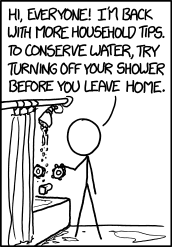
\includegraphics[height=4.5cm]{bilder/household_tips_1.png}
    \end{subfigure}
    \begin{subfigure}{.25\textwidth}
    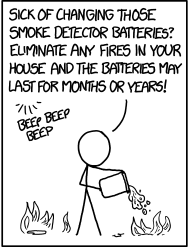
\includegraphics[height=4.5cm]{bilder/household_tips_2.png}
    \end{subfigure}
    \begin{subfigure}{.2\textwidth}
    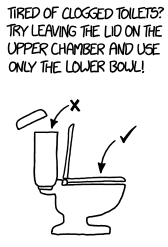
\includegraphics[height=4.5cm]{bilder/household_tips_3.png}
    \end{subfigure}
    \begin{subfigure}{.28\textwidth}
    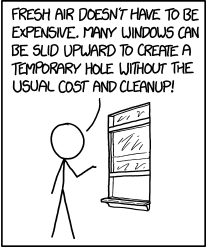
\includegraphics[height=4.5cm]{bilder/household_tips_4.png}
    \end{subfigure}
\end{figure*}

In und um Heidelberg gibt es ca. 50 Wohnheime des Studierendenwerks, im Wintersemester werden ca. ein Fünftel aller dieser Zimmer neu vermietet. Die Auswahl erfolgt nach sozialen Kriterien wie zum Beispiel Heimatferne, Verdienst der Eltern, Wohnverhältnisse usw. Die Wohnzeit ist auf sechs Semester begrenzt, aber es gibt viele Möglichkeiten, diese zu verlängern, zum Beispiel durch Sonderaufgaben im Wohnheim, Härtefälle etc. Die maximale Wohnzeit kann auf insgesamt zehn Semester ansteigen, was durchaus vorkommt. Je nach Wohnheim gibt es Einzelzimmer mit Stockwerksküche und -Bad, die ihr dann mit jeweils 15-20 Leuten teilt (was mittlerweile aber eher selten ist), Einzelzimmer in 2er, 3er oder 4er WGs oder sogar Einzelappartments. Die Zimmer sind in der Regel nicht sehr groß (11--16 \squaren\metre), aber ausreichend. Nachteile von Wohnheimen können die teilweise sehr unterschiedlichen Vorstellungen von Hygiene sein, ein hoher Lärmpegel und immer wieder neue Überraschungen. Allerdings bietet ein Wohnheim vor allem für Leute, die neu in der Stadt sind, den großen Vorteil sehr schnell viele Leute kennen zu lernen, außerdem muss man sich um Reparaturen nicht selbst kümmern. Es gibt keine konkreten Bewerbungsfristen. Die Bewerbung sollte allerdings bis 1. Juli für das Wintersemester und bis 1. Januar für das Sommersemester eingegangen sein, weil dann mit der Zimmereinteilung und dem Versand der Mietverträge begonnen wird. Später eingehende Bewerbungen haben weitaus geringere Chancen und Auswahlmöglichkeiten. Antragsformulare gibt es in den Infocentern des Studierendenwerks oder im Internet.\footnote{\url{http://www.studentenwerk.uni-heidelberg.de}} Dort gibt es auch eine vollständige Liste aller Wohnheime des Studierendenwerks. Auch private, kirchliche oder sonstige Träger bieten Zimmer in Wohnheimen an, für diese müsst ihr euch direkt beim Wohnheim bewerben, nicht beim Studierendenwerk. Eine Liste findet ihr aber beim Studierendenwerk.\footnote{\url{http://www.stw.uni-heidelberg.de/sites/default/files/download/pdf/wo-in-hd-andere-traeger-de.pdf}}

% !TEX ROOT = ../ersti.tex
\newcounter{zahl}
\newcommand{\place}[4]{\item[(\stepcounter{zahl}\thezahl) #1](#2)\\ #3\\\emph{Preis:} #4}

% Indikator für Frauenanteil? Nein!

\section{Bars, Kneipen \& Diskotheken}
$\star$ teuer, $\star\ \star$ noch teurer, $\star\ \star\ \star$ extrem teuer

% trim=l b r t
%\hspace*{-6mm}
\begin{figure*}
\altstadtkarte
\end{figure*}

\subsection{In der Altstadt:}
\begin{description}

%   \place{Alfredo}{Untere Straße}{Wirklich sehr leckere Pizza, der Chef sorgt für den echt italienischen Flair.}{$\star$}

    \place{Destille}{Untere Straße 16}{Besondere Shots, die jede in Heidelberg mal probiert haben sollte („Warmer Erpel“ \& „Gehängter“). Selbst an Tagen an denen die Untere Straße leer ist, tanzen hier Leute auf den Tischen.}{$\star\ \star$}

    \place{Sonderbar / „Betreutes Trinken“}{Untere Straße 13}{Jede nur erdenkliche Form von Absinth, auch viel guten Rum und Whisky. Immer ordentlich was auf die Ohren (Hard \& Heavy). Keine Angst vor dem Wirt, einfach nicht auf den Mund gefallen sein. Oft sehr voll und vollgeräuchert.}{$\star\ \star$}

    \place{Eckstein}{am Fischmarkt 3}{Abgefahrene Kneipe. Je nach Wochentag ändert sich das Programm. Es gibt jedoch immer einen Kicker und reichlich Platz. Drei Mal wöchentlich Zaubershows.}{$\star\ \star$}

    \place{Mohr}{Untere Straße 3}{Spät abends meist so voll, dass man gar nicht mehr rein kommt. Drinnen wird dafür allerdings auf den Tischen getanzt. Donnerstags gibts zur Ladies’ Night kostenlosen Sekt für die Damen.}{$\star\ \star$}

    \place{Palmbräugasse}{Untere Straße}{Hier gibts das selbstgebraute Palmbräu. Palmen gehören zwar nicht typisch zu Heidelberg, aber die Schnitzel in der Palmbräugasse.}{$\star\ \star\ \star$}

    \place{Reichsapfel \% Lager}{Untere Straße 35}{Sehr geräumig. Moderner Vorderbereich und urigere Atmosphäre im hinteren Teil, welcher über den Innenhof zugänglich ist. Dort findet man oft Platz, wenn sonst alles voll ist.}{$\star\ \star$}

    \place{Mels}{Heiliggeiststr. 1}{Gewölbekeller, in dem seit Jahren die selbe Musik läuft, aber zumindest weiß man dann, was einen erwartet. Haben unter der Woche immer sehr gute Spezialangebote z.B. Dienstags 123-Party (Bier \EUR{1}, Weizen \EUR{2}, Cocktails \EUR{3}).}{$\star\ \star$}

    \place{Cave 54}{Krämergasse 1}{(Deutschlands ältester) Jazzkeller. Kostet am Wochen\-ende Eintritt, hat dafür allerdings noch nach 3 Uhr geöffnet.}{$\star\ \star$}

    \place{Coyote Café}{Hauptstraße}{Einer der Orte, um eine Kneipentour durch die Altstadt starten zu lassen. Weizenbier, Cocktails und Shots sind brauchbar und brauchen nicht ewig. Am späteren Abend gibt es häufig eine Happy Hour, bei der Cocktails nur die Hälfte kosten.}{$\star\ \star$}

    %\place{Hard Rock Cafe}{Hauptstraße 142}{Montags Bier für \EUR{1}, ab 18 Uhr Cocktails für \EUR{4}. Musik wie man es erwartet, durchgehend Rock.}{$\star$}
    \place{Ben's Burgerbar (ehem. Hard Rock Cafe)}{Hauptstraße 142}{Ab 18 Uhr Cocktails für \EUR{4}. Musik wie man es erwartet, durchgehend Rock.}{$\star$}

%    \place{Havanna}{Neckarstaden 24}{Cocktailbar mit Möglichkeit zum Salsa tanzen.}{$\star\ \star\ \star$}

    \place{Hemmingways}{Fahrtgasse 1}{Hier lässt es sich das gesamte Jahr draußen sitzen, dank warmen Decken und Heizstrahlern. Außerdem kann man wunderbar den Neckar beobachten.}{$\star\ \star$}

    \place{Karl}{Lauerstraße 7-9}{Kneipe mit Billardtisch und Dartscheibe. Manchmal mit Live-Musik.}{$\star\ \star$}

    \place{Karlstorbahnhof}{Am Karlstor\,/\,S-Bahnhof Altstadt}{Richtig gute Diskothek (Nicht nur; im Gebäude gibts auch Theater, Lesungen etc. -- viel Kultur) mit sehr variabler Musik. Was zum tanzen und weniger zum trinken, denn die Preise können sich meistens sehen lassen, genauso der Eintritt}{$\star\ \star\ \star$}

    \place{Marstall}{Marstallhof}{Keine typische Kneipe, vielmehr Mensa mit Bier. Trotzdem gut geeignet, um sich zu treffen, zum Vorglühen und entscheiden, wo die weitere Party ihren Anfang nehmen soll.}{$\star$}

    \place{Maxbar}{Marktplatz 5}{Schöne Kneipe, bei der man Tagsüber auf dem Marktplatz sitzen kann.}{$\star\ \star$}

    \place{Medoc}{Bismarckplatz}{Cafe Restaurant das für ca. \EUR{5} aufwärts wechselnde Mittagsgerichte anbietet. Man kann draußen sitzen und den Betrieb auf dem Bismarckplatz beobachten.}{$\star\ \star$}

    \place{Orange}{Ingrimmstraße 26a}{Eine Kneipe wie ein Wohnzimmer. Eng aber gemütlich. Bietet sehr leckeres Bier aus Tschechien an, ist aber leider eher verraucht. Es gibt sogar Brettspiele.}{$\star\ \star$}

    \place{Regie}{Theaterplatz}{Riesenauswahl an Cocktails, die nach Filmen benannt und meist recht schick dekoriert sind. Cooles Specials- und Aktionensystem und leckere Flammkuchen}{$\star\ \star\ \star$}

    \place{Tangente}{Kettengasse 23}{Hoher Juristinnenanteil und teils ältere Menschen. Türsteher und Gesichtskontrolle, dafür aber kein Eintritt. Hier kann man bis in die frühen Morgenstunden tanzen, man sollte allerdings keine Platzangst haben.}{$\star\ \star$}

    \place{Vater Rhein}{Untere Neckarstraße 20}{Legendär für seine \EUR{2,20}-Spaghetti bis zwei Uhr. Hier lässt sich der Abend gemütlich ausklingen. Stammkneipe vieler Stammtische in Heidelberg.}{$\star$}

	\place{Vetters}{Steingasse 9}{Nicht zum Bleiben, aber für die Maß to go. Gibts da für \EUR{3} (+ Pfand), schmeckt hervorragend. Ansonsten gutbürgerliche Küche, älteres Klientel und viele Touristen. Brauen das Bier mit dem höchsten Stammwürzegehalt der Welt (33\%).}{$\star\ \star$}

    \place{Dubliners}{Hauptstraße 93}{Irish Pub mit Karaoke und Quiz-Nights (donnerstags).}{$\star\ \star\ \star$}

    \place{Shooter Stars}{Heugasse 1}{Shotbar mit einer Auswahl von mehr als 300 verschiedenen Shots. Hier kann man beispielsweise eine „Nachklausur“ bestellen.}{$\star\ \star$}

    \place{Metropol Billard}{Kettengasse 21}{Billard-Kneipe mit günstigen Cocktails.}{$\star$}

    \place{Boho}{Kettengasse 11}{Bar in Neon-Optik. Hier werden überwiegend Charts gespielt.}{$\star\ \star$}
\end{description}



%%%%%%%%%
\subsection{In den Stadtteilen:}
\begin{description}

    \place{Bar 133}{Wohnheim \gls{INF} 133}{Wohnheimsbar, eigentlich nur für Bewohner der 1xx Wohnheime. Mittwochs und sonntags geöffnet mit gutem Angebot, günstigen Cocktails und Tischkicker.}{$\star$}

	\place{Comabar}{Comenius-Haus}{Bar des Comenius-Hauses direkt am Bunsengymnasium. Dienstags und Donnerstags geöffnet, super Team, günstige Cocktails, Kicker und Tischtennisplatte vorhanden. Definitiv empfehlenswert.}{$\star$}

%    \place{Breidenbach Studios}{Hebelstraße 18}{Absoluter Hipster-Laden: Ehemalige Gasflaschenhandlung, die zu einem Künstlerhaus und Coworking-Space umgebaut wurde. Hier finden immer wieder großartige Partys statt.}{$\star\ \star\ \star$}

    \place{Cappuchino}{Bergheimer Straße 8}{Hippe Mischung von Kaffeehaus mit lautem Elektro.}{$\star\ \star$}

    \place{Gilberts Goldener Adler}{Handschuhsheimer Landstraße 96}{Ist eigentlich ein Restaurant, hat im Sommer aber auch einen netten Biergarten. Die Portionen sind groß und lecker. Stammlokal einiger Matheprofs.}{$\star\ \star$}

    \place{Halle 02}{Bahnstadt}{Electro-Freunde werden hier ihren Spaß haben, es gibt aber auch viele Mainstream Partys. Meistens sind diese auch recht voll und es herrscht gute Stimmung. Regelmäßig spielen hier bekanntere Bands.}{$\star\ \star$}

    \place{O'Reilly's}{Brückenkopfstraße 1}{Irish Pub mit Karaoke und Quiz-Nights.}{$\star\ \star\ \star$}

    \place{P11}{Am Römerkreis}{Nettes Café, das Abends bis etwa eins Barbetrieb hat. Trotz der Nähe zum Römerkreis angenehme Atmosphäre. Geile Tapete! Hier kann man auch im Sommer draußen sitzen.}{$\star\ \star$}

    \place{Villa Nachttanz}{Im Klingenbühl 6}{Alternativer Kulturverein -- rechnet mit allem außer Mainstream. Sehr günstig, mit Lagerfeuer im Garten. Lohnt sich jedes mal.}{$\star$}

    \place{Ziegler}{Bergheimer Straße 1}{Kneipe mit Disco, welche allerdings Eintritt kostet und auch sonst recht hohe Preise hat. Oft auch Live Musik}{$\star\ \star\ \star$}

    \place{Zwitscherstube}{Blumenstraße 25}{Urige Kneipe mit Alt, Kölsch und original Underberggürtel. Hier kommen vor allem Fußballfans auf ihre Kosten. Wenn kein Fußball läuft kann man super Skat spielen.}{$\star$}
\end{description}
%\section{Geschichte der Ruprecht-Karls-Universität Heidelberg}
\label{geschichte}
Die Ruperto Carola wurde im Jahre 1386 mit päpstlicher Genehmigung von Kurfürst Ruprecht I. als Ruprechts-Universität Heidelberg gegründet. Sie ist die Dritte im Heiligen römischen Reich deutscher Nation nach Prag und Wien, also die älteste in den Grenzen des heutigen Deutschlands. Aufgrund der Spaltung der Kirche war es nötig geworden, eine Ausbildung eigener Theologen zu ermöglichen, da Sorbonne-Absolventen nicht mehr im römischen Reich in kirchliche Dienste treten durften. Marsilius von Inghen, der Gründungsrektor, wegen der Kirchenspaltung aus Paris geflohen, eröffnet die Universität im Oktober 1386 mit einer feierlichen Messe. Die Anfänge der Universität sind durch erhebliche Raumprobleme gekennzeichnet: Kirchen und Klostersäle werden für Vorlesungen genutzt. Erst später können eigene Gebäude für die Lehre errichtet werden. Im Zuge der Universitätsgründung werden die Stiftsbibliotheken der umliegenden Klöster vereinigt, um eine einigermaßen solide Ausbildung zu gewährleisten; die Büchersammlung wird dabei kontinuierlich erweitert (zum Beispiel durch vererbte Bestände der Augsburger Handelsfamilie Fugger) und im 16. Jahrhundert zur Bibliotheca Palatina vereinigt.

1556 wird die Universität im Zuge der Reformation in eine evangelische Landeshochschule umgewandelt. Kurfürst Ottheinrich führt normale bürgerliche Kleidung statt der sonst üblichen geistlichen Tracht für Studierende ein. Auch die finanzielle Situation verbessert sich stark durch die Übertragung von Kirchengut an die Universität. Später wird die Universität sogar als calvinistische Hochschule im „deutschen Genf“ bezeichnet. So blüht sie bis 1618 auf, die Studierendenzahlen wachsen, auch wenn die Universität im Vergleich zu anderen deutschen Universitäten immer noch zu den kleinen zählt.

\marginpar{
    \centering{
        \vspace{-50mm}
        \includegraphics[width=3cm]{bilder/a_wise_man_once_said_1.PNG}\\\vspace{13mm}
        \includegraphics[width=3cm]{bilder/a_wise_man_once_said_2.PNG}\\\vspace{13mm}
        \includegraphics[width=3cm]{bilder/a_wise_man_once_said_3.PNG}\\\vspace{13mm}
        \includegraphics[width=3cm]{bilder/a_wise_man_once_said_4.PNG}\\\vspace{13mm}
        \includegraphics[width=3cm]{bilder/a_wise_man_once_said_5.PNG}\\\vspace{13mm}
        \includegraphics[width=3cm]{bilder/a_wise_man_once_said_6.PNG}\\\vspace{13mm}
    }
}

Während des 30-jährigen Kriegs wird die Universität ziemlich stark beschädigt und der Lehrbetrieb muss immer wieder unterbrochen werden bis sie schließlich 1652 wiedereröffnet wird. Doch der Frieden hält nicht lange an. Im Zuge des Pfälzer Erbfolgekrieges wird die ganze Stadt Heidelberg verwüstet. Die Bibliotheca Palatina wird als Kriegskostenersatz an den Papst verschenkt. 

%% der lehrbetrieb wurde eingestellt und eigentlich gabs die Uni nicht. Davon erholt sich die Universität nur sehr langsam.

Mitte des 18. Jahrhunderts beginnen sich die Naturwissenschaften zu etablieren. Zuerst als Teil der philosophischen Fakultät entsteht 1752 der Lehrstuhl für Mathematik und Experimentalphysik. Diese Entwicklung setzt sich 1802 mit dem Übergang Heidelbergs an Baden fort. Die Universität erweitert nach dem ersten Großherzog von Baden ihren Namen zu „Ruprecht-Karls-Universität Heidelberg“. Sie ist von jetzt an staatlich finanziert und wird komplett reorganisiert. Die Naturwissenschaftlich-Mathematische Fakultät trennt sich von der Philosophischen und entwickelt sich vor allem unter dem Einfluss von Robert Bunsen, Gustav Kirchhoff und Hermann von Helmholtz. Georg Wilhelm Friedrich Hegel lehrt zwei Jahre an der philosophischen Fakultät, die medizinische Fakultät zieht Patienten aus aller Welt an. Trotzdem wird Heidelberg vor allem als juristische Universität gesehen. Auch kommt es in dieser Zeit zu Entwicklungen in der Frauengleichstellung. Im Jahr 1895 promoviert Katharina Windscheid als erste Doktorandin in Heidelberg. 1900 wird Georgine Sexauer als erste Studentin immatrikuliert und 1923 wird Gerta von Ubisch als Professorin für Botanik habilitiert.

Im 20. Jahrhundert setzt sich dieser Trend fort. Heidelberg ist eine weltoffene und liberale Universität, an der man auch eine große Zahl von ausländischen Studierenden findet. Das interdisziplinäre Gespräch wird gesucht, was der Uni ihren typischen „Heidelberger Geist“ verleiht, der in der Weimarer Republik auch häufig als demokratischer Geist bezeichnet wird.

Trotzdem wird die Studierendenschaft im Verlauf des 20. Jahrhunderts immer radikaler und mit dem Erstarken des Nationalsozialismus werden viele Professoren und Professorinnen entlassen und Studierende aus politischen und rassistischen Gründen ausgeschlossen. Bei der Bücherverbrennung auf dem Universitätsplatz 1933 nehmen viele Mitglieder der Universität aktiv teil; die Ruperto Carola ist als braune Universität verrufen. Die Athene wich dem Hakenkreuz, der lebendige Geist dem deutschen. % Diese Gender-Form von ProfessorInnen wurde wegen dem geschichtlichen Kontext gewählt. 

Nach dem zweiten Weltkrieg ist die Universität äußerlich zerstört, gravierender sind jedoch die Schäden die durch die nationalsozialistische Ideologie verbleiben. Der inneren Erneuerung widmeten sich maßgeblich Karl Jaspers und Karl Heinrich Bauer, die eine neue Satzung ausgearbeitet und in den folgenden Jahren die Universität stark erweitern. 

Trotz aller wissenschaftlichen Erneuerung bleibt das reaktionäre Geflecht an der Universität erhalten - Athene hat ihren Platz zurück erobert, doch der lebendige freie Geist ist nicht zurück gekehrt. Gegen diese Verkrustungen begehrt die Studierendenbewegung Ende der 60er Jahre auf. Mit der polizeilichen Räumung von besetzten Universitätsgebäuden und Verhaftung von Studierenden findet diese Bewegung in Heidelberg wie auch ganz Deutschland ein jähes Ende. Als Reaktion und Bestrafung wurden studentische Mitbestimmungsrechte massiv beschnitten und seit dem nur teilweise wieder eingeführt (hier fehlt das - Verweis auf HOPO artikel).

Die Universität gewinnt stetig Studierende und wird mit der Erschließung des Neuenheimer Feldes stark erweitert. Bis zum Jubiläumsjahr 1986 wächst die Zahl der Studierenden auf ca. 27\,000 an. Heidelberg erarbeitet sich in Deutschland und darüber hinaus einen Ruf als forschungsstarke Universität.

Die neuesten Entwicklungen stammen aus dem Jahr 2007. Seitdem darf sich die Universität „Exzellenzuni“ nennen, denn ihr Zukunftskonzept „Heidelberg: Realising the Potential of a Comprehensive University“ wurde als förderungswürdig ausgewählt. 

%\section{nightline}
\section{Nightline}%FIXME
Die Nightline ist eine telefonische Anlaufstelle von Studierenden für Studierende. Jede kann bei uns anrufen oder eine Mail schreiben, um über alles, was sie gerade beschäftigt, anonym und vertraulich zu reden. Egal ob Ersti oder Doktorandin, ob 18 oder 48 Jahre alt, egal, ob jemand einfach nur kurz etwas loswerden will oder gerade alles über einem zusammenbricht. Die Nightline bietet die Möglichkeit zum offenen Gespräch am späten Abend und nachts, wenn belastende Gefühle und Ängste bestehen, die tagsüber noch gekonnt verdrängt wurden und andere Gesprächspartnerinnen nicht oder nicht mehr erreichbar sind. Wir sind selbst Studierende, befinden uns also in einer ähnlichen Lebenslage wie ihr.

\marginpar{
    \centering{
        \includegraphics[width=4cm]{bilder/nightline_logo.png}
    }
}

Seit Mai 1995 existiert die Nightline in Heidelberg als eingetragener, ehrenamtlich tätiger Verein. Sie wurde von einem Heidelberger Studenten gegründet, der die Idee 1994 nach einem Auslandsaufenthalt aus England „importierte“. Dort gibt es in jeder größeren Unistadt Nightlines, die ihren Service wöchentlich die ganze Nacht lang anbieten. Dies sollte auch in Heidelberg entstehen und nach ausgiebigen Gesprächen mit Experteninnen und einer ersten Schulung begann im Sommersemester '95 der erste Dienst.

Für viele Anrufende ist es sicherlich einfacher, sich erstmal ebenfalls an Studierende zu wenden, da sich diese in einer ähnlichen Lebenssituation befinden. Die Universität und das Studierendenwerk bietet ihren Studierenden zwar eine professionelle Betreuung in der psychotherapeutischen Beratungsstelle, doch ist dazu zunächst eine Terminvereinbarung nötig, weshalb es Studierenden erstmal leichter fällt, bei der Nightline anzurufen. Hier kann man sofort wenn der Schuh drückt, der Kummer überhand nimmt oder man während einer nächtlichen Lerneinheit eine kleine Sinnkrise erleidet anrufen und seinen Problemen Platz machen.

Generell werden wir aus ganz unterschiedlichen Gründen angerufen. Häufige Themen sind zum Beispiel Probleme mit Freunden oder Familie, Stress in der Uni oder Liebeskummer. Außerdem helfen wir auch gerne bei allgemeinen Fragen zur Uni oder zum Unileben weiter.

Einer der Grundpfeiler unserer Arbeit am Telefon ist die Vertraulichkeit. Die Themen, die am Telefon angesprochen werden, bleiben innerhalb der Nightline und kursieren nicht darüber hinaus. Die Anrufende muss ihren Namen nicht nennen und auch die Nightlinerin stellt sich nicht persönlich vor. Dadurch wollen wir einen vorurteilsfreien und neutralen Raum schaffen. Die Anrufende bleibt vollkommen anonym – am Telefon der Nightline ist noch nicht einmal dessen Rufnummer zu sehen. Die bestehende Anonymität kann der Anrufenden helfen, ihr Problem offen auszusprechen ohne das Gefühl zu haben, sich auf irgendeine Art und Weise der Nightlinerin offenbaren zu müssen.

Im Grunde verstehen wir unsere Aufgabe im Zuhören. Uns ist es wichtig vorurteilsfrei, anonym und vertraulich zu sein. Die Briten haben den Leitspruch: „We listen, not lecture!“ Daran halten auch wir uns. Unsere Aufgabe ist es nicht Ratschläge zu erteilen, sondern zuzuhören. Die Nightline wird von zwei Diplompsychologen betreut, die eine Schulung für Nightliner durchführen und mehrmals im Semester Supervisionen abhalten. Sie sind ausgebildete Therapeuten und vermitteln ihre Kenntnisse über Gesprächsführung an uns weiter.

Prinzipiell versuchen wir immer zu helfen und zuzuhören, doch wenn wir merken, dass ein Anrufender mehr braucht, als wir bieten können, oder wir unsere eigenen Grenzen überschritten sehen, leiten wir wenn dies gewünscht wird an professionelle Dienste weiter. Dazu haben wir eine Sammlung von verschiedenen Beratungsstellen und~Nummern angelegt, um beispielsweise an Suchtberatungsstellen, Trauerbegleitungen und fremdsprachige Telefonseelsorgen weiter verweisen zu können.

Die Nightline besteht aus etwa 30 ehrenamtlichen Mitarbeiterinnen aus verschiedensten Fachbereichen. Das Geschlechterverhältnis ist nahezu ausgeglichen, so dass sich in der Nightline das breite Spektrum der Studierendenschaft widerspiegelt. Mitmachen kann jede, die bereit ist, sich ehrenamtlich zu engagieren und einen Teil ihrer Freizeit in den Dienst anderer zu stellen. Ein vorgegebenes Studienfach für Nightliner gibt es nicht.

Die Nightline ist während der Vorlesungszeit täglich zwischen 21 Uhr abends und 2 Uhr nachts unter der Nummer 0\,62\,21 / 18\,47\,08, via Skype unter „nightline.heidelberg“ oder per Mail\footnote{Das Mailsystem findest du unter \url{http://www.nightline-heidelberg.de/}} erreichbar.

\section{Verkehrsmittel in Heidelberg}
\label{verkehrsmittel}

\sidebar{
	\centering
	\includegraphics[width=3.2cm]{bilder/vacuum_1.png}\\\vspace{5mm}
	\includegraphics[width=3.2cm]{bilder/vacuum_2.png}\\\vspace{5mm}
	\includegraphics[width=3.2cm]{bilder/vacuum_3.png}\\\vspace{5mm}
	\includegraphics[width=3.2cm]{bilder/vacuum_4.png}
}

Besorg' dir ein Fahrrad! Es ist das schnellste, zuverlässigste und auch günstigste\footnote{Wenn du dich an die StVo hälst -- oder dich nicht erwischen lässt.} Verkehrsmittel in Heidelberg. Für fast alle wichtigen Routen gibt es Radstreifen oder ausgeschilderte Wege über Seitenstraßen, sodass man vom Berufsverkehr weitgehend verschont bleibt. Selbst für die Distanzen auf dem Campus kann sich eine Anschaffung lohnen: vom Hörsaal über die \gls{UB} zur Mensa läuft man gerne 15 Minuten. Auch abends, wenn die Bahnen nur noch halbstündlich oder gar nicht mehr fahren, ist das Fahrrad oft die bessere Alternative. Und falls es mal kaputt geht, schaust du einfach im \emph{URRmEL}\footnote{Öffnungszeiten: Di \& Do von 16 - 20 Uhr} vorbei, der Uni-eigenen Fahrradwerkstatt. Da musst du dein Fahrrad zwar selber reparieren, dafür sind aber immer Leute da, die dir sagen wie das geht und dir auch mal helfen. An Werkzeugen und Ersatzteilen herrscht auch kein Mangel.

\label{nextbike}
Wenn du am Anfang kein Fahrrad hast oder dein Fahrrad verloren gegangen ist, gibt es seit dem Sommersemester 2018 die Möglichkeit für 30 Minuten ein Fahrrad kostenlos von VRNnextbike\footnote{Finanziert wird dies durch einen Solidarbeitrag ähnlich zum Semesterticket in Höhe von \EUR{2,40}.} zu leihen. Nach den kostenlosen 30 Minuten kostet jede halbe Stunde 50 Cent. Wird das Fahrrad vorher abgegeben, so wird für die Benutzerin für 15 Minuten die kostenlose Mietoption "gesperrt". Die Rückgabe und Ausleihe ist an diversen Standorten in Heidelberg und Umgebung über Hotline, App oder an der Station selbst möglich. Auch im Urlaub in einigen Städten Deutschlands kann der kostenlose Grundtarif verwendet werden\footnote{Mehr Informationen über Nextbike findest du beim StuRa unter \url{https://www.stura.uni-heidelberg.de/referate/verkehr/vrnextbike.html}}.

Wenn du doch mal Bus oder Bahn nutzen willst, brauchst du nicht gleich ein Ticket kaufen: ab 19 Uhr, am ganzen Wochenende und an gesetzlichen Feiertagen gilt dein Studiausweis als Fahrkarte im Stadtgebiet\footnote{Wabe 125, das ist Heidelberg inkl. aller Stadtteile} und angrenzenden Gemeinden\footnote{Waben 105, 135, 145 bzw. Eppelheim, Dossenheim, Schriesheim, Leimen, Sandhausen}. Bezahlt hast du dafür bereits mit einem Solidarbeitrag innerhalb der \EUR{\beitragssumme}, die du Anfang des Semesters überwiesen hast.

Sollte dir das nicht reichen, weil du z.B. in die Heimat pendeln willst, gibt es noch das Semesterticket. Da es sich in den letzten Jahren stark verteuert hat (um 146\%) ist es jedoch nicht mehr uneingeschränkt zu empfehlen. Das Ticket gilt im ganzen VRN Gebiet ohne Westpfalz sowie einigen Übergangsgebieten und kostet \EUR{\semesterticket}. Wie man dem Wabenplan\footnote{\url{http://www.vrn.de/vrn/tickets/tarifsystem/wabenplan}} des \glspl{VRN} entnehmen kann, kommt man dann zwar gut von Ost nach West, aber in Nord-Süd Richtung ist nach einigen Kilometern Schluss. Leider zeigte der \gls{VRN} in Verhandlungen auch kein Interesse, das Ticket durch z.B. Direktverbindungen in die umliegenden Großstädte attraktiver zu machen.

%In jedem Fall lohnt ein Vergleich der Ticketkosten mit denen für eine BahnCard. Letztere ist deutlich flexibler, was das Ziel anbelangt und je nach dem wie oft man vorhat zu pendeln sogar günstiger.

Bleibt noch das Auto. Sofern du nicht unglaublich viel Geld, Zeit und Nerven hast um die Parkplatzsuche und den Berufsverkehr zu bewältigen, kann man vom Auto nur abraten. Zum Pendeln in die Heimat am Wochenende ist es sicher noch zu gebrauchen, sofern du hier leicht Zugang zu einem Parkplatz hast. Wer täglich pendeln will oder muss, parkt jedoch besser weit außerhalb und legt den Rest mit \gls{OPNV} oder Fahrrad zurück.

\vfill
\begin{figure}[h]
\centering{
    \includegraphics[width=\textwidth]{bilder/cirith_ungol.png}
}
\end{figure}
\vfill


%%%%%%%%%%%%%%%%%%%%%%%%%%%%%%%%%%%%%%%%%%%%%%%%%%%%%%%%%%%%%%%%%%%%%%%%%%%%%
\chapter{Hochschulpolitik}
% !TEX ROOT = ../ersti.tex
\section{Überblick}
\label{hopo}
\marginpar{
    \centering{
        \vspace{2mm}
        \includegraphics[width=3cm]{bilder/duty_calls.png}\\\vspace{5mm}
    }
}

Die Hochschulpolitik befasst sich mit allen politischen Vorgängen bezüglich der
Hochschulen in Deutschland. Dies beinhaltet Abläufe in den Landes"= und
Bundesparlamenten, den Gremien der universitären Selbstverwaltung und der
Öffentlichkeit. Thematisch umfasst die Hochschulpolitik unter anderem den Bau,
die Finanzierung, den rechtlichen Status der Hochschulen, den Rahmen für
Forschung und Lehre, aber auch die soziale Stellung der Studierenden.

So wird über Studien"= und Prüfungsordnung, Organisation, Gliederung und
Ausrichtung der Hochschulen weitestgehend vor Ort entschieden, während andere
Entscheidungen die Kompetenz der Universität übersteigen. Sehr deutlich wird
dies bei den Regelungen über das BAföG (Bundes"=Ausbildungsförderungs"=Gesetz),
Wohnheimmieten oder kommunale Verkehrspolitik (Fahrradwege, Semesterticket,
\dots).

Die studentischen Belange werden bei der Entscheidungsfindung leider in einigen
Fällen nur unzureichend berücksichtigt. Eine Ursache hierfür ist durch das
Hochschulrecht gegeben, welches den Studierenden nur eine bescheidene
Mitwirkung in den offiziellen Gremien der Universität zugesteht. Eine Mitarbeit
in anderen Gremien der Bildungslandschaft ist überhaupt nicht vorgesehen.
Natürlich gibt es Überschneidungen zwischen den Interessen der Studierenden und
denen des Landes bzw. des Bundes als Träger und Finanziers der Hochschulen im
Großen sowie zwischen den Studierenden und den ProfessorInnen vor Ort. Die
Entscheidungen, die in den letzten Jahren im Bereich der Hochschule getroffen
wurde, lassen allerdings deutlich erkennen, dass diese Interessen im Vergleich
zum Sparwillen der öffentlichen Kassen nur geringe Priorität besaßen. Ebenso
lässt sich gut beobachten, dass die Inflation auch keinen Halt bei den
Hochschulen macht und Ausgleiche wenn dann nur sehr langsam auch bei den
Studierenden und den Fakultäten ankommt.

Ein weiterer Grund für die vergleichsweise geringe Beachtung der Studierenden
in Entscheidungsfindungsprozessen ist deren Situation und sozialer Status. Zum
einen sind die Studierenden keine homogene Gruppe: Die einen finanzieren sich
ihr Studium selbst, während andere durch ihre Eltern unterstützt werden --
wieder andere werden von einer Stiftung gefördert. Andererseits ist die
Studienzeit gewöhnlich nur ein auf politischer Skala kurzer Lebensabschnitt,
der nach wenigen Jahren wieder beendet ist. Die Wirkung von heute
beschlossenen, politischen Entscheidungen betrifft in den meisten Fällen erst
die Studierenden von morgen.

Umso wichtiger ist die studentische Mitwirkung aus eigenem Engagement. Der
folgende Artikel stellt den institutionellen Rahmen dar, in dem sich politische
Arbeit von Studierenden an der Universität und darüber hinaus bewegt.

\subsection{Gesetzlicher Rahmen}
Grundsätzlich ist Hochschulrecht Landesrecht. Der Bund gab lange Zeit im
Hochschulrahmengesetz (HRG) Vorgaben, die im Landesrecht ausgestaltet wurden.
Am 26. Januar 2006 wurde vor dem Bundesverfassungsgericht (BVG) ein
Kompetenzstreit über die Zuständigkeit in der Hochschulpolitik zwischen dem
Bund und den Bundesländern Baden"=Württemberg, Bayern, dem Saarland, Sachsen,
Sachsen"=Anhalt und Hamburg geklärt. Der Bundestag hatte in der 6. Novelle des
Hochschulrahmengesetzes ein „in der Regel gebührenfreies Erststudium“ verlangt
und die Einführung von Verfassten Studierendenschaften zwingend vorgeschrieben.
(Die Verfassten Studierendenschaften werden im Laufe dieses Artikels noch
besprochen.) Das Verfassungsgericht stellte fest, dass der Bund in diesen
Fragen solange nicht zuständig ist, bis die Notwendigkeit einer einheitlichen
Regelung für die Herstellung gleicher Lebensverhältnisse in den verschiedenen
Ländern nachgewiesen wurde. Die Fragestellung, ob eventuell einzuführende
Studiengebühren der Verfassung entsprechen, wurde dabei nicht verhandelt. Seit
der Förderalismusreform im Jahr 2006 ist die Gesetzgebungskompetenz vollständig
auf die Länder übergegangen. Der Bund ist lediglich indirekt z.B. über das
BAföG (Bundesausbildungsförderungsgesetz) oder Forschungsförderungsprojekte
(z.B. die Exzellenzinitiative) eingebunden. Amtierende Ministerin auf
Bundesebene ist \wissenschaftsministerbund.


Die Wissenschaftsministerin in Baden"=Württemberg ist zur Zeit
\wissenschaftsministerbawue. Das wesentliche Landesgesetz für die Form der
baden"=württembergischen Hochschulen wurde durch das seit 1. Januar 2000
geltende Universitätsgesetz (UG) bestimmt. Am 9. Dezember 2004 verabschiedete
der Landtag von Baden"=Württemberg ein neues Landeshochschulgesetz (LHG), das
insbesondere Änderungen in der Kompetenzverteilung zwischen den Gremien der
universitären Selbstverwaltung vorsah. Ziel schien dabei zu sein, Kompetenzen
weg von Gremien hin zu Einzelpersonen zu verlagern. So wurden dem Senat, dem
traditionellen akademischen Entscheidungsgremium der Universität (mit
Mitgliedern aller Gruppen und Fakultäten) zahlreiche Kompetenzen genommen und
auf das Rektorat übertragen. Genaueres zu den Gremien der Universität und ihrer
Verflechtung erfahrt ihr weiter unten. Die Möglichkeiten des
Wissenschaftsministeriums, auf die Besetzung der Position des Rektors und die
Zusammensetzung des Aufsichtsrates einzuwirken, wurden gesteigert.

Da es seit einiger Zeit die Qualitätssicherungsmittel (QuaSiMi), wie sie nach
der Abschaffung der Studiengebühren eingeführt wurden, nicht mehr gibt, muss
ein Umdenken in den Fakultäten stattfinden. Die Gelder, die durch die QuaSiMi
bisher in der Lehre verwendet wurden fließen jetzt in die Grundmittel der
Universität. Da nun der Rektor über einen Großteil des Geldes entscheiden
darf, und nicht mehr die eigens dafür eingerichtete Kommissionen an den
einzelnen Fakultäten, fehlt im Moment Geld vor allem auch in der Lehre, das es
vor einigen Jahren noch gab. Dies ist ein sehr aktuelles Beispiel, an dem man
den direkten Einfluss der Hochschulpolitik, auch die des Landes, direkt im
eigenem Studium spürt.

\subsection{Aus der jüngsten Geschichte der Mitbestimmung an den Hochschulen}
%\mathphyssecnobar{Aus der jüngsten Geschichte der Mitbestimmung an den Hochschulen}

\sidebar{
    \centering
    \includegraphics[width=3cm]{bilder/dear_CERN_1.png}\\\vspace{14mm}
    \includegraphics[width=3cm]{bilder/dear_CERN_2.png}\\\vspace{14mm}
    \includegraphics[width=3cm]{bilder/dear_CERN_3.png}\\\vspace{14mm}
    \includegraphics[width=3cm]{bilder/dear_CERN_4.png}\\\vspace{14mm}
    \includegraphics[width=3cm]{bilder/dear_CERN_5.png}\\\vspace{14mm}
    \includegraphics[width=3cm]{bilder/dear_CERN_6.png}
}

Bis 1969 hatten die LehrstuhlinhaberInnen (Ordinarien) das Sagen an den
Universitäten. Sie hatten praktisch die alleinige Entscheidungsbefugnis
für ihren jeweiligen Lehr"= und Forschungsbereich. Sämtliche Gremien setzten
sich alleine aus LehrstuhlinhaberInnen zusammen. 1969 wurde diese
Ordinarienuniversität im Zuge der Forderungen nach Demokratisierung und
Mitbestimmung abgeschafft und die Gruppenuniversität eingeführt. Die
Mitglieder der Universität wurden in Gruppen eingeteilt, die
ProfessorInnen, die wissenschaftlichen MitarbeiterInnen (=\ Mittelbau), die
Studierenden sowie die sonstigen MitarbeiterInnen (=\ Sonstige). Jeder
dieser „Stände“ wählt bei Uniwahlen eine bestimmte Anzahl VertreterInnen
in die Gremien der Uni. Der „erste Stand“, die ProfessorInnen, stellen
zusätzlich eine gewisse Anzahl von Mitgliedern kraft Amtes. Für eine kurze
Phase wählten alle Gruppen außer den Sonstigen (HausmeisterInnen,
SekretärInnen, \dots) gleich viele VertreterInnen („Drittelparität“).
1973 stellte das Bundesverfassungsgericht (mit 6:2 Stimmen) aber fest, dass
aufgrund der grundgesetzlich garantierten Freiheit von Forschung und Lehre
(Art. 5 GG) die Gruppe der ProfessorInnen in allen Gremien eine
maßgebende, bzw. in bestimmten Fragen eine ausschlaggebende Mehrheit haben
muss. Damit ist eine relative bzw. in einigen Gremien eine absolute
Mehrheit gemeint. Aufgrund dieses Urteils sind die Entscheidungsgremien so
zusammengesetzt, dass ProfessorInnen mindestens so viele Sitze haben wie
alle anderen Gruppen zusammen.

\section{Studentische Vertretung}
Um die Interessen der Studierenden artikulieren und durchsetzen zu können, muss
es eine Instanz geben, die sie vertritt. In einigen Bundesländern (ab 01.
Januar 2013 allen außer Bayern) nimmt diese Aufgabe die Verfasste
Studierendenschaft (VS) war, d.h. die Studierenden geben sich in eine
Vertretung, meistens einen Studierendenrat (StuRa) oder auch ein
Studierendenparlament (StuPa), der/das eine „Regierung“, den AStA (Allgemeiner
Studierendenausschuß) wählt, welcher die Beschlüsse der VS vollzieht und z.B.
über die zur Verfügung stehenden Finanzen beschließt. Die Rechte der
Verfassten Studierendenschaft können dabei sogar so weit reichen, dass diese
als Gemeinschaft öffentlichen Rechtes eigene Verträge abschließen kann -- oft
basieren Semestertickets auf solchen Verträgen.

In Baden"=Württemberg gab es schon einmal (bis 1977) eine Verfasste
Studierendenschaft. Um die Studierenden vor politischen Dummheiten zu bewahren,
wurde jedoch 1977 - als weitere Folge des Urteils von 1973 - in den Ländern
Bayern und Baden"=Württemberg die VS in der bisherigen Form vorsichtshalber
abgeschafft. Da es aber einem demokratischen Staat mit folglich demokratischen
Universitäten widersprach, wenn die zahlenmäßig stärkste Gruppe ausgeschaltet
wird, richtete man einen besonderen Ausschuss des Senats ein: den Ausschuss für
musische, sportliche, geistige und soziale Belange der Studierenden. Diesen
rein beratenden Ausschuss bezeichnete man einfach genauso wie die bisherige
Studierendenvertretung als AStA (im folgenden nur noch als sogenannter AStA,
„AStA“ bezeichnet). Er wird gebildet aus den studentischen Mitgliedern des
Senats und einigen KandidatInnen entsprechend der erhaltenen Stimmenanzahl.
Tätig werden durfte der baden"=württembergische Pseudo-„AStA“ gemäß LHG nur
unter der Rechtsaufsicht des Rektors. Zu Fragen des Studiums, zu Problemen
einzelner Fachbereiche oder gar zu politischen Fragen, z.B. BAföG oder
Semesterticket darf der „AStA“ nicht aktiv werden. Eine Vertretung auf
Fachbereichsebene war überhaupt nicht vorgesehen.

Auf diese Beschneidung ihrer Rechte reagierten die Studierenden, indem sie ihre
eigenen Vertretungen parallel zur Pseudovertretung im „AStA“ schufen. Im
Gegensatz zu den abhängigen, offiziellen Gremien wurden sie als unabhängige
Gremien bezeichnet. An vielen Fachbereichen gibt es kontinuierlich oder immer
mal wieder Institutsgruppen, Fachschaftsinitiativen oder unabhängige
Fachschaften, die sich durch öffentliche Treffen und ihre Arbeit am Fachbereich
(Gremienarbeit, Klausurensammlung, Vorlesungsumfragen, Feten,
ErstsemesterInneneinführungen) legitimieren. Sie setzen sich vor Ort für die
Belange der Studierenden eines Faches ein. Diese Vertretungs"= und
Arbeitsstrukturen ersetzten wirkungsvoll die bisher fehlende gesetzlich
verankerte Mitbestimmung oder gar Vertretung. Wie die Zusammenarbeit mit den
jeweiligen Instituten oder Seminaren klappt, hängt jedoch immer noch vom
Wohlwollen der ProfessorInnen, des Rektors/der Rektorin und des Ministeriums
ab. In den Fachbereichen Mathematik, Physik und Informatik übernahm diese
Aufgabe seit 1983 die Fachschaft
MathPhys\footnote{\url{http://mathphys.fsk.uni-heidelberg.de}}. Im Zuge der
Einführung der Verfassten Studierendenschaft (siehe folgender Absatz) hat sich
der Zusammenschluss MathPhys wieder in die drei Teilfachschaften Mathematik,
Informatik und Physik aufgeteilt. Das gemeinsame „Dach“ MathPhys ist aber
erhalten geblieben, um fachschaftsübergreifende Arbeit zu koordinieren und
weiterhin einen kollegialen Austausch zu ermöglichen.

\subsection{Ein Klassiker kehrt zurück: die VS}

Mit dem „Gesetz zur Einführung einer Verfassten Studierendenschaft und zur
Stärkung der akademischen Weiterbildung
(Ver\-fass\-te-Stu\-dier\-en\-den\-schafts-Ge\-setz -- VerfStudG)“ hat der
Landtag am 27. Juni 2012 die Wiedereinführung\footnote{Offiziell ist nur von
der „Einführung“ die Rede, da die neue VS nicht die offizielle Rechtsnachfolge
der alten VS sein soll. Grund ist, dass das Land andernfalls höhere
Millionenbeträge zurückzahlen müsste, die der VS 1977 enteignet wurden.} der
Verfassten Studierendenschaft beschlossen.

Über die Form der Verfassten Studierendenschaft -- also die Frage, welche
Struktur die studentische Selbstverwaltung bekommen sollte -- haben die
Studierenden der Universität Heidelberg vom 13. bis 15. Mai 2013 per
Urabstimmung abgestimmt. Es standen zwei Modelle zur Auswahl: Ein Modell mit
zwei Kammern (Studierendenparlament und FSK) sowie ein Modell mit nur einer
Kammer (ein sog. Studierendenrat). Unsere Fachschaft hatte nach intensiven
Diskussionen mit VertreterInnen beider Initiativen einen eindeutigen Konsens
dahingehend gefunden, dass sowohl für unsere Studierenden aus
Mathe/Info/Physik/Astronomie, als auch für die Studierendenschaft insgesamt das
Zweikammernmodell deutlich größere Vorteile besitzt als das
Einkammernmodell\footnote{Wen unsere Gründe interessieren, sie sind in unserem
FS-Info-Heft MPI 1-2013 nachlesbar unter
\url{https://mathphys.fsk.uni-heidelberg.de/w/wp-content/uploads/Probefsinfo.pdf}}.
Bei der Urabstimmung hat sich allerdings die Mehrheit der Studierenden
(58,87\%) für das Einkammernmodell ausgesprochen, weshalb wir im Folgenden nur
dieses Modell beschreiben.

\subsection{Die Gremien der VS}

Die Verfasste Studierendenschaft gliedert sich in Heidelberg in sogenannte
Studienfachschaften. Eine Studienfachschaft umfasst alle Studierenden eines
Faches, in eurem Fall gehört ihr also zu einer der Studienfachschaften
Informatik, Mathematik oder Physik\footnote{Falls ihr mehr als ein Hauptfach
studiert -- z.B. im 50\% Bachelor -- werdet ihr standardmäßig der
Studienfachschaft eures ersten Hauptfaches zugeordnet. Sofern ihr in eurem
zweiten Hauptfach wählen möchtet, müsstet ihr dorthin „optieren“. Details
hierzu findet ihr auf der Homepage des Wahlamtes der Universität}. Bitte prüft
in der Zeit vor den Wahlen im nächsten Jahr euren Eintrag im Wählerverzeichnis
(einsehbar auf der Homepages des Wahlamtes oder an einer Pinnwand des Dekanats
im Mathematikon). Sofern ihr dort nicht auftaucht, solltet ihr dies dem Wahlamt
melden um bei den Wahlen mitentscheiden zu dürfen.

Auf Ebene der Studienfachschaften gibt es zwei Organe: Eine „Vollversammlung“
(auch „Fachschaftssitzung“ genannt) und einen gewählten „Fachschaftsrat“. In
den Fachschaften Informatik, Mathematik und Physik haben wir uns dafür
entschieden, den Fachschaftsrat als lediglich ausführendes Organ zu gestalten,
die Entscheidungskompetenzen liegen bei der regelmäßig statt findenden
Fachschaftssitzung. Das bedeutet, ihr könnt ohne euch extra wählen lassen zu
müssen jederzeit auf der Ebene der Fachschaft mitarbeiten und mitentscheiden.

Auf zentraler Ebene gibt es in Heidelberg als legislatives Organ den
Studierendenrat (StuRa). Er besteht aus VertreterInnen aller
Studienfachschaften, die von diesen entsandt werden (ca. 64 Personen) sowie aus
direkt durch die Studierenden gewählten Mitgliedern. Die Anzahl der direkt
gewählten Mitglieder skaliert mit der Wahlbeteiligung und liegt zwischen 0
Personen (bei 0\% Wahlbeteiligung) und ebenfalls 64 Personen (bei 50\% oder
höherer Wahlbeteiligung).

Der Studierendenrat beschließt als zentrales legislatives Organ über alle
zentralen Belange der Studierendenschaft (Höhe der Beiträge, Finanzen, Wahl der
Referate, etc.). Im StuRa werden Inhaltliche Entscheidungen gefällt, sowie auch
über größere Ausgaben und Änderungen entschieden. Beispielsweise hat sich der
StuRa für eine Wiedereinführung der Verfassten Studierendenschaft in Bayern
\footnote{Antrag zu finden unter
\url{https://www.stura.uni-heidelberg.de/fileadmin/Intern/Protokolle_und_Beschluesse/1/Beschluesse/Antrag_VS_Bayern.pdf}}
ausgesprochen oder die KoMa78 in Heidelberg finanziell unterstützt.


Das exekutive Organ der VS ist in Heidelberg die sogenannte
„Referatekonferenz“. Sie besteht aus vom Studierendenrat für bestimmte
Aufgabenbereiche (z.B. Kommunales, Ökologie, Hochschulpolitik, Soziales,
\dots) gewählten ReferentInnen. Diese setzen Beschlüsse des StuRa um und können
sogar -- sofern der StuRa keine Entscheidung treffen kann oder (z.B. weil zu
wenige Mitglieder anwesend sind) nicht beschlussfähig ist -- eigenständig im
Namen der Studierendenschaft entscheiden. Die Referatekonferenz ist für das
Tagesgeschäft verantwortlich und fasst vor allem Beschlüsse, die einfacher und
gut im kleineren Kreis gefasst werden können. 

\subsection{Hintergründe zur VS}

\paragraph{Mitgliedschaft in der Verfassten Studierendenschaft}

Alle Studierenden sind qua Immatrikulation automatisch Mitglied der Verfassten
Studierendenschaft. Weil sie die einzige Möglichkeit zur Partizipation an
legitimierter Studierendenvertretung ist und ihre Leistungen für alle
Studierenden offen stehen müssen, ist ein Austritt nicht möglich.

\paragraph{Rechtsfähigkeit}

Bisher ist der „AStA“ (Allgemeiner Studierendenausschuss) nur ein Ausschuss im
Gesamtgebilde Universität. Durch die Verfasste Studierendenschaft wird die
Studierendenvertretung zu einer eigenständigen, rechtsfähigen Teilkörperschaft
innerhalb der Universität. Dadurch kann sie selbst Verträge abschließen und so
z.B. mit den Verkehrsbetrieben direkt über das Semesterticket verhandeln oder
Leasing-Fahrzeuge vergünstigt an die Studierenden vermieten. Diese
Rechtsfähigkeit gilt allerdings nur für die VS als ganzes, nicht für ihre
Organe (z.B. Fachschaften).

\paragraph{Beitragshoheit}

Die VS kann von allen Studierenden Beiträge erheben, die zusammen mit dem
sonstigen Semesterbeitrag (eigentlich genannt Ummeldegebühren) eingezogen
werden. Mit der Einführung der VS wurde leider nicht festgeschrieben, dass das
bisherige von der Uni verwaltete Budget des „AStA“, auf das die
Studierendenvertretung zurückgreift, bestehen bleibt. Die VS erhebt deshalb
einen Beitrag von \EUR{\vsbeitrag} pro Semester. Von diesem werden qua Satzung 40
Prozent an die dezentrale Studierendenvertretung durch Fachschaften fließen,
der Rest wird auf zentraler, sprich universitätsweiter Ebene durch den StuRa
verwaltet. Damit soll nicht nur die schon vor Einführung der VS verrichtete
Arbeit fortgeführt, sondern auch die Etablierung und Förderung neuer
studentischer Projekte, besserer Kampagnen zur Vertretung der studentischen
Interessen und mehr Service ermöglicht werden. Ebenso hat die VS einen Vertrag
mit dem VRN abgeschlossen. In diesem wurde ein Sockelbeitrag von
\EUR{\sockelbeitrag} festgelegt, welcher ebenfalls jedes Semester von jedem
bezahlt werden muss.

\paragraph{Mandat}

Früher war der offizielle „AStA“, also der Senatsausschuss mit 11 gewählten
Mitgliedern, mit einem sportlichen, kulturellen, musischen und eingeschränkt
sozialen Mandat ausgestattet.
Mit dem Gesetz erhält die neue VS zusätzlich zu den alten Kompetenzen ein
hochschulpolitisches und soziales Mandat; sie darf sich außerdem zum Wirken der
Hochschule in der Gesellschaft äußern, z.B. durch Technikfolgenabschätzung,
sowie die politische Bildung der Studierenden fördern. In diesem Sinne hat sie
ein politisches Mandat. Dabei ist sie an das übliche Neutralitätsgebot für
staatliche Organe mit Pflichtmitgliedschaft gebunden, darf also z.B. keine
Werbung für religiöse oder parteipolitische Strukturen machen.

\section{Entscheidungsgremien der Universität}

Die Universität Heidelberg ist eine Lehr"= und Forschungseinrichtung mit über
500 ProfessorInnen, circa 31\,000 Studierenden und vielen sonstigen
MitarbeiterInnen. Der Etat der Universität beträgt um die 620 Millionen Euro.
Die Aufgabe der Universität, die „Pflege und Entwicklung der Wissenschaften und
der Künste durch Forschung, Lehre und Studium“ (§2
% Quelle: http://www.umwelt-online.de/recht/allgemei/laender/bw/hschg01.htm
LHG), stellt hohe finanzielle und organisatorische Ansprüche. Entscheidungen
für die gesamte Hochschule treffen die zentralen Gremien, Rektorat, Senat und
Universitätsrat. Der Senat beschließt über universitätsweite Belange wie
Verlegung der Semesterzeiten, die Immatrikulationsordnung und generell über
grundlegende Fragen, welche die Gesamtuniversität betreffen. Der Senat
bestätigt Vorschläge der einzelnen Fachbereiche über die Berufung neuer
Professoren, genehmigt Prüfungsordnungen und beschließt über die Einrichtung
oder Aufhebung von Studiengängen. Dem Senat gehören außer dem Rektorat alle
DekanInnen (das sind die Vorsitzenden der Fakultäten), die
Gleichstellungsbeauftragte und 8 gewählte ProfessorInnen, 4 Studierende, 4
VertreterInnen aus dem Wissenschaftlichen Mittelbau und 4 aus dem Berich
Administration und Technik an. Das macht also ein Verhältnis von 27, bzw. 28
Profs gegen 12 andere, davon 4 Studis\footnote{Wer genauer wissen möchte, wer
die Senatsmitglieder im Moment sind, kann auf der Seite der Uni mehr darüber
erfahren \url{https://www.uni-heidelberg.de/einrichtungen/senat/index.html}}.
Besondere Themen wie Umweltfragen oder Prüfungsangelegenheiten werden in
beratenden Ausschüssen des Senats vorbereitet, in denen alle Gruppen vertreten
sind, die ProfessorInnen natürlich mit absoluter Mehrheit. 

\sidebar{
    \centering
    \includegraphics[width=3cm]{bilder/inequivalence_principle_1.png}\\\vspace{13mm}
    \includegraphics[width=3cm]{bilder/inequivalence_principle_2.png}\\\vspace{13mm}
    \includegraphics[width=3cm]{bilder/inequivalence_principle_3.png}\\\vspace{13mm}
    \includegraphics[width=3cm]{bilder/inequivalence_principle_4.png}\\\vspace{13mm}
    \includegraphics[width=3cm]{bilder/inequivalence_principle_5.png}\\\vspace{13mm}
    \includegraphics[width=3cm]{bilder/inequivalence_principle_6.png}
}


Den Universitätsrat gibt es erst seit dem Wintersemester 2000/2001. Er ist eine
Art Aufsichtsrat der Universität. Er berät über die strukturelle Ausrichtung
der Universität und hat das letzte Wort in Finanzangelegenheiten. Er besitzt
damit wesentlichen Einfluss auf die künftige Entwicklung der Universität. 6 der
11 Mitglieder sind Universitätsexterne aus Politik, Kultur und Wirtschaft, 5
Mitglieder kommen aus der Universität. Alle Mitglieder werden vom
Wissenschaftsministerium benannt. Im Zuge der Novelle des LHG 2014 wurde der
Universitätsrat mit weiteren Kompetenzen ausgestattet.

Sieht man den Universitätsrat als Aufsichtsrat der Universität, wird das
Rektorat zum zugehörigen Vorstand. Es besteht aus dem/der RektorIn, 4
ProrektorInnen und dem/der LeiterIn der Verwaltung: dem/der KanzlerIn. Rektor
ist zur Zeit \rektor . Neben seinen Verwaltungsaufgaben in der Uni, vertritt er
sie auch nach außen, z.B. gegenüber dem Land. Das Rektorat residiert in der
alten Universität, Grabengasse 1. Die Universitätsverwaltung ist in der
Seminarstr. 2 angesiedelt.

\subsection{Die Fakultät}

Die speziellen Fragen eines Fachbereichs werden in der Fakultät, der
„organisatorischen Grundeinheit der Universität“, die „gleiche oder verwandte
Fachbereiche zusammenfasst“ (LHG), (vor)entschieden. Die Universität Heidelberg
ist in zwölf Fakultäten gegliedert, zum Beispiel die Fakultät für Mathematik
und Informatik und die Fakultät für Physik und Astronomie. Während man an
einigen Fakultäten nur ein bzw. wenige Fächer studieren kann, gibt es andere
Fakultäten, wie z.B. die Neuphilologische Fakultät, an denen viele Fächer
(Germanistik, Anglistik, Romanistik etc.) studiert werden können. An den
Fakultäten sind Institute und Seminare mit verschiedenen inhaltlichen
Ausrichtungen angesiedelt, z.B. an der Fakultät für Physik und Astronomie das
Institut für Theoretische Physik (ITP), das Institut für Umweltphysik (IUP)
u.v.m. Jedes Institut wird von einem/einer InstitutsdirektorIn geleitet.

Geleitet wird die Fakultät von einem/einer DekanIn und dem Dekanat, das die
laufenden Geschäfte erledigt. DekanInnen werden für vier Jahre vom Fakultätsrat
gewählt. Zur Zeit ist Dekan der Mathematik Prof. \dekanmathe{} und in der
Physik Prof. \dekanphysik. Zusammen mit der/dem StudiendekanIn (s.u.) bilden
DekanIn und ProdekanIn den Fakultätsvorstand. Zu finden ist das Dekanat der
Mathe im \Gls{Mathematikon}, Zimmer 01.101 und das der Physik im INF 226,
Zimmer 02.105.

Die Mitglieder der Fakultäten wählen getrennt nach Statusgruppe (Studi,
Verwaltung/Technik, akad. Mittelbau, Prof) den großen Fakultätsrat, das oberste
Gremium der Fakultät. Er ist zuständig für alle Fragen der Lehre und der
Forschung. Ihm gehören alle Profs, 8 (bzw. 6) Studis, 5 (bzw. 4) Angehörige aus
dem Mittelbau und 1 Mitglied aus der Gruppe der MitarbeiterInnen aus
Administration und Technik an.

Der Fakultätsrat bildet Ausschüsse mit vergleichbarer Zusammensetzung, die sich
um bestimmte Bereiche kümmern; besonders wichtig sind zum Beispiel die
Prüfungsausschüsse oder die Studienkommissionen. Die Mitglieder der Ausschüsse
müssen nicht immer Mitglieder des Fakultätsrats sein.


\paragraph{Die Studienkommissionen -- Hier geht es um die Lehre}

Seit 1995 gibt es die äußerst sinnvolle Studienkommission, die den/die
StudiendenkanIn berät \footnote{Wer mehr über die Rechte und Pflichten der
Studienkommission erfahren will kann dies unter § 26 des LGHs nachlesen
\url{https://www.uni-heidelberg.de/md/zuv/recht/lhg_2014-04-15.pdf}}.
StudiendekanIn und Studienkommission sollen gemeinsam zur Verbesserung der
Lehre beitragen. Die Studienkommission besteht aus StudiendekanIn, drei
weiteren ProfessorInnen, zwei VertreterInnen des Mittelbaus sowie vier
Studierenden. Die Studienkommission wird nicht wie viele anderen Gremien
gewählt, sondern vom Fakultätsrat bestellt. Hier werden Fragen der
Studiengangsgestaltung und der Lehrqualität diskutiert, wobei die Studierenden
ausnahmsweise nicht maßlos unterrepräsentiert sind. Hauptaufgaben der
Kommission sind:
\begin{itemize}
    \addtolength{\itemsep}{-0.7\baselineskip}
    \item Empfehlungen zur Weiterentwicklung von Gegenständen und Formen des Studiums
    \item „Verfahren zur Bewertung und Verbesserung der Qualität der Lehre unter
          Einbeziehung studentischer Veranstaltungskritik“ zu entwickeln
    \item In regelmäßigen Abständen einen Lehrbericht zu verfassen
\end{itemize}

Die Umsetzung von Empfehlungen und die Wahrnehmung laufender Aufgaben obliegt
dem Studiendekan/der Studiendekanin. Die Kommission ist nur beratend und die
Durchsetzung ihrer Beschlüsse und Ideen ist vom guten Willen des Fakultätsrats
abhängig, wobei einige Beschlüsse der Zustimmung der Studienkommission bedürfen
(z.B. die Prüfungsordnung). Der Studiendekan / die Studiendekanin nimmt die mit
Forschung und Lehre zusammenhängenden laufenden Aufgaben wahr; seine/ihre
Aufgabe ist es insbesondere, auf ein ordnungsgemäßes und vollständiges
Lehrangebot hinzuwirken und die Beschlussfassung über Studienpläne, Studien"=
und Prüfungsordnungen und Lehrberichte vorzubereiten.

% !TEX ROOT = ../ersti.tex
\section[Allgemeine Studiengebühren ade]{Allgemeine Studiengebühren \\ade!}

%\begin{figure*}[t]
%\centering
%\includegraphics[width=0.77\textwidth]{bilder/studiengebuehren.png}
%\end{figure*}

Seit dem Sommersemester 2012 sind die allgemeinen Studiengebühren, die im Sommersemester 2007 in ganz BaWü in Höhe von \EUR{500} eingeführt wurden, wieder abgeschafft. Es erfolgte ein vollständiger finanzieller Ausgleich in Höhe von \EUR{280} aus Landesmitteln, genannt “Qualitätssicherungsmittel” (QSM), oder liebevoll: “QuaSiMi”. Es sind nur \EUR{280} statt \EUR{500}, weil durch Ausnahmeregelungen wie die legendäre “Geschwisterregelung” seit 2009 im Durchschnitt nur dieser Betrag pro eingeschriebener Person an allgemeinen Studiengebühren eingenommen wurde.

Zum Wintersemester 2017/18 wurden Studiengebühren in BaWü wieder eingeführt. Diesmal nicht für alle, sondern nur für Studierende, die aus dem Nicht-EU-Ausland\footnote{also zum Beispiel aus Indien, China, USA, Lateinamerika} kommen und für Studierende im Zweitstudium, die also bereits einen akademischen Abschluss besitzen. Die grüne Wissenschaftsministerin Theresia Bauer, die früher selbst für die Abschaffung allgemeiner Studiengebühren geworben hat, verspricht sich von diesen neuen Gebühren, Löcher im Haushalt zu stopfen. Die internationalen Studierenden müssen \EUR{1500} pro Semester bezahlen, wovon nur 20\% direkt an die Hochschulen fließen, somit auch nur dieser Anteil für eine Verbesserung der Studiensituation für internationale Studierende eingesetzt werden kann -- wenn dieses Geld nicht bereits durch die zusätzlich nötig gewordenen bürokratischen Instanzen aufgebraucht wird. Für ein Zweitstudium müssen Studierende \EUR{650} pro Semester zahlen. Dies schadet Gruppen, die ohnehin schon benachteiligt und in den Entscheidungsgremien unterrepräsentiert sind. Außerdem haben internationale Studierende schon genügend Hürden, da schrecken weitere finanzielle Hürden noch mehr von einem Studium an der Uni Heidelberg ab. Doch gerade von der interkulturellen Diversität durch unsere internationalen Studierenden profitiert der Hochschulstandort Heidelberg maßgeblich. Auch für Studierende im Zweitstudium werden durch die Gebühren zusätzliche Hürden -- neben der großen Überwindung eines Neustarts und der dadurch verlängerten Studienzeit -- geschaffen, wobei gerade Zweit-Studierende mit ihrem interdisziplinären Wissen gesucht sind. Momentan ist im Koalitionsvertrag zwischen den Grünen und der CDU festgeschrieben, dass keine allgemeinen Studiengebühren eingeführt werden. Aber dies kann sich bei den nächsten Landtagswahlen 2021 ändern und deshalb sollte das Thema Studiengebühren weiterhin kritisch im Blickfeld der Studierenden bleiben.

Die Qualitätssicherungsmittel als Ersatz für die entfallenen allgemeinen Studiengebühren sind nicht nur zusätzliche Landesmittel für die Hochschule, sondern zweckgebunden an die Verbesserung der Studienbedingungen. Außerdem wurde im Studien\-gebühren\-abschaffungs\-gesetz festgeschrieben, dass die QuaSiMi nur im Einvernehmen mit einer legitimierten Vertretung der Studierenden ausgegeben werden dürfen. Das heißt, keine Ausgabe kann gegen den Willen der Studis durchgesetzt werden. Das ist immerhin ein Schritt in Richtung Fairness und Gleichberechtigung.

Mittlerweile hat sich die Vergabe der Gelder an der Universität Heidelberg wieder komplett geändert. Es gehen nun nur noch 12\% über das Vorschlagsrecht der Studierenden in Studium und Lehre. Der Rest des Geldes geht in die Grundmittel der Universität und unterliegen direkt dem Rektor. Diese Mittel sind nun nicht mehr zweckgebunden und der Rektor kann diese so verteilen, wie er es für sinnvoll hält. 

\subsection{Verwendung der studentischen QSM}
Die Fachschaften und die Fachschaftsräte als ihre exekutiven Organe haben das alleinige Vorschlagsrecht über die studentischen QSM, welche sich für unsere Fakultäten auf jeweils ca. \EUR{100000} belaufen. Das Schreiben der entsprechenden Anträge stellt daher einen zentralen Bestandteil der Fachschaftsarbeit dar. Im Allgemeinen sind wir immer offen für neue und konstruktive Ideen von allen Seiten. Falls ihr also Ideen habt oder euch im Verlauf eures Studiums Dinge auffallen, die in der Lehre verbessert werden könnten und sollten, dürft ihr euch gerne melden und bei der Ausgestaltung mithelfen. In den letzten Semestern hat die Fachschaft mittels QSM die Investition in folgende Arten von Projekten erwirkt:\\

\textbf{Mathematik und Informatik}
\begin{itemize}
\item \textbf{Hilfskraftmitte:l} Tutorinnen und zusätzliche Übungsgruppen
\item \textbf{Ausstattung:}\\ Computerpools, Hörsäle, Seminarräume
\item \textbf{Materialien:}\\ Softwarelizenzen, Skripte, Bücher, eBooks\footnote{\url{http://www.ub.uni-heidelberg.de/helios/epubl/eb/Welcome.html}}, Zeitschriften
\end{itemize}

\textbf{Physik}
\begin{itemize}
\item \textbf{\gls{AP} + \gls{FP}-Versuche}\\
	Modernisierung bestehender Versuche, Einrichtung neuer Versuche
\item \textbf{Hilfskraftmittel}
	Tutorinnen und zusätzliche Übungsgruppen
\item \textbf{Materialien}\\
	Skripte, E-Learning-Angebote (Mampf)
\item \textbf{Exkursionen}\\
	CERN, Paul Scherrer Institut\dots
\end{itemize}


\subsection{Gebührenfreiheit?}
Auch wenn ihr nicht von den aktuellen Studiengebühren betroffen seid, müsst ihr weiterhin als Teil der \EUR{\beitragssumme}, die ihr jedes Semester an die Uni überweisen müsst, einen „Verwaltungskostenbeitrag“ von \EUR{\verwaltungsbetrag} bezahlen. Dieser wird den Hochschulen auf ihren Etat angerechnet, sodass das Geld de facto als Ersparnis ans Land Baden-Württemberg geht. Weil das Land nach der nächsten Wahl die allgemeinen Studiengebühren als Mittel gegen die Anhebung des Hochschuletats wieder entdecken könnte, sollte man das Thema Studiengebühren nicht einfach als Teil der hochschulpolitischen Geschichte abhaken. Was gute und vielleicht weniger gute Argumente gegen Studiengebühren sind, führt ein zeitloser Artikel der (ehemaligen) Studierendenzeitung UNiMUT, „Das Richtige im Falschen (und das Falsche im Richtigen)“  \footnote{\url{http://unimut.fsk.uni-heidelberg.de/unimut/aktuell/1107377557}}, aus, auf den wir an dieser Stelle verweisen möchten.





% !TEX ROOT = ../ersti.tex
% 
% TODO stefanzen
% 
% Nicht vergessen die Copyright Zeile im Impressum wieder einzufügen
% —done!

%\section{Semesterticket}
\mathphyssecnobar{Semesterticket}%Gibt es seit mindestens 1996
Seit mehr als 15 Jahren hat Heidelberg ein Semesterticket, das es den
Studierenden ermöglicht kostengünstig den öffentlichen Nahverkehr zu nutzen.
Zur Einführung waren alle Beteiligten von der großen Resonanz überrascht und
das Ticket entwickelte sich zu einem Erfolg. Enorme Preissteigerungen von
127\% in der bisherigen Geschichte haben jedoch dazu geführt, dass die
Nutzerzahlen deutlich sinken und das Semesterticket von vielen als unattraktiv
und überteuert wahrgenommen wird.

Ein Semesterticket muss stets eine Vielzahl von Interessen befriedigen. Es
sollte ein attraktives und günstiges Ticket im Stadtbereich sein und das
direkte Umfeld des Hochschulstandortes erschließen. Des Weiteren ist es
wünschenswert die ländliche Region anzubinden und den dort wohnhaften
Studierenden einen Umzug und hohe Mieten zu ersparen. Neben dem täglichen
Pendelverkehr ist die Heimreise zum elterlichen Wohnsitz ebenfalls für eine
Vielzahl von Studierenden ein Grund ein Semesterticket zu erwerben.

Das aktuelle Semesterticket in Heidelberg wird vom Verkehrsverbund Rhein-Neckar
(VRN) angeboten und gilt für ein Semester. Es berechtigt zu Fahrten im gesamten
Tarifgebiet\footnote{\url{http://www.vrn.de/linienplaene/netzlinienplaene/gesamtnetz/}}
-- „einem Schlauch von Polen nach Frankreich“\footnote{Zitat aus der
Semesterticket Umfrage der FSK im Jahr 2013}. Die Ausdehnung ist in Ost-West
Richtung sehr weitreichend, in Nord-Süd Richtung ist jedoch nach 20\,km von
Heidelberg aus Schluss. Das Semesterticket finanziert sich aus einem Kaufpreis
von aktuell \EUR{\semesterticket} und einem solidarischen Sockelbeitrag von
\EUR{\sockelbeitrag}, den alle Studierenden mit dem Studentenwerksbeitrag bei
der Rückmeldung zahlen müssen -- auch wenn sie das Ticket nicht nutzen. Eine
Heidelberger Besonderheit bei der Sockelfinanzierung ist, dass sie es allen
Studierenden ermöglicht ab 19 Uhr innerhalb der Großwabe Heidelberg sowie den
Waben Dossenheim, Eppelheim und Leimen kostenlos mit Bus und Bahn fahren zu
können -- der Studiausweis gilt dabei als Fahrschein.

\subsection{Konflikt ums Semesterticket}
\marginpar{
    \centering
    \vspace{1mm}
    \includegraphics[width=3cm]{bilder/straba.pdf}
}
Seit Herbst 2008 verhandeln das Verkehrsreferat der Studierendenvertretung und
das Studierendenwerk mit dem VRN über einen neuen Vertrag. Die Studis fordern ein
Ende der enormen Preissteigerungen, um auch in Zukunft mit dem Semesterticket
ein günstiges Nahverkehrsangebot zu gewährleisten. Da der VRN jedoch weiter an
Preissteigerungen von ca. 10\% pro Jahr festhalten will, stand das
Semesterticket vor dem Aus. 
Nach einem Übergangsvertrag, auf den der VRN sich im WS 09/10 in letzter Minute
eingelassen hat, wurde im WS 13/14 erneut verhandelt. Diesmal kam der
Kommunalwahlkampf in Heidelberg den Studis zu Gute, aber trotz massiven Drucks
aus der Politik und Zuschüssen durch den Gemeinderat ist das Semesterticket
nach wie vor recht teuer und der VRN wird die Preise weiterhin regelmäßig
erhöhen.

Eine Neuerung bei den letzten Vertragsverhandlungen war, dass der frisch
eingerichtete \gls{StuRa} alle Studis zu einer Urabstimmung über das
Vertragsangebot aufgerufen hat. Auch wenn die Urabstimmung wegen teils schwerer
Formfehler von verschiedenen Seiten angefochten wurde, hat sich doch eine
Mehrheit der Abstimmenden für das Semesterticket ausgesprochen, sodass der
StuRa dem Vertragsangebot letztendlich zugestimmt hat.

Mittlerweile steigt das Semesterticket im Preis jedes Semester. Der StuRa und
vor allem dessen Verkehrsreferat setzt sich dafür ein, die Preise so gering wie
möglich zu halten, was kein leichtes Unterfangen ist.\\[1em]

\subsection{Semesterticket vs. Fahrrad fahren}

Heidelberg ist eine eher kleine übersichtliche Stadt in welcher alles bequem
mit dem Fahrrad erledigt werden können -- meist sogar schneller als mit Bus und
Bahn. Dank der milden Temperaturen ist dies auch im Winter durchaus möglich.
Wenn ihr in Heidelberg selbst wohnt ist daher gut zu überlegen ob sich ein
Semesterticket lohnt oder man wie viele Andere das Fahrrad nutzt.

Ebenfalls wurde im Sommersemester 2016 eine Umfrage zu einem Sockelbeitrag von
\EUR{2,40} für die Nutzung von NextBike (in ganz Deutschland, überall dort wo
es NextBike gibt) gleichzeitig zu den Wahlen durchgeführt. Dies wurde sehr
knapp (52\% zu 48\%) abgelehnt. Das Verkehrsreferat ist jedoch weiter im
Gespräch mit dem VRN um ein passenderes Angebot für die Studierende zu finden.

Weitere Informationen zu den Verhandlungen und dem Semesterticket findest du
unter: \url{http://www.stura.uni-heidelberg.de/semesterticket}

%~ \begin{figure}[h]
%~ \centering{
    %~ \includegraphics[width=\textwidth]{bilder/purity.png}
%~ }
%~ \end{figure}




%%%%%%%%%%%%%%%%%%%%%%%%%%%%%%%%%%%%%%%%%%%%%%%%%%%%%%%%%%%%%%%%%%%%%%%%%%%%%
\chapter{Die Fachschaft MathPhys}
\label{diefsmathphys}
% !TEX ROOT = ../ersti.tex
Wir, die „Fachschaft“, sind ein Haufen von Studis quer durch alle Semester und auch immerhin zwei Fakultäten (Physik \& Astro sowie Mathe \& Info), die sich als basisdemokratisch organisierte, unabhängige Vertreterin der Physik"=, Mathe"= und Informatik"=Studis sieht. Folglich sind alle Studis der beiden Fakultäten in der Fachschaft willkommen, redeberechtigt und stimmberechtigt. Genaueres zur Arbeitsweise der Fachschaft findet ihr auf den nächsten Seiten.

Im weiteren Sinne sind die „Fachschaft“ alle Studierenden der Mathe, Physik oder Informatik. Ihr seid mit eurer Immatrikulation Teil der „Fachschaft“, wenn auch nicht unbedingt aktiv beteiligt. Ihr habt das Recht, Entscheidungen zu fällen, nutzt es.

Um unsere Fachschaftsarbeit effizienter zu gestalten, haben wir uns dazu entschlossen, uns für inhaltliche Fragen in die Bereiche Mathematik, Physik und Informatik aufzuteilen, Organisatorisches und Veranstaltungen allerdings gemeinsam durchzuführen. Daher treffen wir uns erst zu einer gemeinsamen Sitzung und gehen danach in die drei Einzelsitzungen. Diese Sitzungen sind der Dreh- und Angelpunkt unserer Arbeit, alles wichtige wird hier besprochen.

\begin{center}
\large
\textbf{Fachschaftssitzungen}

\textbf{jeden Mittwoch um 18 Uhr \gls{c.t.}}
\end{center}

\begin{figure}[b]
  \ifthenelse{\boolean{druckversion}}{
        \includegraphics[width=\linewidth]{fs-logo_bw.pdf}
    }{
        \includegraphics[width=\linewidth]{fs-logo_4c.pdf}
    }

\end{figure}

\section[Alles verändert sich, wenn ihr es verändert\dots]{Alles verändert sich, \\wenn ihr es verändert\dots}
Wie bereits erwähnt, sehen wir unsere Aufgabe in der Studierendenvertretung. Dabei kommt es uns insbesondere darauf an, dass wir die von uns vertretenen Studiengänge verbessern. Darüber hinaus mischen wir uns manchmal auch in politische Fragestellungen an der Uni ein. Das alles geschieht auf vielerlei Weise.

Wenn ihr dieses Heft in den Händen haltet, habt ihr sicher schon von unserer \emph{Erstieinführung} gehört oder daran teilgenommen. Sie soll den Schock der ersten Uniwoche abmildern und ist in der Regel der erste Berührungspunkt mit uns für Erstis an der Uni Heidelberg.

Zu Beginn des Semesters werdet ihr in einigen Veranstaltungen \emph{Skripte} ausgeteilt bekommen. Diese drucken wir, wenn die Profs ein Skript bereitstellen, für die laufenden Veranstaltungen seit dem Sommersemester 2008 aus Studiengebühren"=/Qualitätssicherungsmitteln. Wenn ihr die Skriptausgabe verpasst, kommt einfach in den Fachschaftsraum und fragt nach, ob es noch welche gibt.

Während des Semesters arbeiten wir aktiv in den \emph{Gremien und Kommissionen} der Fakultäten, wo wir die studentischen Interessen so gut vertreten, wie es die Umstände erlauben. In den \emph{Studienkommissionen} wird über Prüfungsordnungen, Zulassungsordnungen und generell alles was die Lehre an der Fakultät als ganzes betrifft, diskutiert. Auch über die Verwendung der \emph{Qualitätssicherungsmittel}, welche die Studiengebührenmittel ersetzen, wird in der Studienkommission beraten. Hier wird ausgearbeitet, wie das Studium ablaufen soll -- entsprechend wichtig ist es, dass wir uns dazu in den Fachschaftssitzungen eine Meinung bilden und diese in den Kommissionen vertreten. In den \emph{Berufungskommissionen}, wo über die Berufung neuer Professorinnen an die Uni Heidelberg entschieden wird, setzen wir uns dafür ein, dass gute Didaktikerinnen mit spannendem Lehrangebot berufen werden. Nach der Vorarbeit durch die Kommissionen diskutieren und entscheiden die \emph{Fakultätsräte} als fakultätsweite Gremien. Die 6 bzw. 8 studentischen Vertreterinnen in den Fakultätsräten der Mathe \& Info bzw. Physik \& Astro werden jährlich von allen Studis gewählt und kommen aus der Fachschaft. Darüber hinaus erarbeiten und diskutieren wir universitätsweite Finanzierungs"= und Positionierungsanträge aus dem \gls{StuRa}.

Spätestens wenn sich das Semester zum Ende neigt, werdet ihr einen Service unsererseits zu schätzen wissen: Den Verleih von \emph{Altklausuren} oder Prüfungsberichten für die Zwischenprüfungen. Auch wenn die Umstellung auf Bachelor und Master bereits einige Semester zurück liegt und wir für viele Fächer Altklausuren und Berichte haben, freuen wir uns immer über neuen Input. Insbesondere bei nicht obligatorischen Veranstaltungen und im Master ist der Vorrat noch mager. Von daher der Appell an euch: Bringt eure Klausuren in den Fachschaftsraum und schreibt fleißig Prüfungsberichte, denn ihr habt ja schließlich auch davon profitiert.


\subsection{Ich will lieber tanzen gehn\dots}
Um mit den hartnäckigen Vorurteilen gegenüber der Zunft der Physikerinnen, Informatikerinnen und Mathematikerinnen aufzuräumen (und natürlich um selbst Spaß zu haben) veranstalten wir einmal im Semester das legendäre \emph{MathPhysTheo-Fest} und mehrere Spieleabende. Lange Zeit veranstalteten wir zusammen mit der Fachschaft Romanistik das legendäre Fest „MathPhysRom“. Seit 2011 erbeten wir göttlichen Beistand und feiern nun zusammen mit der Fachschaft Theologie. Auch wenn das „MathPhysTheo“ nun einen neuen Namen trägt, ist es immer noch legendär, also: Kommt, tanzt, feiert und \dots Helft mit! Wir suchen immer Helferinnen in allen möglichen Bereichen. Als Dankeschön bekommt ihr ein tolles T-Shirt, Getränke- und Garderobengutscheine und natürlich freien Eintritt! Keine Sorge, ihr habt trotz Helferschicht noch genug Zeit um euren Uni-Zettel-Frust rauszutanzen.

Wenn das dann nicht reichen sollte, gibt es immer noch unseren \emph{Fachschaftsraum INF 205, Raum 01.301}, als Anlaufstelle. Am Philweg gibts außerdem die Caféte. Dies ist ein altes Gartenhäuschen am Philosophenweg 12, das wir im Sommer 2009 liebevoll renoviert und 2013 wieder nutzbar gemacht zu haben. Neben Sofas und Tischchen stehen auch Kaffeemaschine, Wasserkocher und Tassen drin. Kaffee und Tee gibt es zum Selbstkostenpreis und ab und zu stehen auch Kekse oder Gummibärchen da. Zur Zeit ist sie leider eher selten geöffnet, aber zumindest Dienstags zu den \gls{StuRa}-Sitzungen und zur Caféten-Fete jeden ersten Donnerstag im Monat ist meistens jemand da.

Falls euch das noch nicht genug Informationen sind, ihr etwas nicht verstanden habt, oder ihr Interesse an Mitarbeit habt, dann schaut einfach vorbei und fragt. Noch besser ist es allerdings, wenn ihr in der Fachschaftssitzung vorbeischaut. Dort laufen sozusagen alle Fäden zusammen, es wird diskutiert und beschlossen.

Einmal im Semester fahren wir auf das \gls{FSWE} irgendwo hin, meist tief in den Odenwald. Das Wochenende dient dazu alle fachschaftsrelevanten Themen ausführlich in einzelnen AKs (Arbeitskreise) besprechen zu können und natürlich nicht zuletzt um einander besser kennen zu lernen und Spaß zu haben. Für Erstis ist die Teilnahme kostenlos und von der Verpflegung könnte sich die Mensa mehr als nur eine Scheibe abschneiden.

% !TEX ROOT = ../ersti.tex
\section[Studierendenvertretung in der Fachschaft]{Studierendenvertretung}

Wer vertritt meine Interessen gegenüber der Universität? Verkürzt heißt die Antwort: Vertritt dich selbst!

Das Wort \emph{Studierendenvertretung} als Beschreibung für die Arbeit der Fachschaft MathPhysInfo ist ein wenig missverständlich, weil man meinen könnte, dass einmal im Jahr eine Vertretung der Studierenden gewählt wird, die dann schon die Arbeit macht. Offiziell ist das auch so, weil das Landeshochschulgesetz es so vorschreibt. Tatsächlich meint \emph{Studierendenvertretung} hier jedoch die Vertretung der Studierenden durch sie selbst -- uns alle.

\subsection{Offenheit der Fachschaft}
Deshalb passiert die meiste Arbeit in den Fachschaftssitzungen und in Arbeitskreisen. In einer Sitzung sind alle Studis des jeweiligen Fachs willkommen, redeberechtigt und können an jedem Entscheidungsprozess gleichberechtigt mitwirken.

Offiziell wird die Fachschaft auf zwei Wegen legitimiert. Zum einen legitimiert die jährliche Wahl von Fachschaftsmitgliedern in den Fakultätsrat die Arbeit der Fachschaft an und in der Fakultät. Zum anderen wird die Arbeit der Fachschaft im Rahmen der Verfassten Studierendenschaft und außerhalb der Fakultät durch die jährliche Wahl der Fachschaftsräte legitimiert, die formal bei allen Entscheidungen das letzte Wort haben. Allerdings sind seit ewigen Zeiten zu beiden Wahlen nur Leute aus dem aktiven Kreis der Fachschaft angetreten, denn tatsächlich zieht die Fachschaft ihre Legitimation aus ihrer basisdemokratischen Offenheit. Statt nur einmal im Jahr zur Urne zu trotten, kannst du jede Woche bei der Fachschaftssitzung selbst mitentscheiden! Die Fachschaftsräte sind an die dort getroffenen Entscheidungen gebunden.

\subsection{Gremien und Mandatierung}
Wer als Vertreterin der Fachschaft in Gremien gewählt wird, ist nicht nur dem eigenen Gewissen verpflichtet, sondern der ganzen Fachschaft. Diese diskutiert alle Themen, die im Gremium wahrscheinlich relevant werden, findet eine Fachschaftsposition und beauftragt die Gewählten, diese Position zu vertreten. Die Gremienvertreterinnen werden somit von der Fachschaftssitzung meistens imperativ mandatiert.

%\newpage

\subsection{Arbeitskreise und Arbeitsgruppen}
In zwei großen Fakultäten mit Studis vom ersten Semester bis zur Doktorarbeit gibt es natürlich äußerst verschiedene Interessen, und jede setzt ihre eigenen Prioritäten. Das ist super, weil daraus total verschiedene Aktivitäten entstehen -- vom Spieleabend bis zur Vortragsreihe über IT-Sicherheit finden diverse Ideen im Fachschaftsumfeld engagierte Mitstreiterinnen für ihre Umsetzung.

Damit nicht die ganze Fachschaftssitzung darüber diskutieren muss, ob man neben Brettspielen auch Rollenspiele anbietet, gibt es verschiedene Arbeitskreise (AKs) der Fachschaft, die bei Bedarf in den Sitzungen berichten. Wenn eine Entscheidung oder Geld benötigt wird, entscheidet die Sitzung. Dort werden auch AK-Gründungen bekanntgegeben.

\subsection{Entscheidungsfindung in der Fachschaft}

%\sidebar{\parbox{3.5cm}{%Infobox Konsensstufen
\vspace*{-2em}

\subsubsection*{Konsensstufen}
\footnotesize
Wenn die Konsensstufen in einer Fachschaftssitzung abgefragt werden, kannst du
durch die Zahl ausgestreckter Finger an deiner Hand anzeigen, wie Du zu einem
Vorschlag stehst.
\begin{description}
\item[1. Vorbehaltlose Zustimmung]
Ich finds gut so.
\item[2. Zustimmung trotz leichter Bedenken]
Ich habe ein wenig Sorge, aber halte den Vorschlag grundsätzlich für eine gute Idee.
\item[3. Enthaltung]
Ich möchte nicht an der Entscheidung mitwirken, aber trage deren Ergebnis mit.
\item[4. Beiseitestehen]
Ihr könnt das für euch so entscheiden, aber ich mach da nicht mit.
\item[5. Schwere Bedenken]
Kein Konsens! Ich finde den Vorschlag echt scheiße.
\item[Faust = VETO]
Kein Konsens! Dieser Vorschlag widerspricht meinen Prinzipien. Entweder wird er
unterlassen, oder wir müssen ab jetzt getrennte Wege gehen, möglicherweise
sogar gegeneinander arbeiten.
\end{description}
}} %das passt leider nicht

Die verschiedenen Interessen und Prioritäten der Studis sind aber auch eine Herausforderung. Die Fachschaft lebt davon, dass die verschiedensten Studis ihre Gedanken und ihre Position einbringen und vertreten. Es gibt also a priori keine „Fachschaftsmeinung“, es gibt nur die Fülle der Einzelmeinungen, die durch alle Anwesenden wieder verändert wird. Die verschiedensten Ansichten zu einer gemeinsamen Position und Handlungsweise zusammenzubringen, ist dann die anspruchsvolle Aufgabe der Fachschaftssitzung.

Methodisch verwenden wir dabei ein Konsensstufensystem. Das heißt, zuerst werden alle angehört, die etwas zur Diskussion beizutragen haben. Angesichts dessen werden Vorschläge gemacht, wie man in der Frage vorgehen könnte. Deren Vor- und Nachteile werden abgewogen. Schließlich macht jemand einen Vorschlag für das Vorgehen der Fachschaft, den diese Person als konsensfähig einschätzt. Zu diesem werden die Konsensstufen (vgl. Infobox) unter den Anwesenden abgefragt.

Alle, die keine vorbehaltlose Zustimmung angezeigt haben, können sich dann dazu äußern, warum sie nicht einfach zustimmen. Leichte Bedenken bis größere Vorbehalte (Konsensstufen 2"=4) können so bei der Umsetzung des Vorschlags bedacht und berücksichtigt werden. Vielleicht ergibt sich daraus auch ein noch besserer Vorschlag.

Wenn kein Konsens erreicht wurde (Konsensstufe 5 oder Veto), wird die Diskussion unter Berücksichtigung der Beweggründe fortgeführt, um auszuloten, ob nicht doch ein konsensfähiger Vorschlag möglich ist. Wenn das nicht der Fall ist, muss die Entscheidung entweder unterlassen werden oder man geht ab da getrennter Wege. Letzteres ist noch nicht geschehen, seit wir im Mai 2012 das Konsensstufensystem eingeführt haben.
Bisher ist immer eine für alle tragfähige Lösung gefunden worden. Wir sehen das als große Stärke des Konsensprinzips. Es schließt aus, dass jemand übergangen wird. Wie man vorgeht, wenn die Ansichten doch einmal unvereinbar sind, müsste besprochen werden, wenn es passiert. Wichtig ist hier nur, dass die Möglichkeit besteht, getrennter Wege zu gehen, wenn man feststellt, dass man politisch gegeneinander arbeiten möchte.

%\vfill

\begin{figure*}[b]
\fboxsep5mm
\noindent\framebox{\parbox{.935\textwidth}{%Infobox Konsensstufen
\vspace*{-2em}

\subsubsection*{Konsensstufen}
\footnotesize
Wenn die Konsensstufen in einer Fachschaftssitzung abgefragt werden, kannst du
durch die Zahl ausgestreckter Finger an deiner Hand anzeigen, wie Du zu einem
Vorschlag stehst.
\begin{description}
\item[1. Vorbehaltlose Zustimmung]
Ich finds gut so.
\item[2. Zustimmung trotz leichter Bedenken]
Ich habe ein wenig Sorge, aber halte den Vorschlag grundsätzlich für eine gute Idee.
\item[3. Enthaltung]
Ich möchte nicht an der Entscheidung mitwirken, aber trage deren Ergebnis mit.
\item[4. Beiseitestehen]
Ihr könnt das für euch so entscheiden, aber ich mach da nicht mit.
\item[5. Schwere Bedenken]
Kein Konsens! Ich finde den Vorschlag echt scheiße.
\item[Faust = VETO]
Kein Konsens! Dieser Vorschlag widerspricht meinen Prinzipien. Entweder wird er
unterlassen, oder wir müssen ab jetzt getrennte Wege gehen, möglicherweise
sogar gegeneinander arbeiten.
\end{description}
}}
\end{figure*}

\subsection{Theorie und Praxis}
Dir wird bestimmt einiges an der hier vorgestellten Arbeitsweise komisch vorkommen, vielleicht hast du auch Einwände. Wir laden dich zunächst ein, es dir einfach mal anzuschauen! Wenn dann noch Diskussionsbedarf und Kritik an der Arbeitsweise besteht, kann und soll dies unbedingt angesprochen werden. Nichts von dem, was hier beschrieben wurde, ist in Stein gemeißelt; unsere Arbeitsweise wird ständig an unsere Erfordernisse angepasst.

Wir sind uns dessen bewusst, dass partizipative Demokratie zeitlich viel Einsatz verlangt. Solange wir die Studiengänge nicht so umgestaltet kriegen, dass allen genug Zeit dafür bleibt, ist das auch ein Legitimationsproblem. Durch Transparenz über aktuelle Themen und Entscheidungen schaffen wir Abmilderung. Doch bisher bleibt unsere Öffentlichkeitsarbeit hinter unserem Anspruch zurück. Da Fachschaftsarbeit freiwillig und ehrenamtlich ist, wird eben genau das gemacht, wofür sich jemand -- ggf. mit ein bisschen Erwartungsdruck \dots -- freiwillig Zeit nimmt. Wenn du Lust darauf hast, bist du herzlich dazu eingeladen, die Öffentlichkeitsarbeit zu verbessern! Wir freuen uns und es gibt immer Leute, von denen man hier einiges lernen kann.

Natürlich sind Basisdemokratie und Kon\-sens\-prinzip auf dem Papier leichter, als in der Realität. Man ist daran gewöhnt, dass Konflikte nicht durch Aushandlung eines Konsens gelöst, sondern durch Abstimmung entschieden werden. Das heißt, man hat wenig Übung darin, Kompromisse zu finden, und viel Übung darin, die eigene Meinung ohne Abstriche durchzusetzen, was Gift für die Konsensfindung ist. Doch wir haben bisher die Erfahrung gemacht, dass das Konsensprinzip, obwohl es zunächst unproduktiver wirkt, wesentlich bessere Ergebnisse hervorbringt und dadurch mit ein bisschen Übung effizienter ist als der Abstimmungsmodus.

Vielleicht mag es auf dich so wirken, als seien alle in den Sitzungen ein eingeschworener Haufen, die eigentlich eh die gleichen Meinungen vertreten. Aber genau das versuchen wir zu verhindern, der Konsens wird von jeder Person gebildet, die ihre Meinung äußert. Egal in welche Richtung deine Meinung geht, du kannst sicher sein, dass sie zu einer Diskussion und einer neuen Meinungsbildung führt. Die Fachschaft sind alle, die sich einbringen wollen, mit all ihrer Persönlichkeit.

Dominanz mancher Leute in der Sitzung ist und bleibt ein Problem. Informationsgefälle versuchen wir durch kurze Inputs um 18 Uhr \gls{s.t.} vor der Sitzung abzubauen. Nachfragen ist erlaubt und erwünscht. Damit nicht einzelne die ganze Diskussion bestimmen, führen wir bei Bedarf Redelisten, wobei Leute vorgezogen werden, die erst wenig gesagt haben. Wenn du Unbehagen mit Redeverhalten oder Dis\-kussions\-weise empfindest, teile das der Sitzung mit. Generell appellieren wir an unsere Reife. =)

Wir alle sind Lernende in fairem demokratischem Verhalten.

\subsection{Feedback willkommen!}
Da du als Ersti einen recht unverklärten Blick auf die Fachschaftssitzung hast, sollst du Gelegenheit bekommen, deine Eindrücke zu äußern. Damit wir Kritik, Anregungen und Streitfragen zur Arbeitsweise der Fachschaft in Ruhe gemeinsam besprechen können, soll nach ein paar Sitzungen die Diskussion darüber in der Fachschaftssitzung geführt werden. Den Bedarf dafür kannst du einfach in einer Sitzung anmelden, dann machen wir einen Termin dafür fest.

Haben wir Dein Interesse geweckt? Gut, dann sehen wir uns am Mittwochabend um 18:00 Uhr!

\begin{center}
\large
\textbf{Fachschaftssitzungen}

\textbf{jeden Mittwoch um 18 Uhr \gls{c.t.}}
\end{center}

\section{Das Vorkurs Team}
Die Vorkurse für Erstsemester werden von einer kleinen Gruppe an Leuten, die in der Fachschaft MathPhys tätig sind, ehrenamtlich organisiert. Diese kümmern sich um die Planung und Koordination der Fachvorträge und des Rahmenprogramms, damit es zu einem reibungslosen Ablauf kommt.

Die Fachvorträge der Vorkurse Mathematik und Informatik\footnote{die Vorträge im Physikvorkurs werden seit geraumer Zeit von der Fakultät verantwortet} werden vollständig von Studentinnen der Fachschaft und des „Sympi-Sumpf“\footnote{Gruppe von Alt - Fachschaftlern, Freunden und allen die der FS nahestehen} ausgearbeitet und gehalten. Darüber hinaus sind viele Studierende der Info, Mathe und Physik als Helfer an der Durchführung der Spieleabende, Kneipentouren und Wanderungen beteiligt. Dieses Engagement erfolgt ehrenamtlich und unabhängig von den beiden Fakultäten. Alles in Allem sind mehr als 60 Personen in die Durchführung und Planung des Vorkurs involviert.

Der vor dem Vorkurs stattfindende Programmiervorkurs wird von ein paar Studentinnen verantwortet, die sich auch um das Skript für diesen kümmern.

Wenn du Lust hast, dich im nächsten Jahr beim Vorkurs zu engagieren, komm doch einfach bei einer der FS-Sitzungen vorbei -- Helferinnen werden immer gebraucht und sind herzlich willkommen. Auch im nächsten Jahr gilt es aufs Neue Spiele zu planen, Referentinnen zu suchen, Räume zu reservieren und mit den Fakultäten zu koordinieren.

\section{Das MathPhysTheo-Fest}
Das MathPhysTheo-Fest ist \emph{die} größte, komplett von Studis organisierte Party -- laute Musik, viel zu trinken, jede Menge Leute (nicht nur Mathematikerinnen, Informatikerinnen und Physikerinnen) -- ein \emph{Muss} für alle feierwütigen Studis. Es wird von den Fachschaften MathPhysInfo und Theologie gemeinsam veranstaltet und findet einmal pro Semester statt. Das Fest findet am \mathphystheotermin\ statt. Um euch von den Strapazen auf der Tanzfläche zu erholen, könnt ihr neben Bier zu günstigen Preisen auch leckere Cocktails trinken und euch mit Chili oder belegten Baguettes stärken.

Doch wer mal da war -- und das sind wie gesagt jede Menge Studis -- kann sich denken, dass da auch jede Menge Organisation dahinter steckt. Damit beschäftigt sich der AK Fest. Wir suchen dafür dringend Leute, die mitmachen! Wie der Ablauf funktioniert, ist inzwischen schon gut getestet, aber trotzdem ist jedes Fest eine neue Herausforderung. Um zu erfahren, wann sich der AK Fest trifft, könnt ihr einfach mal im Fachschaftsraum vorbei kommen oder eine Mail an \email{akfest@mathphys.info} schicken.

Aber nicht nur für die Organisation, sondern auch für die vielen Helferschichten, also Ausschank an der Theke, Auf- und Abbau usw. suchen wir immer nach Helferinnen, also nach \emph{dir}! Dafür hängen zu gegebener Zeit Listen vor dem FS-Raum aus.
%%% Local Variables:
%%% mode: latex
%%% TeX-master: "ersti.tex"
%%% End:

%\input{fest}
\section{Lehrevaluation}
%\mathphyssecnobar{Lehrevaluation}
\label{eval}
\marginpar{
    \centering{
%        \vspace{20mm}
        \includegraphics{bilder/eval_1.png}\\
        \includegraphics{bilder/eval_2.png}\\
        \includegraphics{bilder/eval_3.png}\\
        \includegraphics{bilder/eval_4.png}\\
        \includegraphics{bilder/eval_5.png}\\
    }
}

\noindent Neben dem \hyperref[kummerkasten]{Kummerkasten} hast Du gegen Ende des Semesters mit der \emph{Evaluation} noch eine Möglichkeit, Deine Profs und Tutorinnen zu bewerten. Das läuft dabei so ab, dass jemand von der Fachschaft (in der Physik) oder von der ZUV (in der Info und Mathe) in die Vorlesung kommt, eine kleine Einleitung gibt und dann einen Bogen austeilt, den Du dann ausfüllst. In den Tutorien der Info und Mathe übernehmen die Tutorinnen die Evaluation. Das ganze dient zweierlei Zwecken: Zum Einen werden besonders schlechte (oder gute) Vorlesungen mit den Dozentinnen nachbesprochen um das Lehrniveau zu steigern bzw. zu halten. Zum Anderen können Dir die Ergebnisse auch helfen, die richtigen Vorlesungen oder Übungsgruppen zu wählen. Wenn die Dozentin ihr Einverständnis zur Veröffentlichung gegeben hat, dann findest Du die Ergebnisse der Physik der letzten Semester z.B. am Fachschaftsraum (im Infoständer neben den Zettelkästen im ersten Stock), sowie im \gls{KIP}, im Hörsaalgebäude der Physik (\Gls{INF} 308) und am Philosophenweg, jeweils an Infobrettern.

%\newpage\Large\mathphyssubsubsec{Volleyballturnier}\normalfont\small\\ \quad \\
%\section{Volleyballturnier}

% das Bild ist absichtlich in den Text eingebaut, weil die marginpar
% sonst verwirrt ist wegen des Seitenumbruchs (aka: it's complicated)
Einmal
\marginpar{
    \centering{
        \vspace{1mm}
        \includegraphics[width=3cm]{bilder/volley_nerdgag.png}\\
    }
}
im Semester beweisen wir, dass PhysikerInnen und MathematikerInnen sportlicher sind als ihr Ruf! Dazu wird zu studierendenfreundlichen Zeiten (ab 22 Uhr) im Olympiastützpunkt Volleyball gespielt und um Ruhm und Ehre gekämpft. Seid also auch in diesem Semester dabei. Näheres zu Terminen und Anmeldung könnt ihr den zahlreichen Plakaten entnehmen oder einfach im FS-Raum nachfragen.

Der nächste Termin ist \volley.

\iftrue
\vfill

\begin{figure}[h]
    \centering
    \includegraphics[width=7cm]{bilder/volley_ballmond.jpg}
\end{figure}

\vfill
\fi


%%%%%%%%%%%%%%%%%%%%%%%%%%%%%%%%%%%%%%%%%%%%%%%%%%%%%%%%%%%%%%%%%%%%%%%%%%%%%
\chapter{Kontakte und Ansprechpartner}
% !TEX ROOT = ersti.tex
\section*{Ansprechpartner im Studium}

Nicht nur am Anfang eures Studiums, sondern auch mitten drin können kleinere und größere Fragen und Probleme auftreten. Damit ihr mit diesen Problemen nicht alleine da steht, gibt es mehrere Personen, die euch bei diesen helfen können. Erste Ansprechpartnerin in allen Dingen ist natürlich die Fachschaft. Falls wir euch dann nicht weiter helfen können, gibt es an jeder Fakultät noch weitere Ansprechpartnerinnen.

\newcommand{\proffoto}[2]{
    \centering
    \includegraphics[width=3.5cm]{#1}\\
    #2
    \vspace{4mm}
}

\begin{figure}[b]
	\vspace*{4mm}
    \begin{subfigure}{.50\linewidth}
        \ifdefined\dekanphysikfoto
        \proffoto{\dekanphysikfoto}{\dekanphysiklang\\[-1ex]{\scriptsize Dekan Physik}}
        \fi
    \end{subfigure}
    \begin{subfigure}{.42\linewidth}
    	\vspace{-8mm} %Feinjustierung

        \ifdefined\dekanmathefoto
        \proffoto{\dekanmathefoto}{\dekanmathelang\\[-1ex]{\scriptsize Dekan Mathe \& Info}}
        \fi
    \end{subfigure}
\end{figure}

\begin{figure*}
    \centering
    \begin{subfigure}{.3\linewidth}
        \ifdefined\studiendekanphysikfoto
        \proffoto{\studiendekanphysikfoto}{\studiendekanphysik\\[-1ex]{\scriptsize Studiendekan Physik}}
        \fi
    \end{subfigure}
    \begin{subfigure}{.3\linewidth}
        \ifdefined\studiendekanmathefoto
        \proffoto{\studiendekanmathefoto}{\studiendekanmathe\\[-1ex]{\scriptsize ~ Studiendekan Mathe}}
        \fi
    \end{subfigure}
    \begin{subfigure}{.3\linewidth}
        \ifdefined\studiendekaninformatikfoto
        \proffoto{\studiendekaninformatikfoto}{\studiendekaninformatik\\[-1ex]{\scriptsize ~ Studiendekan Info}}
        \fi
    \end{subfigure}
\end{figure*}


\begin{description}
%\sidebar{
%    \chaptersidebarpushdown
%    \ifdefined\dekanphysikfoto
%    \proffoto{\dekanphysikfoto}{\dekanphysiklang\\[-1ex]{\scriptsize Dekan Physik}}
%    \fi
%
%    \ifdefined\dekanmathefoto
%   \proffoto{\dekanmathefoto}{\dekanmathelang\\[-1ex]{\scriptsize Dekan Mathe \& Info}}
%    \fi
%
%    \ifdefined\studiendekaninformatikfoto
%    \proffoto{\studiendekaninformatikfoto}{\studiendekaninformatik\\[-1ex]{\scriptsize Studiendekan Info}}
%    \fi
%
%    \ifdefined\studiendekanphysikfoto
%    \proffoto{\studiendekanphysikfoto}{\studiendekanphysik\\[-1ex]{\scriptsize Studiendekan Physik}}
%    \fi
%
%   \vspace*{1.8cm}
%
%    \ifdefined\studiendekanmathefoto
%    \proffoto{\studiendekanmathefoto}{\studiendekanmathe\\[-1ex]{\scriptsize Studiendekan Mathe}}
%    \fi
%\iffalse
%    \ifdefined\prodekanmathefoto
%   \proffoto{\prodekanmathefoto}{\prodekanmathe\\[-1ex]{\scriptsize Prodekan Mathe \& Info}}
%    \fi
%
%    \ifdefined\prodekanphysikfotoA
%    \proffoto{\prodekanphysikfotoA}{\prodekanphysikA\\[-1ex]{\scriptsize Prodekan Physik}}
%    \fi
%
%    \ifdefined\prodekanphysikfotoB
%    \proffoto{\prodekanphysikfotoB}{\prodekanphysikB\\[-1ex]{\scriptsize Prodekan Physik}}
%    \fi
%\fi
%    % Rest weiter unten weil die Physik zwei Prodekane hat
%    % und damit nicht mehr alles in die Spalten passt
%}

\item[Die Dekanin] ist sozusagen Chefin der Fakultät und leitet diese. Sie wird für vier Jahre gewählt. In der Mathe \& Informatik ist \dekanmathelang\ Dekan, in der Physik \dekanphysiklang .

\item[Die Prodekanin] ist Vertreterin der Dekanin und unterstützt diese in ihren Aufgaben. In der Mathe \& Informatik ist \prodekanmathe\ Prodekan, in der Physik \prodekanphysik .\\[2em]

\item[Das Dekanat] ist das Sekretariat der Fakultät. Hier kann euch geholfen werden, wenn ihr nicht wisst, an wen ihr euch genau wenden sollt\footnote{In der Mathe \& Info: Tel.  \dekanatmathetelefon , in der Physik: Tel. \dekanatphysiktelefon}.

\item[Die Studiendekanin] ist Vorsitzende der Studienkommission. Diese ist für alle Fragen der Lehre zuständig und auch die erste Adresse bei Fragen und Problemen. In der Mathe ist \studiendekanmathe\ Studiendekan, in der Informatik \studiendekaninformatik , in der Physik \studiendekanphysik .

\item[Die Studienberaterinnen] beantworten Fragen zur persönlichen Studienplanung, zur Orientierung und zum Studium allgemeinen. So zum Beispiel \studienberatungmathe\ in der Mathe, \studienberatunginformatik\ in der Informatik und \studienberatungphysik\ in der Physik.

\item[Deine Fachschaft] vertritt die Interessen der Studierenden in den Fakultätsgremien und ist diskrete Ansprechpartnerin bei Problemen mit einer Dozentin oder Fragen zur Prüfungsordnung. \\\fsraum; \url{fachschaft@mathphys.info}

\item[Das Prüfungssekretariat] ist zuständig für Prüfungsfragen aller Art. Ob es jetzt um die Anrechnung von Modulen anderer Fakultäten, die Anmeldung von Bachelorarbeiten oder sonstige Fragen rund um die Prüfungsordnung geht, im Prüfungssekretariat sitzen kompetente Menschen, die dir weiterhelfen. In der Informatik ist das \pruefsekinfo, in der Mathe \pruefsekmathe, in der Physik \pruefsekphysik.

\item[Der Prüfungsausschuss] hilft da, wo das Prüfungssekretariat nicht weiter weiß. Er ist die letzte Instanz in Fragen der Prüfungsordnung. Meist hat man aber nur mit dem Vorsitz zu tun. In der Physik ist das \pruefausschussvorsitzphysik, in der Mathe \pruefausschussvorsitzmathe, in der Informatik \pruefausschussvorsitzinformatik.

\item[BAföG-Beauftragte] Spätestens zu Beginn des 5. Semesters braucht ihr einen Leistungsnachweis, dass ihr die bei geordnetem Verlauf der Ausbildung bis zum Ende des 4. Fachsemesters üblichen Leistungen erbracht habt. Dies bestätigt euch in der Mathe \bafogmathe , in der Informatik \bafoginformatik\ und in der Physik \bafogphysik .

\item[Lehramt] Alle Fragen, die das Lehramt betreffen, können euch im Zentrum für Lehrerbildung beantwortet werden: ZLB, Akademiestraße 3, Zimmer 237

\item[Gleichstellungskommissionen] setzen sich für die Chancengleichheit von Frauen und Männern ein und informieren über gesetzliche Regelungen. Falls ihr Fragen zum Thema Gleichstellung habt, könnt ihr euch jederzeit an sie wenden. Gleichstellungsbeauftragte in der Physik ist \gleichstellungsbeauftragtephysik\ , in der Mathe \& Informatik \gleichstellungsbeauftragtemathe.

\end{description}

\noindent Die Zuständigen für die jeweiligen Bereiche wechseln gelegentlich, können aber immer aktuell auf den Internetseiten der entsprechenden Fakultäten eingesehen werden. Dort findet ihr auch alle Sprechzeiten und Telefonnummern. Achtung: manchmal ist auch eine vorherige Anmeldung erforderlich! Oft kann man die Dozentinnen aber auch außerhalb ihrer Sprechzeiten erreichen, zur Not immer per E-Mail.\\[.9cm]

\relax

\iffalse
% Hinweis zu den Abständen:
% die 1.3cm oben sind von Hand abgemessen, sodass der Abstand zwischen
% den Fotos in der Sidebar hier fortgesetzt wird
% die -5.52cm sind von Hand abgemessen, sodass die Fotos links bündig
% sind (bzw. die -1.695cm rechtsbündig für ungerade Seiten)
% die 1.51\textwidth sind auch von Hand abgemessen, sodass das Foto
% bzw. die Fotounterschrift (je nach dem was länger ist) rechts mit dem
% Text oben drüber bündig wird
% Alle Fotos sind 4 cm breit. Die Fotos in sollten alle das gleiche
% Seitenverhältnis (BxH: 200x267 bzw. wer Lust hat darf das kürzen)
% haben, wenn man unschöne Effekte vermeiden will
\iftrue
\checkoddpage
\ifoddpage
    \hspace*{-1.695cm}
    %\hspace*{-1.15cm}
\else
    \hspace*{-5.52cm}
\fi
\begin{minipage}{1.51\textwidth}
\parbox [t]{0.3\textwidth}{
    \ifdefined\prodekanmathefoto
    \proffoto{\prodekanmathefoto}{\prodekanmathe\\[-1ex]{\scriptsize Prodekan Mathe}}
    \fi
}
\hfill
\parbox[t]{0.3\textwidth}{
    \ifdefined\prodekanphysikfotoA
    \proffoto{\prodekanphysikfotoA}{\prodekanphysikA\\[-1ex]{\scriptsize Prodekan Physik}}
    \fi
}
\hfill
\parbox [t]{0.3\textwidth}{
    \ifdefined\prodekanphysikfotoB
    \proffoto{\prodekanphysikfotoB}{\prodekanphysikB\\[-1ex]{\scriptsize Prodekan Physik}}
    \fi
}
\end{minipage}
\else
\checkoddpage
\ifoddpage
    \hspace*{-1.695cm}
    %\hspace*{-1.15cm}
\else
    \hspace*{-5.52cm}
    %\hspace*{-4.55cm}
\fi
\begin{minipage}{1.51\textwidth}
%\hfill
\parbox [t]{0.24\textwidth}{
    \ifdefined\prodekanmathefoto
    \proffoto{\prodekanmathefoto}{\prodekanmathe\\[-1ex]{\scriptsize Prodekan Mathe}}
    \fi
}
\hfill
\parbox[t]{0.24\textwidth}{
    \ifdefined\prodekanphysikfotoA
    \proffoto{\prodekanphysikfotoA}{\prodekanphysikA\\[-1ex]{\scriptsize Prodekan Physik}}
    \fi
}
\hfill
\parbox [t]{0.24\textwidth}{
    \ifdefined\prodekanphysikfotoB
    \proffoto{\prodekanphysikfotoB}{\prodekanphysikB\\[-1ex]{\scriptsize Prodekan Physik}}
    \fi
}
\hfill
\parbox [t]{0.24\textwidth}{
    \ifdefined\studiendekanmathefoto
    \proffoto{\studiendekanmathefoto}{\studiendekanmathe\\[-1ex]{\scriptsize Studiendekan Mathe}}
    \fi
}
\end{minipage}
\fi
\fi
% Wenn noch Platz ist, z.B. weil Fotos fehlen oder die Physik
% nur noch einen Prodekan hat, kann man das als Lückenfüller nehmen:

%~ \begin{figure}[h]
%~ \vspace{10mm}
%~ \centering{
    %~ \includegraphics[width=\textwidth]{bilder/Prof.png}
%~ }
%~ \end{figure}
\begin{figure}[h]
\centering
\includegraphics[width=\linewidth]{geeks_and_nerds.png}
\end{figure}

\newpage
\begin{figure}
\vspace{3cm}
\centering
\includegraphics[width=\textwidth]{research_areas.png}

\end{figure}
%%
\stepcounter{chapter}
\printglossaries

\end{document}
